\documentclass[11pt,a4paper]{article}
\usepackage[T1]{fontenc}
\usepackage[utf8]{inputenc}
\usepackage{authblk}
\usepackage[english]{babel}
\usepackage{fancyhdr}
\usepackage{subfig}
\usepackage{floatrow}
\usepackage{float}
\usepackage{amsmath}
\usepackage{amssymb}
\usepackage{slashed}
\usepackage{graphicx}
\usepackage{todonotes}
\usepackage[toc,page]{appendix}
\usepackage{hyperref}
\usepackage{placeins}
\usepackage{cleveref}
\usepackage{multirow}
\hypersetup{
	colorlinks,
	citecolor=purple,
	filecolor=black,
	linkcolor=blue,
	urlcolor=black
}




\newcommand*\samethanks[1][\value{footnote}]{\footnotemark[#1]}
\title{Transition Form Factor of the $\eta^{\prime}$ Meson with CLAS12}
\date{}
\author[1]{M. C. Kunkel\thanks{Contact person, email: m.kunkel@fz-juelich.de}\thanks{Spokesperson}}
%\author[2]{M. J. Amaryan}
\author[3]{L. Guo}
\author[1]{C. Hanhart}
\author[4]{B. Kubis}
\author[1]{D. Lersch}
\author[1]{J. Ritman} %\samethanks
\author[1]{S. Schadmand}
\author[1]{X. Song}
\author[1]{A. Wirzba}
\affil[1]{Forschungszentrum J\"ulich, J\"ulich (Germany)}
%\affil[2]{Old Dominion University (U.S.A.)}
\affil[3]{Florida International University (U.S.A.)}
\affil[4]{University of Bonn (Germany)}
 
\renewcommand\Authands{, }
\fancypagestyle{firststyle}
{
	\fancyhf{}
	\renewcommand{\headrulewidth}{0pt}
	\fancyhead[C]{\Large A CLAS Proposal for PAC44}
}
\newlength{\figwidth}
\setlength{\figwidth}{0.9\columnwidth}

\newlength{\qfigheight}
\setlength{\qfigheight}{0.25\textheight}

\newlength{\hfigheight}
\setlength{\hfigheight}{0.5\textheight}

\def\piz{\pi^{0}}
\def\pizT{$\pi^{0} \ $}
 \def\pizDal{$\pi^{0} \rightarrow e^+e^- \gamma  $}
 
\def\etaT{$\eta $}
 \def\etaDal{$\eta \rightarrow e^+e^- \gamma  $}
 
\def\omT{$\omega  $}
 \def\omDal{$\omega \rightarrow e^+e^- \piz $}
 
\def\etaP{\eta^{\prime}}
\def\etaTP{$\eta^{\prime}  $}
 \def\etaPDal{$\eta^{\prime} \rightarrow e^+e^- \gamma  $}

 \def\phiT{$\phi  $}
 \def\phiDal{$\phi \rightarrow e^+e^- \eta  $}
 \def\phiDalT{\phi \rightarrow e^+e^- \eta  }
 
 \def\epemT{$ e^+e^-  $}
  \def\pipiT{$\pi^+\pi^-$}
 \def\epem{e^+e^-}

 \def\phiPR{$ep\to e'p \phi \rightarrow p e^+e^- \eta$}
 \def\etaPR{$ep\to e'p \etaP \rightarrow p e^+e^- \gamma$}
 
\def\grpath{figures}
\newcommand{\abbr}[1]{\textsc{\texttt{#1}}}
%%%% environment to highlight text that has changed in version 2.0
\newenvironment{v2}{\color{BrickRed}}{\ignorespacesafterend}

\newlength{\figwidth}
\setlength{\figwidth}{0.9\columnwidth}

\newlength{\qfigheight}
\setlength{\qfigheight}{0.25\textheight}

\newlength{\hfigheight}
\setlength{\hfigheight}{0.5\textheight}

\newcommand{\abbr}[1]{\textsc{\texttt{#1}}}
\newcommand{\desg}[1]{\textit{#1}}
\newcommand{\prog}[1]{\texttt{#1}}

\newcommand{\system}[1]{\abbr{#1}}
\newcommand{\bank}[1]{\abbr{#1}}

\newcommand{\todo}[1]{\textbf{\textcolor{Orange}{#1}}}

\def\Lqcd{\mathcal{L}_{\mathtt{QCD}}}
\def\qfield{\psi}
\def\qbarfield{\overline{\psi}}

\def\th{\textsuperscript{th}}
\def\ith{i\th}

\def\um{{\textmu}m}
\def\d{\mathrm{d}}

%\def\coloronline{(Color online.)\ }
\def\coloronline{}



\newcommand{\particle}[2]{\text{#1\ifthenelse{\equal{#2}{}}{}{$^{#2}$}}}

\newcommand{\e}[1][]{\particle{e}{#1}}
\newcommand{\π}[1][]{\particle{π}{#1}}
\newcommand{\K}[1][]{\particle{K}{#1}}



%%% quarks
\def\uquark{\mathbf{u}}
\def\dquark{\mathbf{d}}
\def\squark{\mathbf{s}}


%%% particles
\def\photon{\text{γ}}
\def\electron{\mathrm{e}^-}
\def\positron{\mathrm{e}^+}
\def\nucleon{\mathrm{N}}
\def\proton{\mathrm{p}}
\def\neutron{\mathrm{n}}
\def\pion{\text{π}}
\def\kaon{\mathrm{K}}
\def\hyperon{\text{Y}}
\def\etameson{\text{η}}
\def\omegameson{\text{ω}}
\def\phimeson{\text{φ}}
\def\rhomeson{\text{ρ}}

\def\piplus{\pion^+}
\def\piminus{\pion^-}
\def\Kplus{\kaon^+}
\def\Kminus{\kaon^-}
\def\Kshort{\kaon^0}
\def\pip{$\pion^+$ }
\def\piz{$\pion^0$ }
\def\pim{$\pion^-$ }
\def\pippim{$\pion^+\pion^-$ }
\def\Ks{$\kaon_s$ }
%%% systems
\def\rf{\mathtt{RF}}
\def\tg{\mathtt{TAG}}
\def\tgrf{\tg_{\rf}}
\def\tof{\mathtt{TOF}}
\def\st{\mathtt{ST}}
\def\beam{\mathrm{beam}}
\def\adc{\mathtt{ADC}}
\def\tdc{\mathtt{TDC}}

%%% descriptives
\def\prop{\mathrm{prop}}
\def\trigoffset{\mathrm{trigger-offset}}
\def\pid{\mathtt{PID}}
\def\vtx{\mathrm{vtx}}

%%% dE/dx
\def\dEdx{\frac{\mathrm{d}E}{\mathrm{d}x}}
\def\dEdxvar{\mathrm{d}E/\mathrm{d}x}

%%% Beta
\def\betasttof{\beta_{\st - \tof}}
\def\betatof{\beta_\tof}
\def\betapid{\beta_\pid}
\def\gammatof{\gamma_\tof}
\def\gammapid{\gamma_\pid}

%%% TAGGER and RF related times
\def\trf{t_\rf}
\def\ttg{t_\tg}
\def\ttgrf{t_{\tg,\rf}}
\def\tpho{t_\mathrm{photon}}
\def\tprop{t_\prop}
\def\ttrigoffset{t_\trigoffset}

\def\tphotgrf{\tpho^{\tg,\rf}}
\def\tphotofpid{\tpho\left(\tof\right)}
\def\tphostpid{\tpho\left(\st\right)}

%%% delta tpho
\def\dtpho{\Delta\tpho}
\def\dtphotofpid{\dtpho\left(\tof-\tg\right)}
\def\dtphosttof{\dtpho\left(\tof-\st\right)}
\def\dtphostpid{\dtpho\left(\st-\tg\right)}

%% particle specific tpho (TOF)
\def\tphotofpidkpf{\tpho\left(\tof,\KplusFast\right)}
\def\tphotofpidkps{\tpho\left(\tof,\KplusSlow\right)}
\def\dtphotofpidkpf{\dtpho\left(\tof-\tg,\KplusFast\right)}
\def\dtphotofpidkps{\dtpho\left(\tof-\tg,\KplusSlow\right)}
\def\dtphotofpidkpkp{\dtpho\left(\tof,\KplusFast-\KplusSlow\right)}

%% particle specific tpho (ST)
\def\dtphostpidkpf{\dtpho\left(\tof-\tg,\KplusFast\right)}
\def\dtphostpidkps{\dtpho\left(\tof-\tg,\KplusSlow\right)}

%%% BEAM energy
\def\Epid{E_\pid}
\def\Ebeam{E_\beam}

%%% TOF Energy deposit
\def\Edeptof{\dEdx\left(\tof\right)}
\def\Edeptofvar{\dEdxvar\left(\tof\right)}


%%% path lengths
\def\lst{\ell_\st}
\def\ltof{\ell_\tof}
\def\lsttof{\ell_{\st-\tof}}

%%% raw subsystem times
\def\tst{t_\st}
\def\ttof{t_\tof}
\def\tsttof{\tsttof}

%%% vertex times
\def\tv{t_\vtx}
\def\tvtgrf{\tv^{\tg,\rf}}
\def\tvtofpid{\tv^\tof}
\def\tvstpid{\tv^\st}

%%% delta vertex times
\def\dtvst{\Delta t_\mathrm{vtx}(\mathtt{TOF-ST})}
\def\dtvpid{\Delta t_\mathrm{vtx}(\mathtt{TOF-PID})}

%%% z position
\def\zv{z_\mathrm{vtx}}
\def\ztgt{z_\mathrm{tgt}}

%%% mass
\def\mtof{m_\tof}
\def\mbook{m_\mathrm{book}}

\def\adcst{\mathtt{ADC}_{\mathtt{ST}}}

\def\M{\mathrm{M}}
\def\MM{\mathrm{MM}}

\def\mmkk{\MM\left(\Kplus\Kplus\right)}

\newcommand{\bra}[1]{\left<#1\right|}
\newcommand{\ket}[1]{\left|#1\right>}
\newcommand{\braket}[2]{\left<#1\middle|#2\right>}

\newcommand*\midhrulefill{%
    \leavevmode\leaders\hrule depth-2pt height 2.4pt\hfill\kern0pt
}

% Document starts
\begin{document}
\begin{titlepage}
		\begin{center}
			\LARGE{COVER SHEET} 		\newline \newline
		\end{center}

     \begin{flushleft}
			Name: Transition Form Factor of the $\eta^{\prime}$ Meson with CLAS12 \newline \newline
			Spokesperson: Michael C. Kunkel \newline \newline
			Contact: m.kunkel@fz-juelich.de \newline \newline
			Proposed Run-Time: 80 Days \newline \newline
			Proposed RunGroup: A \newline \newline
			Equipment: Standard CLAS \newline \newline
			Trigger: Standard CLAS Electron Trigger \newline \newline
			Settings: 75\% Torus field \newline \newline
			Similar Proposals: 
			\begin{itemize}
				\item E12-11-005: Meson spectroscopy with low Q2 electron scattering in CLAS12 
				\item E12-06-108: Hard Exclusive Electroproduction of pi0 and eta with CLAS12
				\item E12-12-001: Timelike Compton Scattering and J/psi photoproduction on the proton in e+e- pair production with CLAS12 at 11 GeV
			\end{itemize}
			Impact of Run-Group: 
		\end{flushleft}
	\end{titlepage}
\maketitle
\thispagestyle{firststyle}
\begin{abstract}
Dalitz decays are radiative decays in which the photon is virtual and subsequently produces an electron positron pair, $P\rightarrow l^+l^-X$. Such decays serve as an important tool used to reveal the internal structure of hadrons and the interaction mechanisms between photons and hadrons. Furthermore, assuming point-like particles, the electromagnetic interaction is calculable within QED by the Kroll-Wada formula. Transition form factors quantify modifications of the point-like photon-meson vertex due to the transitions and interactions of the meson. The transition form factor can be characterized as $\left| F(q^2)\right|$, where $q^2$ is the square of the invariant mass of the lepton pair, and can be determined by comparing QED predictions to the experimentally measured rate. The goal of of this analysis is to determine the transition form factor for the $\etaP$ meson. This measurement will aide in limiting the largest uncertainty of the Standard Model prediction for hadronic quantum corrections in the muon anomaly.
\\
\indent From previous CLAS analyses using the g12 data set, it was shown that measurements of the time-like transition form factor were achievable, but without the statistical precision needed to be competitive. Therefore, we propose to use CLAS12 to focus on the dilepton decay channels from the reactions $ep\rightarrow e^{\prime}p\etaP$, where $\etaP \to e^+e^- \gamma$. Preliminary studies using the CLAS12 simulation suite have shown that a beam time of 80 days, at full luminosity, will accumulate a data sample at least one order of magnitude larger in statistics than the most current $\etaP \to e^+e^- \gamma$ measurement. 
\end{abstract}
\tableofcontents
\section{Introduction}
\indent Current measurements on the determination of the transition form factor have been performed in the space-like region ($\mathrm{q}^2<0$) in collider experiments. However, due to experimental limitations (e.g. $\pi^{\pm}$ contamination in lepton sample, low branching fractions, external conversion contamination), transition form factors in the time-like region ($\mathrm{q}^2>0$) have not yet been precisely determined. Recent measurements of the time-like transition form factor for $\etaP \to e^+e^- \gamma$ have been performed by the BESIII collaboration with insufficient statistical precision to distinguish between different theoretical approaches. 
\subsection{Motivation}
While very successful in many aspects, the Standard Model of particle physics (SM)
leaves a few important questions unanswered. On the one hand, it predicts
an amount of matter that survived annihilation after the Big Bang that is many orders
of magnitude less compared to what is observed. In addition, since masses
of matter particles appear as parameters in the SM, it does not provide any understanding
why the values of these masses span so many orders of magnitude.
In addition, within the SM, phenomena like Dark Matter and Dark Energy can not be explained.
These and some more 
issues suggest that there must be physics beyond the SM, and many experiments
world-wide hunt for signals of it. 

One of the currently most promising candidates to provide a signal for physics beyond the SM
is the muon anomaly. It is a low-energy observable, which
can be both measured and computed to high precision~\cite{Jegerlehner:2009ry,Blum:2013xva}.
``The anomaly is defined by $a_\mu = (g-2)/2$, where the Land\`e g-factor is the proportionality constant that relates the spin to the magnetic moment.
 For the muon, as well as for the electron and tauon,
  the anomaly $a$ differs slightly from zero (of order $10^{-3}$)
  because of radiative corrections. In the Standard Model, contributions to the anomaly come from virtual `loops' containing photons and the known massive particles.''~\cite{miller} 
 The present experimental value $a_\mu^{\rm EXP}= 1\ 165\ 920\ 89 (63)\times 10^{-11}$
comes from the BNL E821 experiment~\cite{Bennett:2006fi}.  This value
deviates from the SM prediction by about 3 standard
deviations $\Delta a_\mu^{({\rm EXP-SM})}= (287\pm 80)\times 10^{-11}$~\cite{Davier:2010nc} 
or $= (261\pm 78)\times 10^{-11}$~\cite{Hagiwara:2011af}, depending on how the leading-order
hadronic contributions are evaluated.  While this discrepancy
is not large enough to claim a failure of the SM, it is currently the largest
deviation of a SM prediction from an experimental observable. This
alone justifies the efforts currently taken to improve both the theoretical as well as the experimental value.
New measurements are planned within the next four years at 
Fermilab/USA~\cite{Grange:2015fou} and also at JPARC/Japan~\cite{Saito:2012zz}. The goal
of the measurements is to reduce the uncertainty by a factor of four. 
In parallel the SM prediction needs to be improved in accuracy 
by at least a factor of two to establish a deviation from the SM for the first time.


The largest uncertainty of the SM prediction comes from
the hadronic quantum corrections~\cite{Jegerlehner:2009ry}.
At the level of accuracy that is relevant at the moment the hadronic
contributions can be split up into the hadronic vacuum polarization
(HVP), displayed on the left-hand side of figure \ref{fig:gm2}, and the
hadronic light-by-light scattering (HLbL), displayed in the middle of
Fig.~\ref{fig:gm2}. The most important contribution to the latter
comes from the pseudoscalar pole contributions, displayed explicitly on the right-hand 
side of Fig.~\ref{fig:gm2}. For those one expects that the contribution
should be largely saturated by the lightest exchange particles, namely the 
$\pi^0$, the $\eta$ and the $\eta'$. 
%
\begin{figure}[!h]
	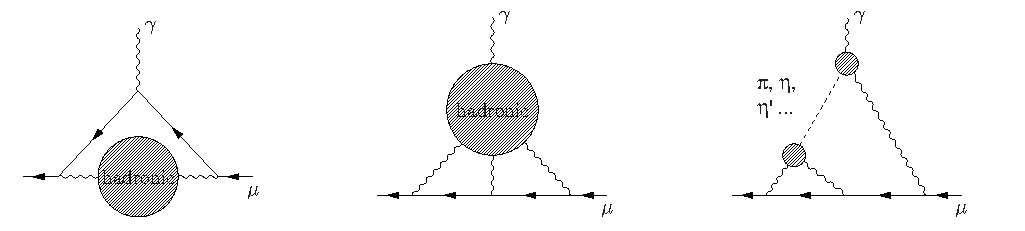
\includegraphics[keepaspectratio,width=1.\textwidth]{figures/intro/hadronicgm2.pdf}
	\caption{Hadronic contributions to $a_\mu$: hadronic vacuum polarization (left diagram), 
		hadronic light-by-light scattering (middle), pion-pole contribution to hadronic light-by-light scattering (right). Full lines with an arrow denote muons, wiggly lines photons, the dashed line a pseudo-scalar meson and shaded blobs a non-pointlike hadronic substructure. The upper blob in the right diagram corresponds to Fig.~\ref{fig:piz.dalitz}, while the lower blob corresponds to the double Dalitz decay. 
	}
	\label{fig:gm2}
\end{figure}

Concerning the SM prediction for $a_\mu$ HLbL is suppressed relative to HVP by one power of the electromagnetic
fine structure constant~\cite{Jegerlehner:2009ry,Bijnens:2007pz}.  
Unfortunately at present it is not possible to straightforwardly 
calculate the contributions shown in Fig.~\ref{fig:gm2} 
from first principles analogously to, e.g., the QED corrections, since
both processes concern low-energy corrections,
i.e.\ non-perturbative physics. Thus the prime candidate for a SM
calculation of hadronic corrections seems to be lattice QCD~\cite{Gattringer:2010zz}. 
However, it is not expected that lattice QCD
results for HPV will reach the required accuracy in the foreseeable future.
For the HLbL only preliminary lattice-QCD calculations have been reported~\cite{Blum:2014oka}.  
In view of the challenges to determine
a four-point function that includes in addition disconnected diagrams
it is not clear yet when a profound lattice calculation with
controlled uncertainties and a reliable error estimate will be
available.

Fortunately there is an alternative way to quantify hadronic corrections. It requires both
theoretical as well as experimental efforts:
Dispersion theory provides a link between particular hadronic cross sections
and $a_\mu$---for a discussion of the HVP in this context see Ref.~\cite{Jegerlehner:2009ry}, while 
for HLbL we refer to Refs.~\cite{Colangelo:2014dfa,Pauk:2014rfa,Colangelo:2014pva,Colangelo:2015ama}.  
In particular for the latter contribution it allows one to calculate from the transition
form factors of the kind $\pi^0$, $\eta$, $\eta'\to \gamma^*\gamma^*$ 
the corresponding piece for the meson pole contribution as displayed in the
right most diagram of Fig.~\ref{fig:gm2}.
The measurements proposed here provide important information towards
the necessary input needed for the evaluation of the HLbL contribution, since
$\eta'\to \gamma^*\gamma$ gives the single off-shell form factor of the $\eta'$
and $\phi\to \eta\gamma$ additionally provides information on the isoscalar
piece of $\eta\to \gamma^*\gamma$ in a different kinematic regime.
Additional information on the  $\eta$ and
$\eta'$ form factors can be found from the dispersive methods outlined in
Refs.~\cite{Adlarson:2011xb,Stollenwerk:2011zz,Hanhart:2013vba,Kubis:2015sga,Xiao:2015uva}.
It  appears to be realistic that this joined effort of theory and experiment
will provide the improvements necessary to push the SM calculation towards
the required accuracy. For the $\etaP$ pole contribution a precision of 15\% on the HLbL correction are feasible.~\cite{Nyffeler}.

\subsection{History}
\indent In the year 1951, Richard Dalitz published a letter~\cite{Dalitz} in which he calculated the rate for the \pizT  decaying into an electron-positron pair (dilepton) and a photon, \pizDal. The calculation assumed that the decay proceeded through a two–photon decay in which one of the photons was virtual and converted into an electron-positron pair.  This kind of reaction is now known as Dalitz decay. The experimental evidence of this decay process was first observed in emulsion plates exposed to the Chicago cyclotron in 1952~\cite{Lord} and a number of experiments performed over the next ten years verified Dalitz’s hypothesis that the \pizDal \ decay resulted from emission of a virtual photon~\cite{Samios,Lindenfeld,Sargent}. A few years later N. Kroll and W. Wada calculated the framework for Dalitz decays within the QED framework~\cite{KrollWada}, and extended the framework to double Dalitz Decays, in which the \pizT decays into two electron-positron pairs via emission of two virtual photons. \\
\indent Throughout the following years, much work was done to extend the framework of Dalitz decays to heavier mesons, such as \etaT, \omT, \etaTP, and \phiT. With numerous experimental data taken, it was shown that the shape of the dilepton mass spectrum deviated from the QED predictions. Such deviations are attributed to the meson not being point-like, as calculated in QED, but instead to the internal structure of the meson. The virtual photon, that decayed into a dilepton pair, has the ability to probe the structure of meson because, like its on-shell counterpart, emission of a  virtual photon is radiation, which decouples from any strong interaction within the meson when the meson transitions into its decay. Therefore, the information of the transition is encoded into the virtual photon, known as the Transition Form Factor (TFF), and can be characterized as $\left| F(q^2)\right|$, where $q^2$ is the square of the invariant mass of the lepton pair. The transition form factor can be determined by comparing QED predictions to the experimentally measured rate. Previous experimental results will be shown in Sec.~\ref{sec:current}.

\subsection{Proposal}
\indent In this proposal we present an experiment to study the $\etaP$ meson which decays via Dalitz decay, \etaPDal. The \etaTP \ is produced via electro-production, $ep \rightarrow ep\etaP$ in Hall B, using the CLAS12 detector. 
The CLAS12 detector will be used to identify and measure the $e^+e^-$ decay products by means of the High Threshold Cherenkov Counter (HTCC), Pre-Calorimeter (PCAL) and Electromagnetic Calorimeter (EC). The combination of HTCC+PCAL+EC can provide a rejection factor for single $e^\pm/\pi^\pm$ of up to $10^5$ for momenta less than 4.9~GeV/c with $\approx$ 100\% efficiency. For dileptons ($e^+e^-$ pairs), this rejection factor will be $\approx 10^{10}$, which enables dilepton studies for branching ratios $\approx 10^{-7}$. Precise determination of momenta and angles of the $e^+e^-$ decay products are the key features available to CLAS12. The momentum and angle of final state photons will be determined in CLAS12 by using the PCAL and EC. Consequently, the photon in the process $\eta^{\prime} \rightarrow e^+e^- \gamma$ will be detected. 
%The superior $e^+e^-$/$\pi^+\pi^-$ discrimination of the CLAS12 detector will give access to measurements for which  $e^+e^-$/$\pi^+\pi^-$ branching ratios of $\gtrsim 10^{10}$ are achievable.
This proposal is organized as follows. In Section~\ref{sec:kinematics}, an explanation of the kinematics of the decay processes will be given as well as kinematics of main competing backgrounds. In Section~\ref{sec:current}, we summarize the current knowledge of Dalitz decays and transition form factors, challenges in dilepton signal quality. Also a brief discussion on past CLAS analysis will be given, along with and how the CLAS12 detector can surpass the current challenges in measuring a TFF, for $\etaP$, of low statistical error. In Section~\ref{sec:measurement} a description of the analysis techniques that have been used and will be used in a CLAS12 measurement. Also in Section~\ref{sec:measurement}, an explanation of the Monte-Carlo simulations that were performed to extract the acceptances will be given as well as a calculation of expected yield and a validity check on the expected yield from previous CLAS analyses. In Section~\ref{sec:beamrequest} we present the beam time request.




\section{Kinematics}\label{sec:kinematics}
The channel proposed to be studied is 
\begin{align}
e(k)+p(p)\to e'(k') + p'(p') +\etaP(\nu) \label{eq:etaP} 
\end{align}
where $k$, $k'$, $p$, $p'$ are the four–momenta of the incident lepton, outgoing lepton,target proton and scattered proton respectively. The virtual photon in the production is defined as $q=k-k'$ with energy $v = \frac{pq}{m_p} = E - E'$. The quantity $\etaP(\nu)$ is the electro-produced meson. Production mechanisms of similar mesons have been already proposed in previous proposals~\cite{clas.proposal.eta,clas.proposal.phi} and are scheduled to run in conjunction with RunGroupA, the same run group requested for in this proposal.
The main decays studied for this proposal are:
\begin{align}
\etaP \rightarrow \gamma \gamma \to e^+e^- \gamma \label{eq:etaPconv} \\
\etaP \rightarrow \gamma \gamma^\star \to \gamma e^+e^- \label{eq:etaPDal} 
\end{align}
i.e. when a pseudoscalar meson, $P_p$($\eta'$), decays via two photons (Eq.~\ref{eq:etaPconv}) and one photon converts into an \epemT \ pair due to E.M. processes through matter, this is conventionally known as external conversions. This decay channel will he the main background contribution and in further discussed in Sec~\ref{sec:intro.conversion}. The Dalitz decay, or internal conversion, is when the $P_p$($\eta'$) decays via a real photon and a virtual photon (Eq.~\ref{eq:etaPDal}), which decays into an \epemT \ pair.
Figure~\ref{fig:piz.alldecay} illustrates the Feynman diagrams for the pseudoscalar ``two photon decay'' and  ``Dalitz decay''.
 %Table~\ref{tab:pi0}. Figure~\ref{fig:piz.alldecay} illustrates the Feynman diagrams for the ``Two photon decay'' and the ``Dalitz decay''.
 \begin{figure}[h!]\begin{center}
 		\subfloat[Feynman Diagram of $\etaP$ Two Photon Decay][]{ %Feynman diagram of $\etaP$ two photon decay
 			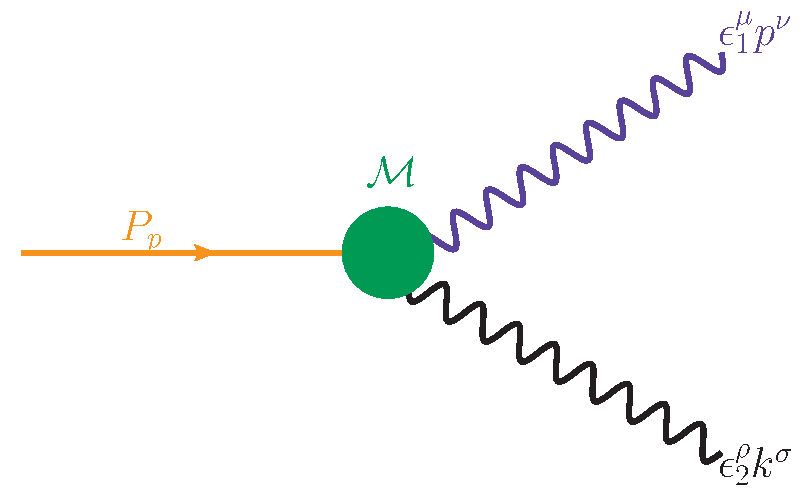
\includegraphics[width=0.4\columnwidth,height=0.75\qfigheight]{\grpath/decays/psudoscalar_gammagamma.pdf}\label{fig:piz.gamgam}
 		}
 		\quad
 		\subfloat[Feynman Diagram of $\etaP$ Dalitz Decay][]{ %Feynman diagram of $\etaP$ Dalitz decay
 			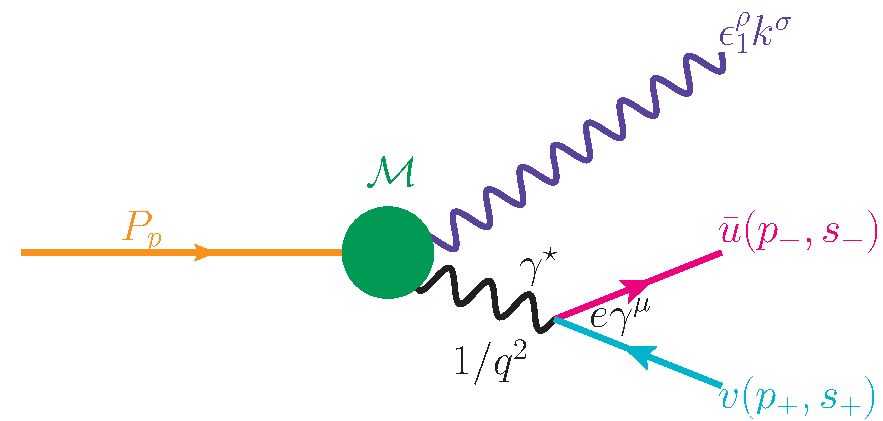
\includegraphics[width=0.45\columnwidth,height=0.75\qfigheight]{\grpath/decays/psudoscalar_dalitz.pdf}\label{fig:piz.dalitz}
 		}
 		\caption[Feynman diagram of $P_p$($\etaP$) two photon decay and Dalitz decay]{\label{fig:piz.alldecay}Feynman diagram of $P_p$($\etaP$) two photon decay~\subref{fig:piz.gamgam}, $\epsilon_1$ and $\epsilon_2$ are the polarizations, $p$ and $k$ are 4-momenta of the photons.  Feynman diagram of $P_p$($\etaP$) Dalitz decay~\subref{fig:piz.dalitz}, the variable $s_\pm$ are the spin helicities of the outgoing leptons $l^\pm$ with 4-momenta $p_{\pm}$ and $\epsilon$ is the polarization of the outgoing photon with 4-momenta $k$. In both diagrams $\mathcal{M}$ is the form factor.}
\end{center}\end{figure}
 A full derivation of the external conversion and Dalitz decay are given in the Appendix~\ref{sec:app.kinematics}.
 \FloatBarrier
  \subsection{The Dalitz Decay}
  The Dalitz decay of mesons is dependent on the spin of the meson. For pseudoscalar meson the decay rate is derived in~\ref{sec:dalitzdecay} and is expressed as:
  \begin{align}\label{eq:eegff.finalkroll_II}
  \frac{d\Gamma_{\epem \gamma}}{\Gamma_{\gamma\gamma} dq^2} = \frac{2 \alpha}{3 \pi} \frac{1}{q^2} \left( 1- \frac{q^2}{m_p^2}\right)^3 \left( 1+ \frac{2m_l^2}{q^2}\right) \left( 1- \frac{4m_l^2}{q^2}\right)^{\frac{1}{2}} 
  \end{align}
  which is the Kroll-Wada equation founded in~\cite{KrollWada,landsberg}.
   An example of QED expectation for \etaTP  \ is shown in Fig.~\ref{fig:dalitz_compare}.
  \subsection{Form Factor}
   It has been experimentally observed that the shape of the dilepton mass spectrum deviates significantly from the QED predictions, displaying a rise at larger dilepton mass. Therefore, the form factor ${M}_P(p^2,k^2=0)$ or ${M}_P(p_{1}^2,p_{2}^2)$  can be written as follows:
  \begin{align}
  {M}_P \to {M}_P' \times \left|F(q^2)\right| \ ,
  \end{align}
  where $M_P'$ is the decay constant of two photons or $\eta$ photon (as mentioned in Sec.~\ref{sec:piz.gg}), while $\left|F(q^2)\right|$ is called the transition form factor, which defines the electromagnetic space structure of the meson. According to that, the $\etaP \to e^+e^- \gamma$ the decay rate modifies as;
  \begin{align}\label{eq:eegff.final}
  \frac{d\Gamma_{\epem \gamma}}{\Gamma_{\gamma\gamma} dq^2} = \frac{2 \alpha}{3 \pi} \frac{1}{q^2} \left( 1- \frac{q^2}{m_p^2}\right)^3 \left( 1+ \frac{2m_l^2}{q^2}\right) \left( 1- \frac{4m_l^2}{q^2}\right)^{\frac{1}{2}} \left|F(q^2)\right|^2 \ ,
  \end{align}
  First observations were described with standard vector meson dominance (VMD) where the virtual photon can stem from a intermediate vector mesons. 
  The value of $\left|F(q^2)\right|$ can be directly measured by comparing QED predictions to the measured rate~\cite{landsberg}. 
  \begin{align}
  \frac{d\Gamma(A\to B+l^+l^-)}{dq^2 \Gamma(A\to B\gamma)} = \left[\frac{d\Gamma}{dq^2}\right]_{\text{QED}} \cdot \left | F(q^2) \right |^2 
  \end{align}
  or by performing a line shape analysis on the $l^{+}l^{-}$ invariant mass using assumptions on the structure of $\left|F(q^2)\right|$. One such assumption for $\left|F(q^2)\right|$ is the dipole approximation from the VMD model, which can be parametrized as:
  \begin{align}
  F(q^2) = \frac{1}{1-q^2/\Lambda^2} 
  \end{align}
   where the parameter $\Lambda$ corresponds to the mass for the effective contributing vector meson.
%  , in which 
%  \begin{align}
%  F(q^{2}) = \frac{\Lambda^2(\Lambda^2 + \gamma^2)}{(\Lambda^{2} - q^2) + \Lambda^2\gamma^2 } \nonumber
%  \end{align}
%  where the parameters $\Lambda$ and $\gamma$ correspond to the mass and width of the Breit-Wigner shape for the effective contributing vector meson. A first approximation is that $\Lambda \approx M_{\rho} \approx 0.7$~GeV and $\gamma \approx \Gamma_{\rho}  \approx 0.12$~GeV. A comparison showing the QED spectra and the deviation from QED using the VMD parameterization is shown in Fig.~\ref{fig:dalitz_compare} for \etaTP  \ and $\phi$.

 The slope of the transition form factor, $b$, is defined as:
\begin{align}
b \equiv \frac{dF}{dq^2}|_{q^2=0} \label{eq:tffslope}.
\end{align}
and characterizes the intrinsic spatial charge radius for the $\etaP$ meson, and the $\phi \to \eta$ transition for the $\phi$ meson.
 \begin{figure}[h!]\begin{center}
 		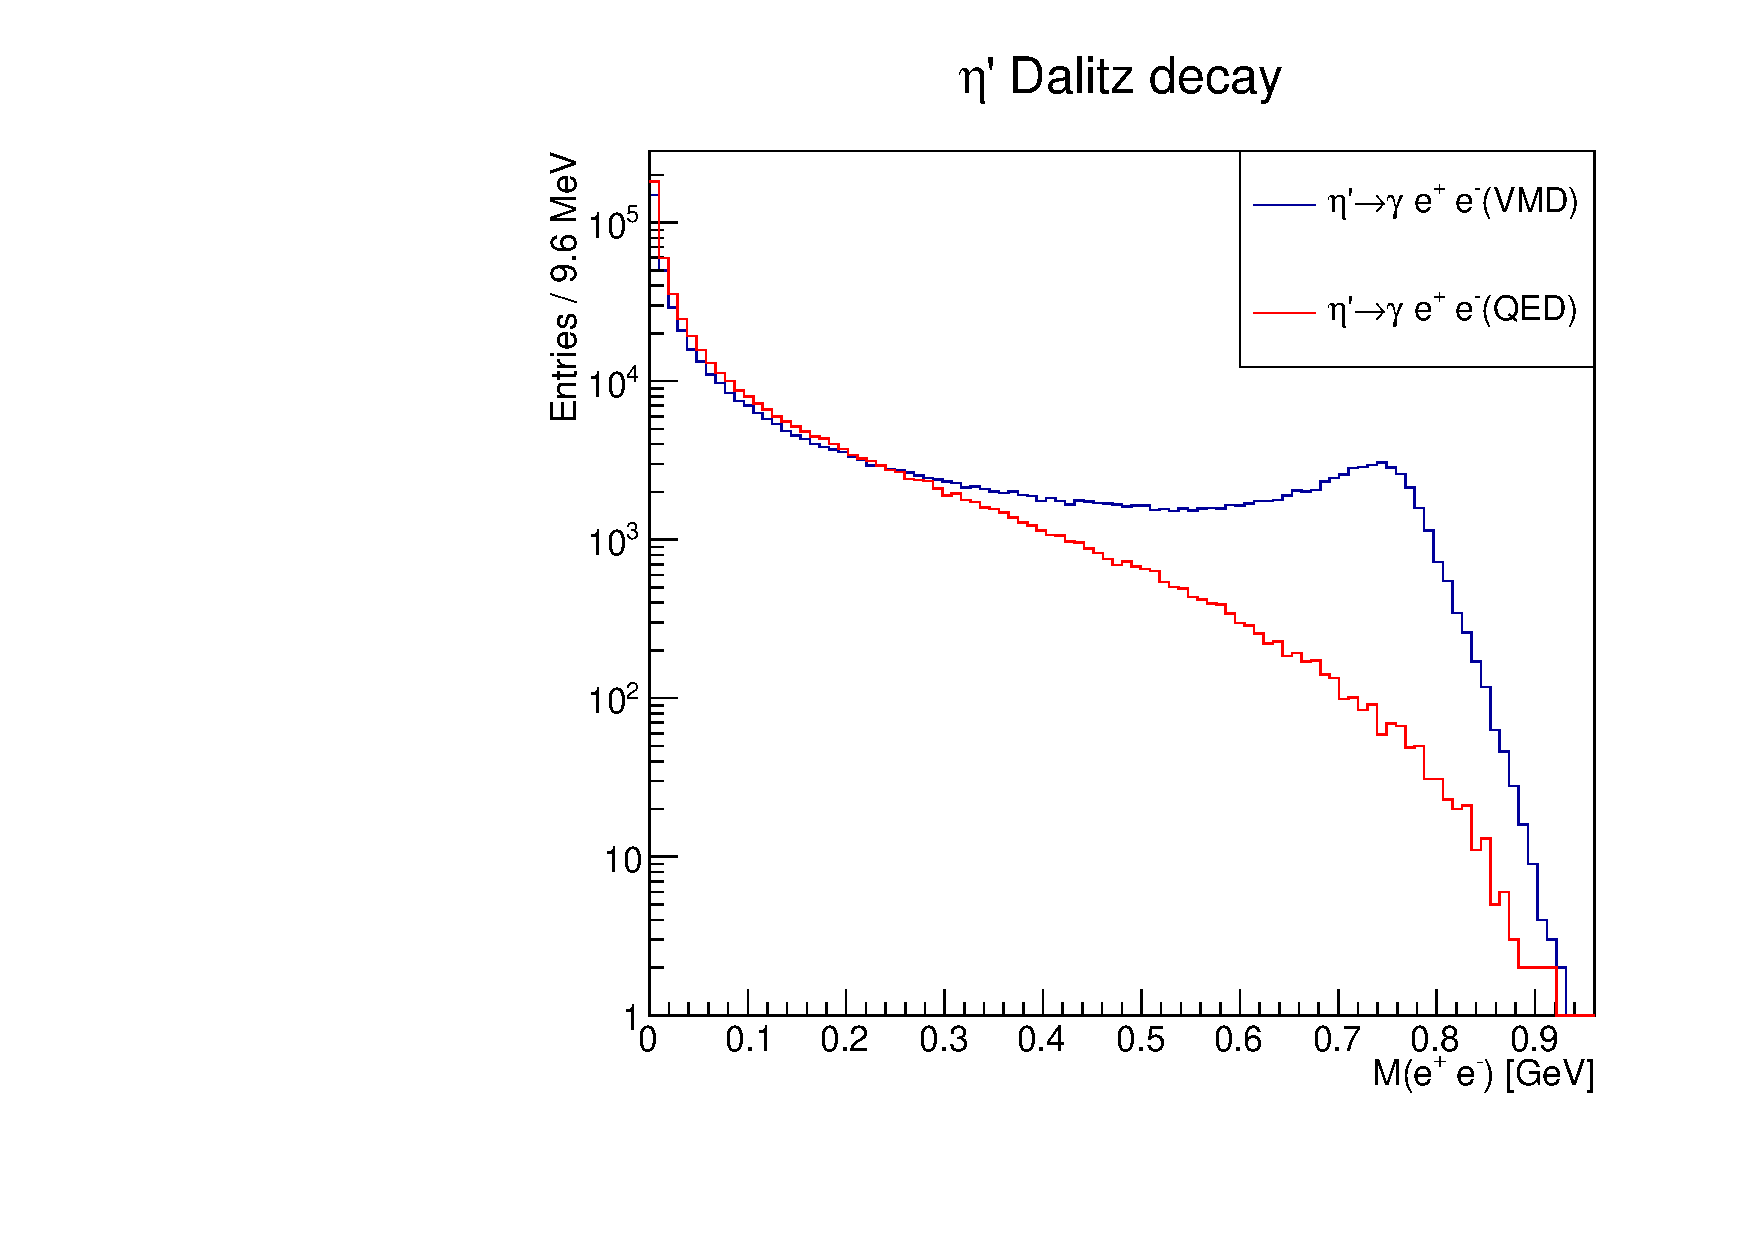
\includegraphics[width=0.8\columnwidth,height=1.0\qfigheight]{\grpath/decays/etaP_Dalitz_QED_FF_comparePlot.pdf}\label{fig:etap_dalitz_conpare}
 		\caption[Dalitz  for \etaTP \ and $\phi$]{\label{fig:dalitz_compare}Example of Dalitz spectra for \etaTP \ using only QED(red) and the deviation from QED using the VMD parameterization(blue) with 500K Dalitz events generated~\subref{fig:etap_dalitz_w_conversion}. }
 	\end{center}\end{figure}



% \begin{figure}[h!]\begin{center}
% 		\subfloat[$\etaP$ Dalitz spectra][]{ %Feynman diagram of $\etaP$ two photon decay
% 			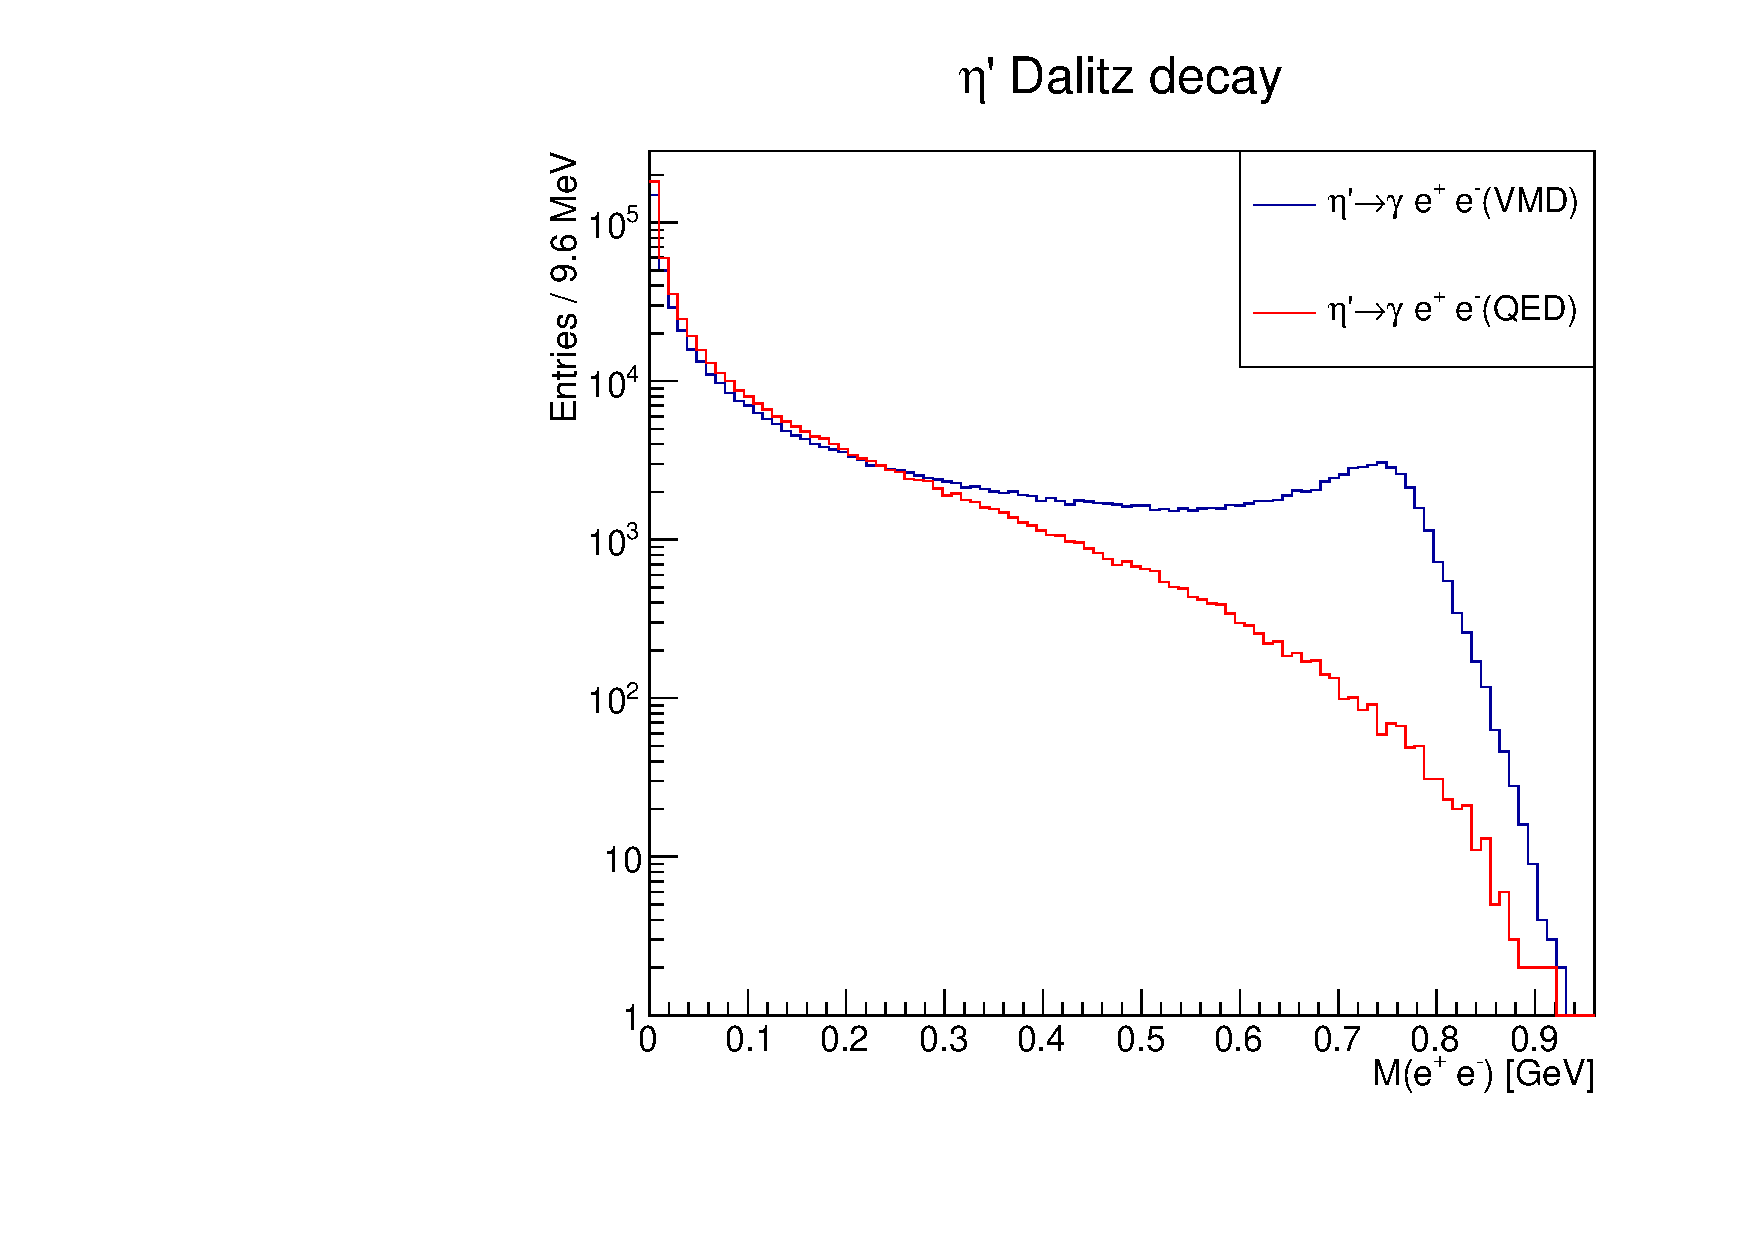
\includegraphics[width=0.8\columnwidth,height=1.0\qfigheight]{\grpath/decays/etaP_Dalitz_QED_FF_comparePlot.pdf}\label{fig:etap_dalitz_conpare}
% 		}
% 		%\quad 
% 		\\
% 		\subfloat[$\phi$ Dalitz  spectra][]{ %Feynman diagram of $\etaP$ Dalitz decay
% 			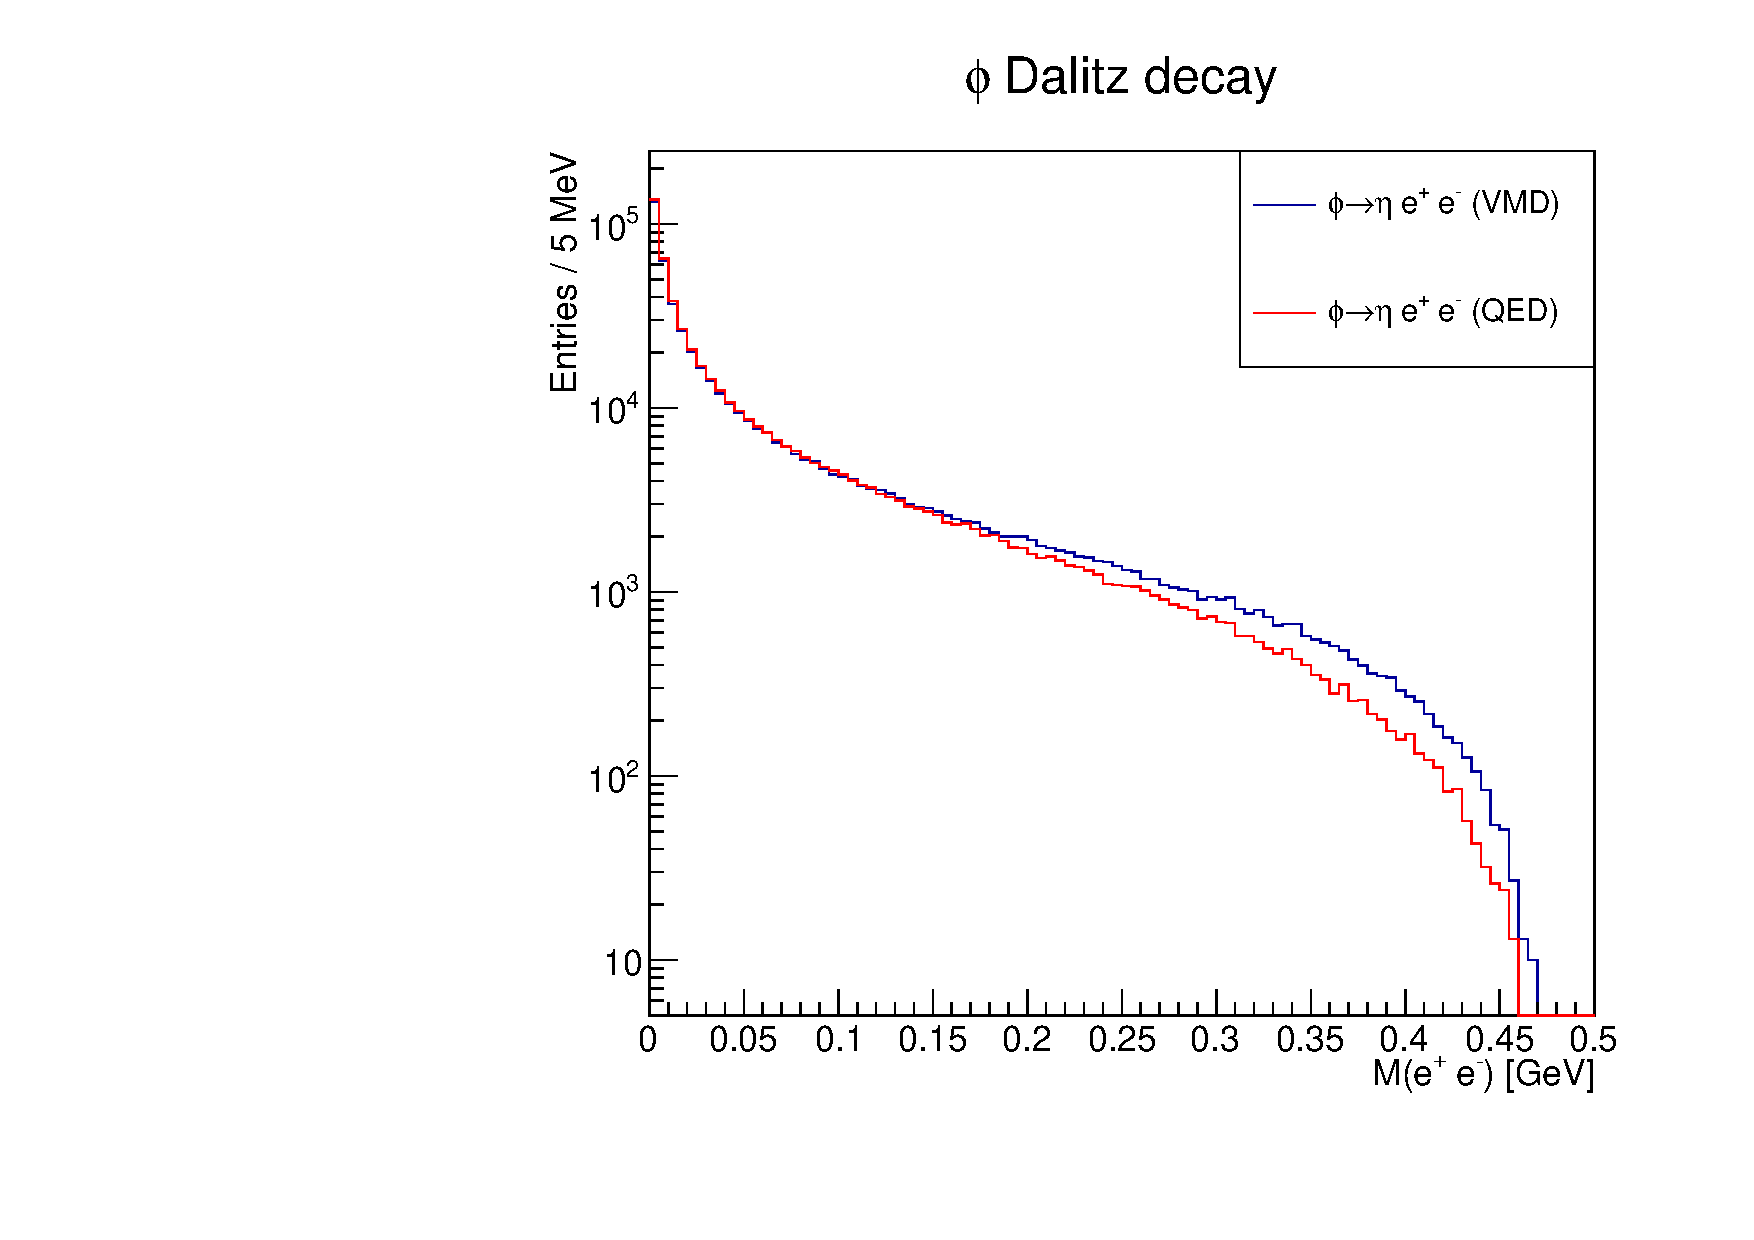
\includegraphics[width=0.8\columnwidth,height=1.0\qfigheight]{\grpath/decays/phi_Dalitz_QED_FF_comparePlot.pdf}\label{fig:phi_dalitz_compare}
% 		}
% 		\caption[Dalitz  for \etaTP \ and $\phi$]{\label{fig:dalitz_compare}Example of Dalitz spectra for \etaTP \ using only QED(red) and the deviation from QED using the VMD parameterization(blue) with 500K Dalitz events generated~\subref{fig:etap_dalitz_w_conversion}.  Example of Dalitz  spectra for $\phi$ using only QED(red) and the deviation from QED using the VMD parameterization(blue)  with 500K Dalitz events generated~\subref{fig:phi_dalitz_w_conversion}. }
% 	\end{center}\end{figure}
\FloatBarrier 	 
\subsection{Photon Conversion to \epemT Pairs}\label{sec:intro.conversion}
When a photon travels through matter at energies greater than 100~MeV, it can convert into an electron-positron pair. The process of pair production, $\gamma Z \rightarrow Ze^{+}e^{-}$, occurs when a photon with $E_0 > 2 m_e c^2$ converts into an electron and a positron. The cross section for this process can be written as;
\begin{equation}\label{pair_crosssection}
\sigma_{\gamma\rightarrow e^+e^-} =  \frac{A}{N_{A} \rho \lambda_\gamma}  \ ,\ \lambda_\gamma = \frac{9}{7}X_0
\end{equation}
where $\lambda$ is the interaction length, or mean free path, $\rho$ is the density of the material, $N_A$ is Avogadro's number and $A$ is the atomic mass of the material. The probability of pair production to occur is solely based on $X_{0}$, the radiation length of the medium and this probability can be expressed as;
\begin{equation}
\frac{dP}{dx} = \frac{1}{\lambda_\gamma}\exp(\frac{-x}{\lambda_\gamma}) \ .
\end{equation}
%
%
Using the ratio, $\frac{\Gamma_{\etaP \to e^+e^- \gamma}}{\Gamma_{\etaP \to \gamma \gamma}} = 2.13\cdot 10^{-2}$, that has been preliminary measured by CLAS, which is consistent with~\cite{BESIII}, the probability of pair production when a photon, from the $\etaP \to \gamma \gamma$ decay, traveling though 5~cm of liquid hydrogen, $\ell$H$_2$, is shown in Fig.~\ref{fig:conversion} as well as the number of $\etaP \to \gamma \gamma \rightarrow e^+e^- \gamma$ / $100 \etaP \rightarrow e^+e^- \gamma$. 
\begin{figure}[h!]\begin{center}
	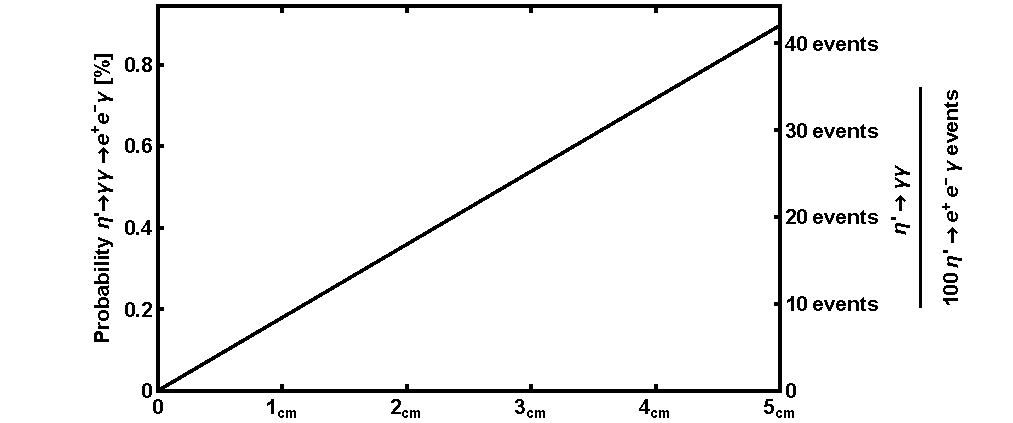
\includegraphics[width=\figwidth,height=\qfigheight]{\grpath/decays/cmplot.pdf}
	\caption[Probability of pair production, $\gamma \to$\epemT, as a function of distance in liquid hydrogen]{\label{fig:conversion}{(Left axis)Probability of pair production, $\gamma \to$\epemT; (Right axis) number of $\etaP \to \gamma \gamma \rightarrow e^+e^- \gamma$ / $100 \etaP \rightarrow e^+e^- \gamma$ as a function of distance in liquid hydrogen.}}
\end{center}\end{figure}
	Since CLAS12 has a vertex resolution of $\approx$1~mm the probability of pair production traveling through 10~mm is shown in Fig.~\ref{fig:conversionmm}. Therefore, a 1~mm cut on the primary vertex will yield a contamination of $\approx$ one externally converted \epemT from $\etaP \to \gamma \gamma \rightarrow e^+e^- \gamma$ per Dalitz decays $100 \etaP \rightarrow e^+e^- \gamma$
\begin{figure}[h!]\begin{center}
	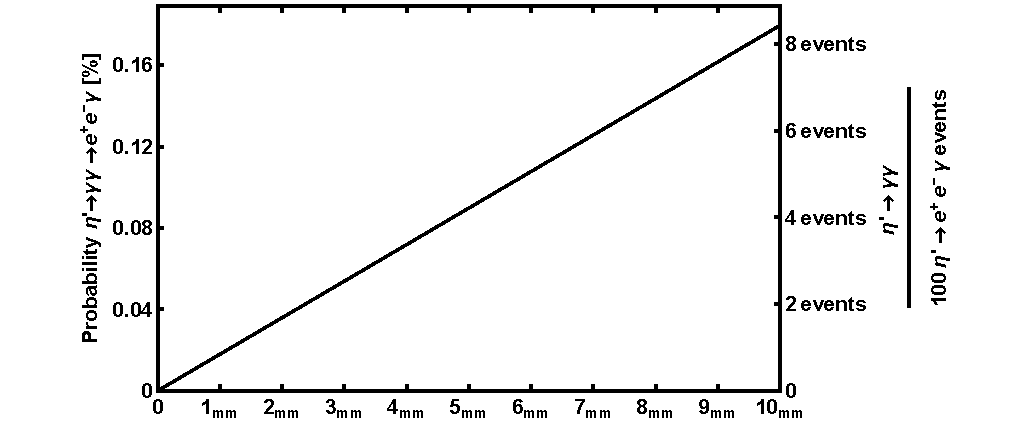
\includegraphics[width=\figwidth,height=\qfigheight]{\grpath/decays/mmplot.pdf}
	\caption[Probability of pair production, $\gamma \to$\epemT, as a function of distance in liquid hydrogen]{\label{fig:conversionmm}{(Left axis)Probability of pair production, $\gamma \to$\epemT; (Right axis) number of $\etaP \to \gamma \gamma \rightarrow e^+e^- \gamma$ / $100 \etaP \rightarrow e^+e^- \gamma$ as a function of distance in liquid hydrogen.}}
\end{center}\end{figure}
This type of subprocess mimics the Dalitz decay  $\etaP \to e^+e^- \gamma$, described in Sec.~\ref{sec:dalitzdecay}. Since there are two photons with equal probability of conversion for $\etaP \to \gamma \gamma$, the total probabilities shown is for when either photon externally converts.
From multiple scattering effects the \epemT \ from a converted photon will obtain a mass distribution. Simulations of photons from \etaTP \ and $\phi$ radiative decays traversing through 1~mm of $\ell H_2$  show that the \epemT can obtain a maximum mass of $\sim 0.14$~GeV.		
\begin{figure}[h!]\begin{center}
		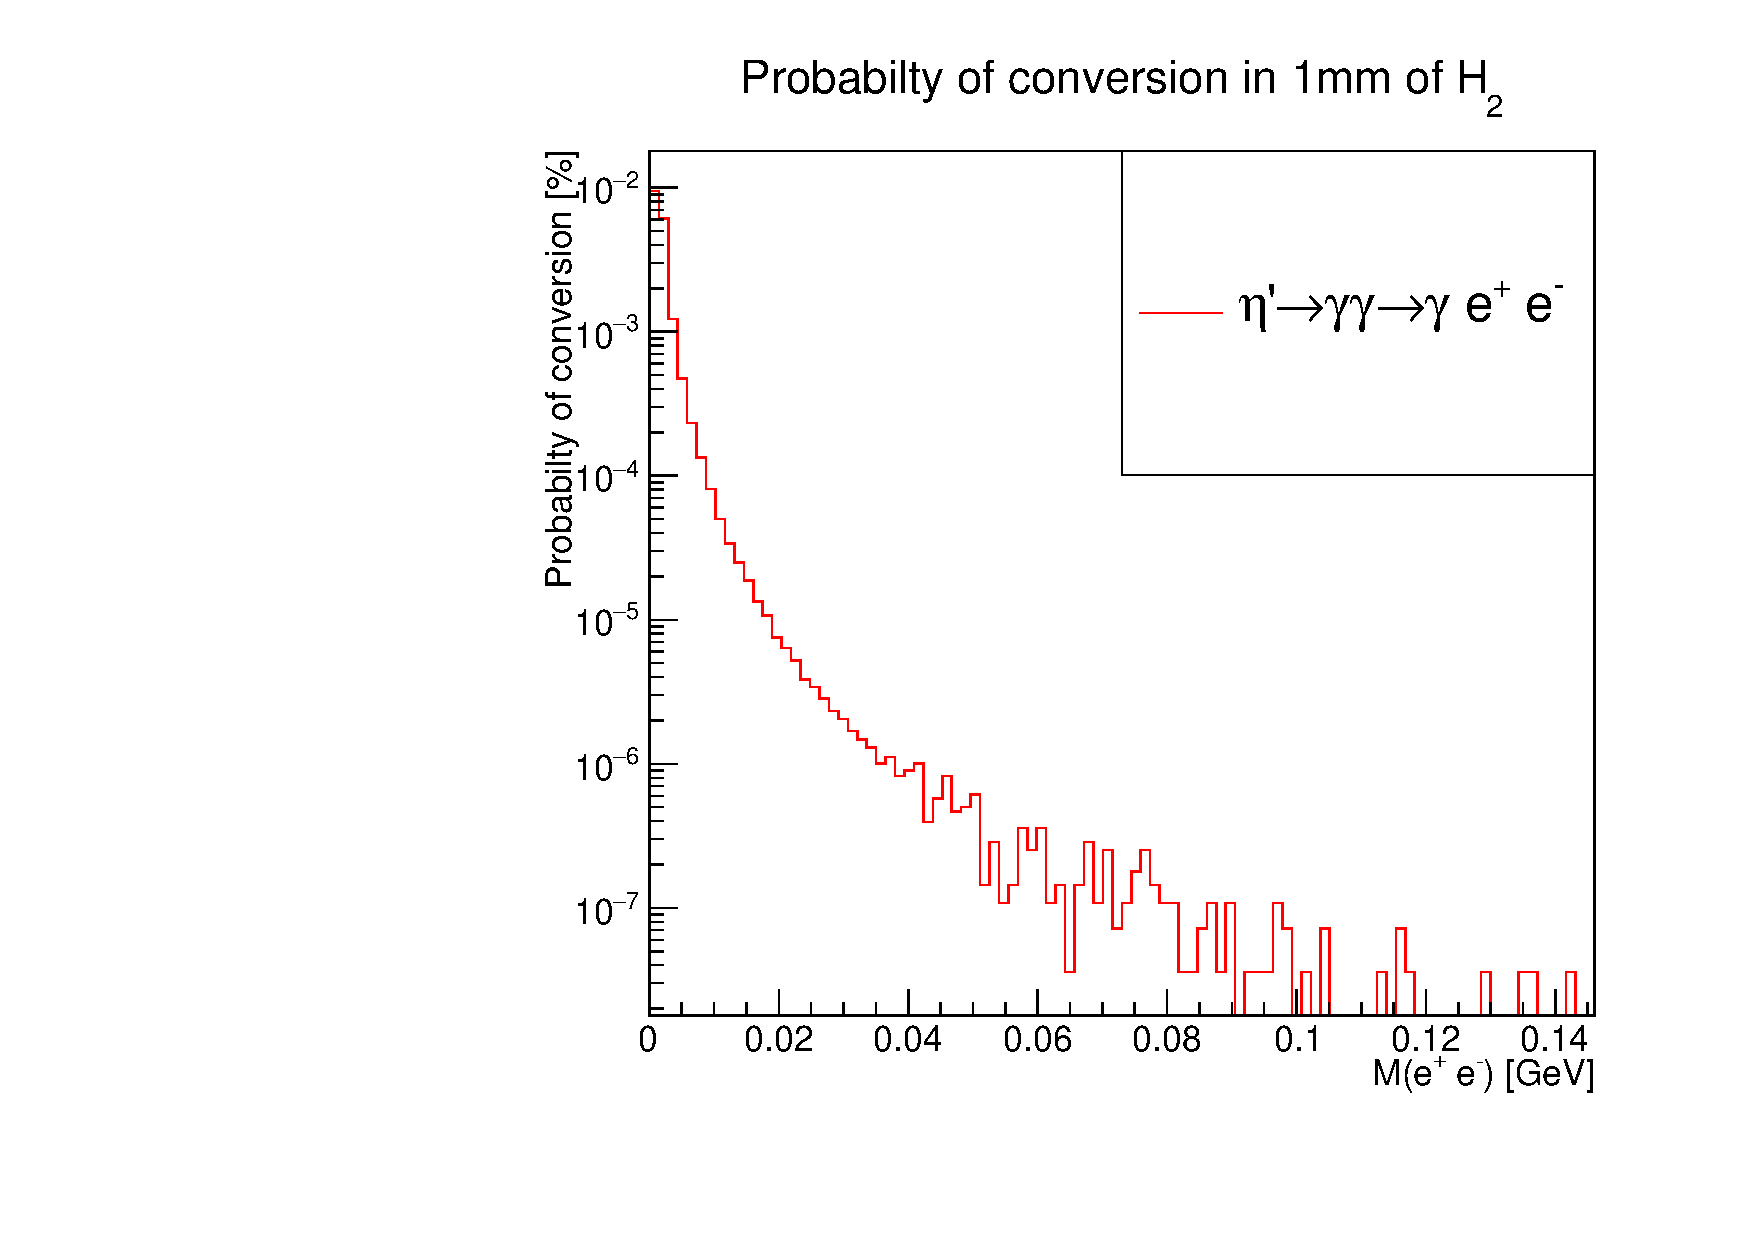
\includegraphics[width=\figwidth,height=1.2\qfigheight]{\grpath/decays/etaP_total_conversionPlot.pdf}
		\caption[Probability of pair production, $\gamma \to$\epemT, as a function of $M(\epem)$]{\label{fig:conversion_inM}{Probability of pair production in 1~mm of  $\ell H_2$ for $\etaP \to \gamma \gamma $ vs. $M(\epem)$.}}
\end{center}\end{figure}
 \subsection{Summary}
 The $\gamma \gamma$ decay and the $\gamma^\star \gamma$ decay have different branching ratios. This difference is attributed to the factor of $\alpha$ along with a $q^2$ dependence calculated in the Dalitz decay. However, due to the probability of a photon converting into an electron-positron pair in $\ell$H$_2$, the total amount of \epemT pairs produced via photon conversion can contaminate the measurement of the form factor. The CLAS detector will have vertex resolution of $\sim$1~mm, therefore the amount of contamination of externally converted pairs will be minimized by the vertex position of the \epemT pair. An example of the total contamination, in the Dalitz spectrum, from external conversion within 1~mm of the primary vertex can be seen in Fig.~\ref{fig:dalitz_w_conversion}.
 \begin{figure}[h!]\begin{center}
 			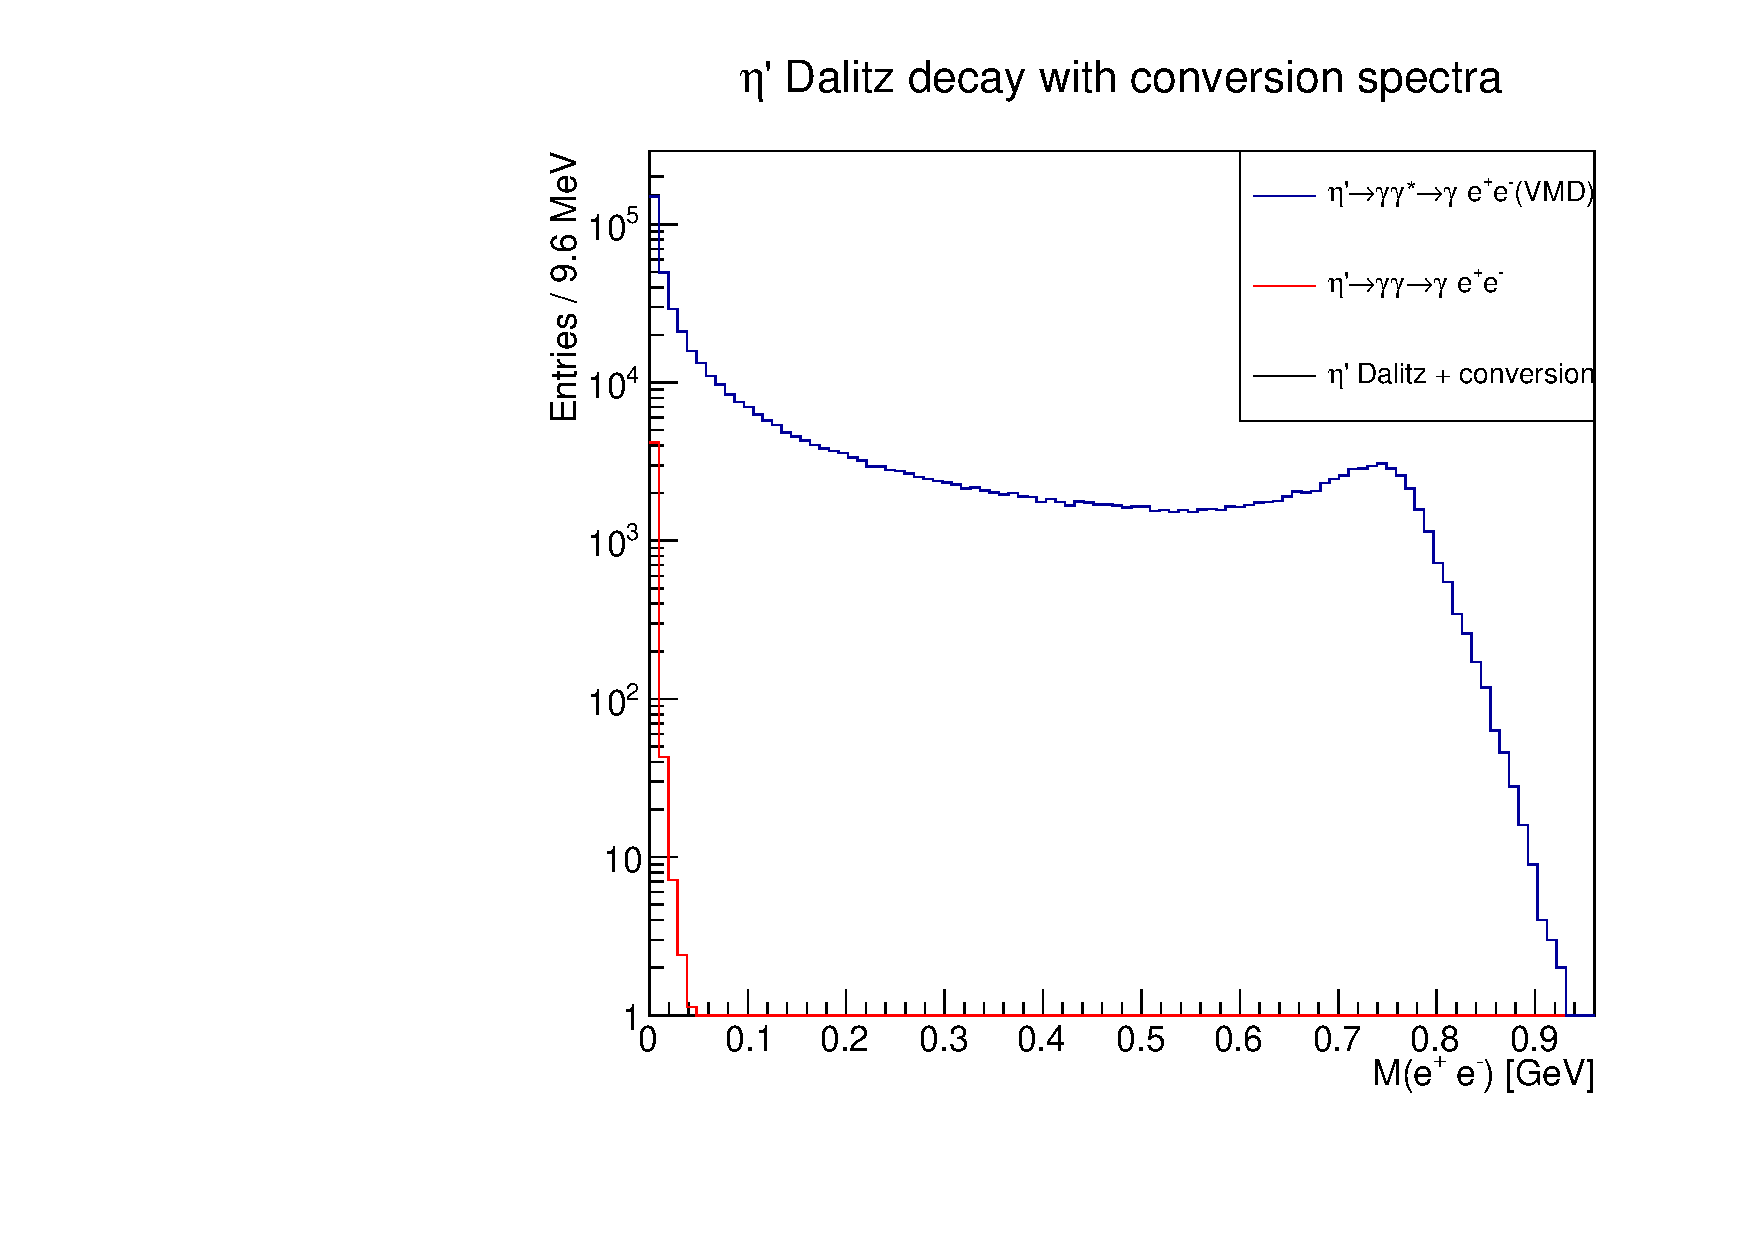
\includegraphics[width=0.8\columnwidth,height=1.0\qfigheight]{\grpath/decays/etaP_Dalitz_decay_with_conversion_spectra.pdf}
\caption[Dalitz and conversion spectra for \etaTP \ and $\phi$]{\label{fig:dalitz_w_conversion}Example of Dalitz and conversion spectra for \etaTP \ with 500K Dalitz events generated and $\sim 2.35 \cdot 10^7$ $\etaP \to \gamma \gamma$ generated.}
\end{center}\end{figure}
\FloatBarrier
  
  
  
\section{Current Experimental Measurements}\label{sec:current}
Several experimental groups are currently investigating transition form factors in the time-like regime, including, but not limited to;
\begin{itemize}
	\item TRIUMF $\pi^0 \to \epem \gamma$~\cite{FARZ} 
	\item A2 Collaboration $\eta \to \epem \gamma$~\cite{Berg,A2} 
	\item Multiple Groups $\omega\to\pi^0 \mu^+\mu^-$ ~\cite{Dzhelyadin:1980tj,Arnaldi:2009aa,Uras:2011zz}
	\item CLEO Collaboration $\eta'\to e^+e^-\gamma $~\cite{CLEO}
	\item Lepton-G $\eta'\to \mu^+\mu^-\gamma $~\cite{DZH}
	\item BESIII Collaboration $\eta'\to e^+e^-\gamma $~\cite{Ablikim:2015wnx}
	\item KLOE Collaboration $\phiDalT$~\cite{Babusci:2014ldz} .
\end{itemize}
The branching ratio of \etaPDal \ remained an upper limit, Fig.~\ref{fig:past}, until the BESIII collaboration finally measured it using 1.31 billion $J/\psi \to \gamma \etaP \to \gamma \gamma \epem$. From the BESIII data sample, Fig.~\ref{fig:past}, only 894 \etaPDal \ events were recorded which lead to a determination of the branching ratio $\Gamma_{\eta^{\prime} \rightarrow e^+e^- \gamma}  = 4.69 \pm 0.2 (\mathrm{stat.})\cdot 10^{-4}$ and a slope parameter, Eq.~\ref{eq:tffslope}, $b = 1.60\pm0.17(\mathrm{stat.})$ which is consistent with the measurement from Lepton-G ($1.7 \pm 0.4 (\mathrm{stat.})$). The slope parameter measured by BESIII and Lepton-G, which is the essential measurement needed for the HLbl contribution, is not sufficient to distinguish between different theoretical approaches listed in Tab.~\ref{tab:theory}. Some of the obstacles for not measuring the \etaPDal \ was the low branching ratio, pion contamination and low electron PID efficiency. These obstacles will be mitigated with CLAS12 by the high luminosity and excellent dilepton identification.

%The experiential results of the $\pi^0$ and $\omega$ present a puzzle because for the $\pi^0$ the measurement in the time-like region does not have agreement between several experiemtn
%
%The experimental results on the conversion decay of the $\omega$ meson, $\omega\to\pi^0 \mu^+\mu^-$  present a puzzle ~\cite{Dzhelyadin:1980tj,Arnaldi:2009aa,Uras:2011zz}. 
%The measurements suggest a dramatic increase of the transition form factor for large momentum transfers that is not consistent with VMD models nor explicable with modern theoretical advances. 
%These experimental results are in contradiction to measurements in the space-like regime~\cite{Achasov:2013btb}. 
%The situation makes it important to investigate the conversion decays of vector mesons. 
%
%{\it ... mention A2 measurement ? ...}
%
%The conversion decays of the  $\omega$ meson are currently being studied within the LMD group using data from the CLAS g12 experiment. 
%We plan to approach the conversion decays of the $\phi$ meson by analyzing the decay $\phi\to\eta\gamma^\star$ based on the proposed experiment. 
%The decay $\phi \to \pi^0\gamma^\star$ would enable access to higher dilepton masses and more precise mapping of transition form factors in this kinematic regime. However, the decay is OZI suppressed and statistically significant results may be obtained after a luminosity upgrade of the experiment facility.
%Current measurements by the KLOE collaboration for $\phi\to\eta e^+e^-$~\cite{Babusci:2014ldz} and $\phi\to\pi^0 e^+e^-$~\cite{Anastasi:2016bfh} have improved the values for the respective branching ratios by the SND and CMD-2 collaborations ~\cite{Achasov:2000ne,Akhmetshin:2000bw,Achasov:2002hs,Akhmetshin:2000wi}. The $\phi\to\eta e^+e^-$ measurement by KLOE is based on ~31000 events and deduces a slope parameter of $ \text{KLOE} \ b_{\phi\eta}=1.28\pm 0.10^{+0.09}_{-0.08} $.
%
%{\it ... figure of KLOE phi-eta TFF here? ...}
\begin{figure}[h!]\begin{center}
		\subfloat[$\phi$ Dalitz and conversion spectra from g12][]{ %Feynman diagram of $\etaP$ Dalitz decay
			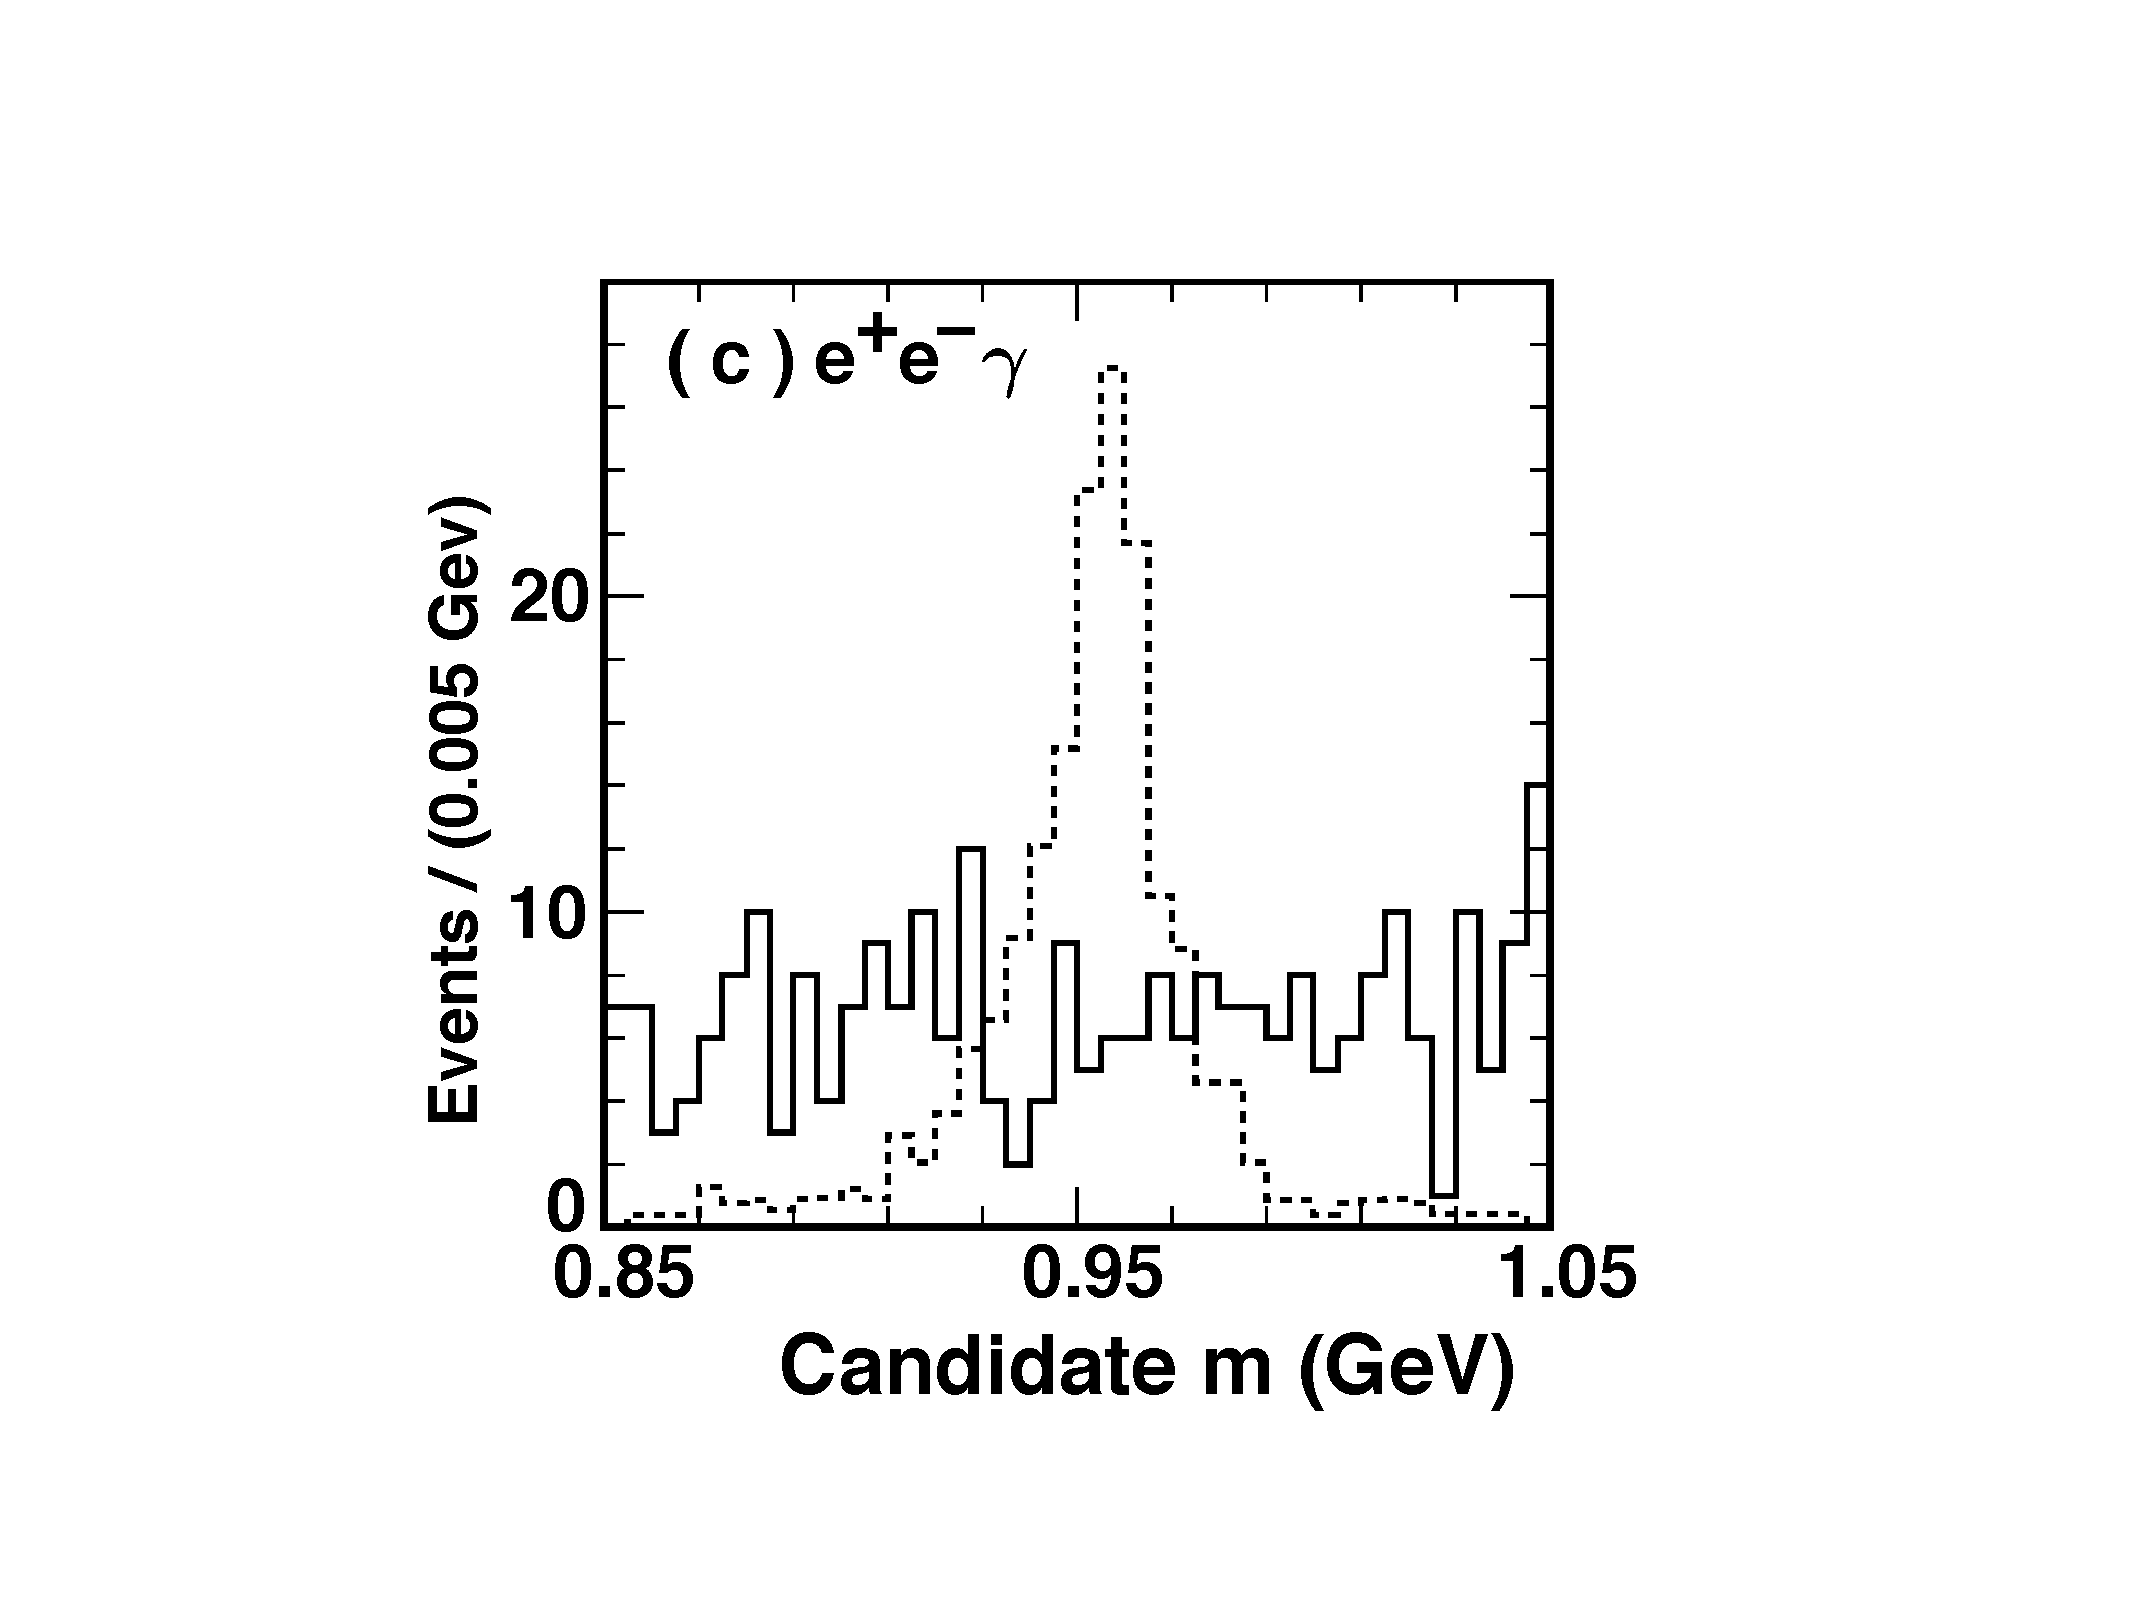
\includegraphics[width=1.0\columnwidth,height=1.0\qfigheight]{\grpath/current_status/CLEO_keynote.pdf}\label{fig:CLEO}
		}
		\\
		\subfloat[$\etaP$ Dalitz and conversion spectra from BESIII][]{ %Feynman diagram of $\etaP$ two photon decay
			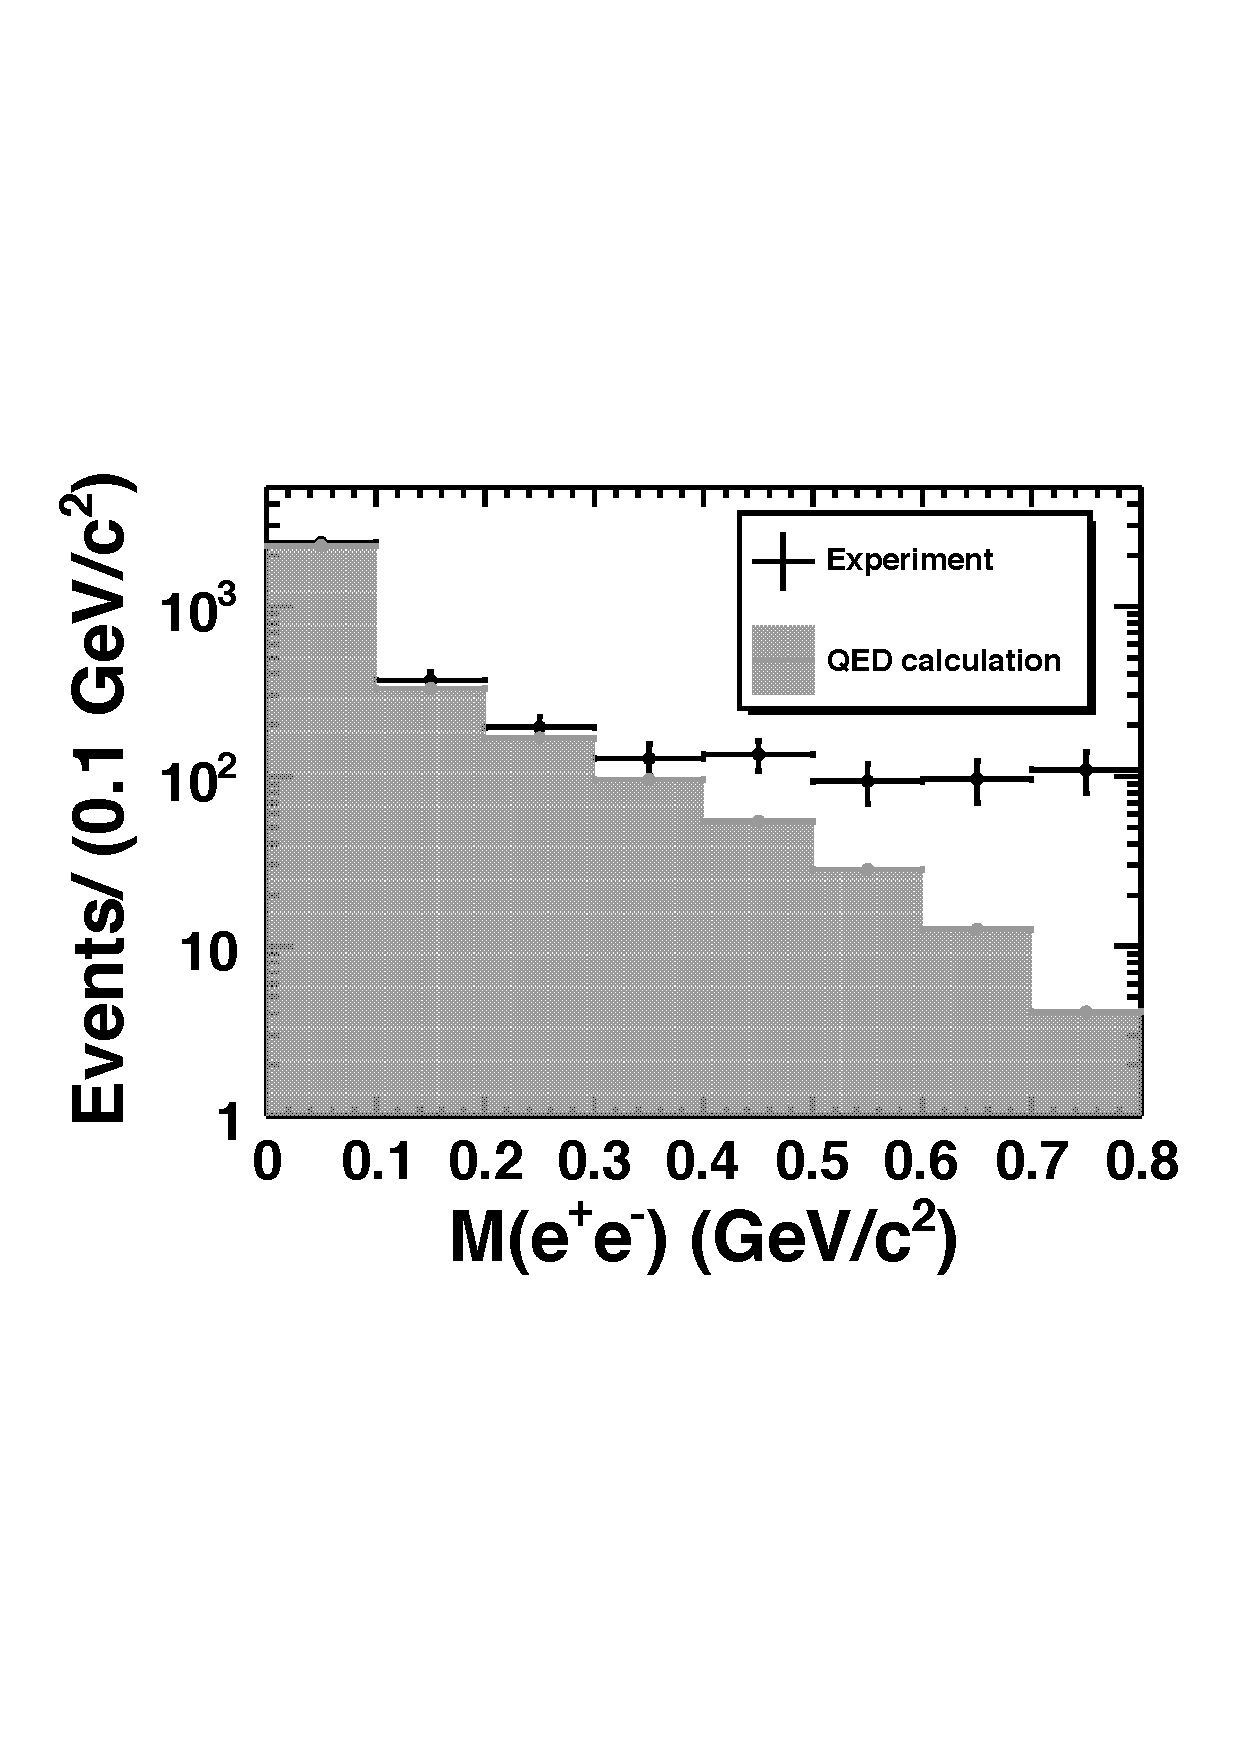
\includegraphics[width=0.8\columnwidth,height=1.8\qfigheight]{\grpath/current_status/BESIII_EtaP.pdf}\label{fig:BESIII}
		}
		\caption[Counts rates for \etaTP from previous experiements]{\label{fig:past} ~\subref{fig:CLEO} Missing mass off of the proton for \etaPDal \ from the CLEO collaboration~\cite{CLEO}, solid line(data), dashed(MC expectation).~\subref{fig:BESIII}Counts of $M(\epem)$ from the first published observation of the \etaPDal \  by BESIII~\cite{BESIII}. }
\end{center}\end{figure}
	\FloatBarrier 	
	\subsection{Previous CLAS analyses}
	The LMD (Light Meson Decay) group of CLAS was established to investigate the decay properties of light mesons. Two experiments in CLAS are currently being analyzed in the LMD group. The g12 experiment, performed with CLAS, is one experiment chosen due to its ability to identify leptons with the use of the Cherenkov detectors (CC).
	% performed with the g12 experiment
	The g12 experiment produced a data set of photon-induced reactions. Fortunately, the Cherenkov Counters were filled with perflourbutane ($C_4F_{10}$) and a trigger consisting of a coincidence between the (ST$\cdot$TOF)(CC$\cdot$EC), allowing the study of dilepton reactions throughout the entire beam energy range $1.15 \ \mathrm{GeV}<E_\gamma <5.45 \ \mathrm{GeV}$. The g12 experiment ran for 44 days however, the trigger that allowed for \epemT identification was established for $\sim$29 days of beam-time. Using approved dilepton identification~\cite{g12note}, preliminary analyses of g12 involving dileptons include the decays:
	\begin{itemize}
		\item $\Delta \to p \epem$ (Transition form factor)
		\item $\eta \to \epem \gamma$ (Transition form factor)
	\end{itemize}
	while advanced analyses involving dileptons include:
	\begin{itemize}
		\item $\piz \to \epem \gamma$ (Differential Cross-Section)
		\item $\omega / \rho \to \epem$ (Interference of $\omega/\rho$ )
		\item $\omega \to \epem \piz$ (Transition form factor)
		\item $\etaP \to \epem \gamma$ (Transition form factor / branching ratio)
	\end{itemize}
	The g12 \etaPDal \ analysis provided CLAS its first look at the possibility of measuring the branching ratio and transition form factor. 
	\subsubsection{G12 Lepton and Neutral Trigger Setup}\label{sec.data.trig.lepton}
In g12, since the CC was filled with gas, it was possible to include the CC as a component of the trigger. 
There were three trigger ``bits'' used for lepton identification in g12 as listed in Tab.~\ref{tab:data.trig.conf.2}. Each ``bit'' used a (EC$\cdot$CC) configuration to identify leptons. The (EC$\cdot$CC) configuration required a coincidence between the electromagnetic calorimeter and the Cherenkov subsystems. This coincidence was established by using the voltage sum of the CC for a sector and the voltage sum of the EC for the same sector and comparing each sum to a preset threshold described in Tab.~\ref{tab:data.ecccthresh}. The EC voltage sum threshold comparison is done on both the EC$_\mathrm{inner}$ and EC$_{\mathrm{total}}$ which are the EC voltage signals for the energy deposited in the inner layer and in all layers. The labels of photon or electron specified in Tab.~\ref{tab:data.ecccthresh} are not actual photons or electrons, but were considered a first-order approximation for detection. The particle identification is done at the analysis level. The method for determining the (EC$\cdot$CC) does not allow for multiple lepton triggering in the same sector. Determining multiple leptons in the same sector is done at the analysis level. 

The ``bit 6'' trigger configuration, (ST$\cdot$TOF)$\cdot$(EC$\cdot$CC) requires a Start-Counter (ST) and Time-of-Flight (TOF) coincidence along with a coincidence between the electromagnetic calorimeter and the Cherenkov subsystems described above. The (ST$\cdot$TOF) configuration of ``bit 6'' did not have to be in the same sector as the (EC$\cdot$CC) configuration of ``bit 6''. The ``bit 11'' trigger configuration, (EC$\cdot$CC)$\times$2 requires two coincidences between the electromagnetic calorimeter and the Cherenkov subsystems described above, in two different sectors. 

The ``bit 5'' trigger configuration was also established as a lepton trigger. It required EC hits in two sectors. The ``bit 5'' trigger configuration was also established to analyze physics involving two or more neutral particles accompanied with a charged track, such as exclusive \pizT \ production in which the \pizT \ decays via 2 photons. The method for ``bit 5'' voltage sum comparison is identical to the EC voltage sum of ``bit 6'' and ``bit 11''

It should be noted that none of the lepton triggers required a MOR signal, allowing for physics involving leptons to be measured starting from g12's lowest tagger detection value of 1.142~GeV.

%\begin{table}
\begin{minipage}{\textwidth}
\begin{center}


\caption[Trigger Configuration 1]{\label{tab:data.trig.conf.1}Trigger configuration for \g12 runs from 56363 to 56594 and 56608 to 56647. (\abbr{ST}$\cdot$\abbr{TOF})$_{i}$ indicates a trigger-level track defined as a coincidence between a start counter and time-of-flight hit in the \ith\ sector. \abbr{MORA} and \abbr{MORB} represent coincidences with tagger hits within a certain energy range as specified in Table~\ref{tab:data.trig.mor}.}

\begin{tabular}{cccc}

\hline

\multicolumn{4}{c}{\g12 runs 56363--56594, 56608--56647} \\

\hline

bit & definition & L2 multiplicity & prescale \\

\hline

1 & \abbr{MORA}$\cdot$(\abbr{ST}$\cdot$\abbr{TOF})$_{1}\cdot$(\abbr{ST}$\cdot$\abbr{TOF})$_{i\neq 1}$ & -- & 1 \\
2 & \abbr{MORA}$\cdot$(\abbr{ST}$\cdot$\abbr{TOF})$_{2}\cdot$(\abbr{ST}$\cdot$\abbr{TOF})$_{i\neq 2}$ & -- & 1 \\
3 & \abbr{MORA}$\cdot$(\abbr{ST}$\cdot$\abbr{TOF})$_{3}\cdot$(\abbr{ST}$\cdot$\abbr{TOF})$_{i\neq 3}$ & -- & 1 \\
4 & \abbr{MORA}$\cdot$(\abbr{ST}$\cdot$\abbr{TOF})$_{4}\cdot$(\abbr{ST}$\cdot$\abbr{TOF})$_{i\neq 4}$ & -- & 1 \\
5 & \abbr{MORA}$\cdot$(\abbr{ST}$\cdot$\abbr{TOF})$_{5}\cdot$(\abbr{ST}$\cdot$\abbr{TOF})$_{i\neq 5}$ & -- & 1 \\
6 & \abbr{MORA}$\cdot$(\abbr{ST}$\cdot$\abbr{TOF})$_{6}\cdot$(\abbr{ST}$\cdot$\abbr{TOF})$_{i\neq 6}$ & -- & 1 \\
7 & \abbr{ST}$\cdot$\abbr{TOF} & -- & 1 \\
8 & \abbr{MORA}$\cdot$(\abbr{ST}$\cdot$\abbr{TOF})$\times$2 & -- & 1 \\
11\footnote{bit 11 and \abbr{MORB} were included in the trigger starting with run 56519.} & \abbr{MORB}$\cdot$(\abbr{ST}$\cdot$\abbr{TOF})$\times$2 & -- & 1 \\
12 & (\abbr{ST}$\cdot$\abbr{TOF})$\times$3 & -- & 1 \\

\hline \hline

\end{tabular}


\end{center}
\end{minipage}
\end{table}
\vspace{20pt}
 % label: tab:data.trig.conf.1

\begin{table}
\begin{minipage}{\textwidth}
\begin{center}


\caption[Trigger Configuration 2]{\label{tab:data.trig.conf.2}Trigger configuration for g12 runs from 56595 to 56607 and 56648 to 57323. \vspace{0.75mm}}

\begin{tabular}{cccc}

\hline

\multicolumn{4}{c}{g12 runs 56595--56607, 56648--57323 } \\

\hline

bit & definition & L2 multiplicity& prescale \\

\hline

1 & \abbr{MORA}$\cdot$(\abbr{ST}$\cdot$\abbr{TOF}) & 1 & 1000/300\\
2 & \abbr{MORA}$\cdot$(\abbr{ST}$\cdot$\abbr{TOF})$\times$2 & 2/-- & 1 \\
3 & \abbr{MORB}$\cdot$(\abbr{ST}$\cdot$\abbr{TOF})$\times$2 & 2 & 1 \\
4 & \abbr{ST}$\cdot$\abbr{TOF} & 1 & 1000/300 \\
5 & (\abbr{ST}$\cdot$\abbr{TOF})$\cdot$\abbr{EC}$\times$2 & 1 & 1 \\
6 & (\abbr{ST}$\cdot$\abbr{TOF})$\cdot$(\abbr{EC}$\cdot$\abbr{CC}) & 2 & 1 \\
7 & \abbr{MORA}$\cdot$(\abbr{ST}$\cdot$\abbr{TOF})$\cdot$(\abbr{EC}$\cdot$\abbr{CC}) & -- & 1 \\
8 & \abbr{MORA}$\cdot$(\abbr{ST}$\cdot$\abbr{TOF})$\times$2 & -- & 1 \\
11 & (\abbr{EC}$\cdot$\abbr{CC})$\times$2 & -- & 1 \\
12 & (\abbr{ST}$\cdot$\abbr{TOF})$\times$3 & -- & 1 \\

\hline \hline

\end{tabular}


\end{center}
\end{minipage}
\end{table}
\vspace{20pt}
 % label: tab:data.trig.conf.2

%\begin{table}
\begin{minipage}{\textwidth}
\begin{center}


\caption[Trigger Configuration for Single-sector Runs]{\label{tab:data.trig.conf.3}Trigger configuration for the single-prong runs of \g12. Trigger bits 7--12 were not used for these runs. \vspace{0.75mm}}

\begin{tabular}{cccc}

\hline

bit & definition & L2 multiplicity & prescale \\

\hline

1 & \abbr{MORA}$\cdot$(\abbr{ST}$\cdot$\abbr{TOF})$_{1}$ & sector 1 & 1 \\
2 & \abbr{MORA}$\cdot$(\abbr{ST}$\cdot$\abbr{TOF})$_{2}$ & sector 2 & 1 \\
3 & \abbr{MORA}$\cdot$(\abbr{ST}$\cdot$\abbr{TOF})$_{3}$ & sector 3 & 1 \\
4 & \abbr{MORA}$\cdot$(\abbr{ST}$\cdot$\abbr{TOF})$_{4}$ & sector 4 & 1 \\
5 & \abbr{MORA}$\cdot$(\abbr{ST}$\cdot$\abbr{TOF})$_{5}$ & sector 5 & 1 \\
6 & \abbr{MORA}$\cdot$(\abbr{ST}$\cdot$\abbr{TOF})$_{6}$ & sector 6 & 1 \\

\hline \hline

\end{tabular}


\end{center}
\end{minipage}
\end{table}
\vspace{20pt}
 % label: tab:data.trig.conf.3

%\begin{table}
\begin{center}


\caption[Trigger Configuration (Tagger)]{\label{tab:data.trig.mor}Master-\abbr{OR} definitions for \g12. The \abbr{TDC} counters were used in the trigger and since each of these corresponds to several energy paddles, the energies given here are approximate. $T$-counter number 1 corresponds to the highest energy photon of approximately 5.4~GeV. Both \abbr{MORA} and \abbr{MORB} are referenced in terms of the trigger logic in Tables~\ref{tab:data.trig.conf.1}, \ref{tab:data.trig.conf.2} and \ref{tab:data.trig.conf.3}. The single-prong runs are listed in Table~\ref{tab:data.cook.singlesecruns}.\vspace{0.75mm}}

\begin{tabular}{c|cc|cc}

\hline

          & \multicolumn{2}{c|}{\abbr{MORA}} & \multicolumn{2}{c}{\abbr{MORB}} \\
run range & $T$-counters & energy (GeV)     & $T$-counters & energy (GeV) \\

\hline

56363--56400 & 1--47 & 1.7--5.4 & -- & -- \\
56401--56518 & 1--25 & 3.6--5.4 & -- & -- \\
56519--57323 & 1--19 & 4.4--5.4 & 20--25 & 3.6--4.4 \\

\hline

\emph{single-sector} & 1--31 & 3.0--5.4 & -- & -- \\

\hline \hline

\end{tabular}


\end{center}
\end{table}
\vspace{20pt} % label:  tab:data.trig.mor

\begin{table}
\begin{center}


\caption[\abbr{EC} and \abbr{CC} Trigger Thresholds]{\label{tab:data.ecccthresh}Threshold values for the electromagnetic calorimeter (\abbr{EC}) and Cherenkov counter (\abbr{CC}) during the g12 running period. \abbr{EC} thresholds are shown as \emph{inner}/\emph{total}, and \abbr{CC} thresholds are shown as \emph{left}/\emph{right}.\vspace{0.75mm}}

\begin{tabular}{cc|c}
\hline

\multicolumn{2}{c|}{\abbr{EC}} & \abbr{CC} \\

\emph{``photon"} & \emph{``electron"} \\


\hline

50/100~mV & 60/80~mV & 20/20~mV \\
150/300~MeV & 180/240~MeV & $\sim$0.4~photo-electrons \\

\hline \hline

\end{tabular}
\end{center}
\end{table}
\vspace{20pt} % label: tab:data.ecccthresh
\FloatBarrier
	\subsubsection{G12 Detection of \epemT Events} 
     The g12 experiment derived a set of conditions for identifying electron/positrons pairs in CLAS by employing specific cuts to the number of photo-electrons (NPE) detected in the CC, a match in azimuthal angle $\phi$ from a charged track in the Drift Chambers (DC) to the $\phi$ of the CC, as well as comparing the momentum of the charged track to the energy deposited in the EC. These cuts can be found in Tab.~\ref{tab:ISLEP_cuts}.
	\begin{table}[htpb]
\begin{minipage}{\textwidth}
\begin{center}


\caption[Electron/Positron PID Cuts]{\label{tab:ISLEP_cuts}Cuts applied to the \emph{CC} and \emph{EC} to perform electron/positron \emph{PID}. Table source:~\cite{thesiskunkel} \vspace{0.75mm}}

\begin{tabular}{c|c|c}

\hline
Subsystem & Quantity & Cut \\
\hline
\multirow{2}{*}{\emph{CC}}  & \# of photo-electrons (\emph{NPE})  & \emph{NPE} $>$ 2.5 \\
 &  \emph{DC} $\phi$ \& \emph{CC} $\phi$  & \emph{DC} $\phi$ = \emph{CC} $\phi$ \\
\hline
\multirow{2}{*}{\emph{EC}}  & q$^{\pm}$ momentum threshold (p$\mathrm{_{thres}}$) & \multirow{2}{*}{p$\mathrm{_{thres}^{high}} < \ $E$\mathrm{_{calo}} <$ p$\mathrm{_{thres}^{low}}$ } \\
&  \& \emph{EC} deposited energy (E$\mathrm{_{calo}}$) & \\
\hline \hline
\end{tabular}

\end{center}
\end{minipage}
\end{table}

	To validate the g12 electron/positron PID, a comparison of  the CC and EC quantities was performed for all charged tracks CC/EC hit signatures and while selecting events from $\pi^0$ decay. To separate the $\pi^0$ events from the $\pi^+\pi^-$ events, all charged pions were assigned the mass of electrons and cuts were placed on the missing energy of $\gamma p \rightarrow p e^+ e^-$ as well as a cut on the missing mass squared of $\gamma p \rightarrow p$, values found in Tab.~\ref{tab:lep_cuts}. A graphical depiction of the cuts applied to separate $\pi^0$ events from the $\pi^+\pi^-$ events is seen in Fig.~\ref{fig:islep.cuts}.
	\begin{table}[htpb]
\begin{minipage}{\textwidth}
\begin{center}


\caption[Cuts To Separate $\pi^0$ from $\pi^{+}\pi^{-}$ for \emph{PID} Validation]{\label{tab:lep_cuts}Cuts applied to separate $\pi^0$ events from $\pi^{+}\pi^{-}$ events. Table source:~\cite{thesiskunkel} \vspace{0.75mm}}

\begin{tabular}{c|c|c}

\hline
Cut Topology & Topology Quantity & Value  \\
\hline
$\gamma p \rightarrow p e^+ e^-$ & Missing Energy ($\mathrm{M_E}$) & $>0.075$~GeV \\
\hline
\multirow{2}{*}{$\gamma p \rightarrow p $}  & \multirow{2}{*}{Missing mass squared ($\mathrm{M_x^2}$)} & $<$ 0.0779~GeV$^2$ for $\pi^0$ events \\
&  & $>$ 0.0779~GeV$^2$ for $\pi^{+}\pi^{-}$ events\\
\hline \hline
\end{tabular}


\end{center}
\end{minipage}
\end{table}

	The values of the threshold momentum are calculated from empirical studies and are based upon calculations using the momentum obtained from the DC$p$ under the following criteria;
	\begin{align}
	\mathrm{p_{thres}^{low}} = \alpha p *(p+EC_{P\_LO})/p \nonumber \\
	\mathrm{p_{thres}^{high}} = \alpha p *(p+EC_{P\_HIGH})/p \nonumber
	\end{align}
	where $EC_{P\_LO} = -0.3$, $EC_{P\_HIGH} = 0.5$ and
	\begin{align}
	\alpha p =
	\begin{cases}
	.23*p + .071p^2 - .032p^3, & p<1.0 \text{~GeV} \\
	0.272p, & p>1.0 \text{~GeV} \\
	\end{cases}\nonumber
	\end{align}
	
	
\begin{figure}[h!]\begin{center}
			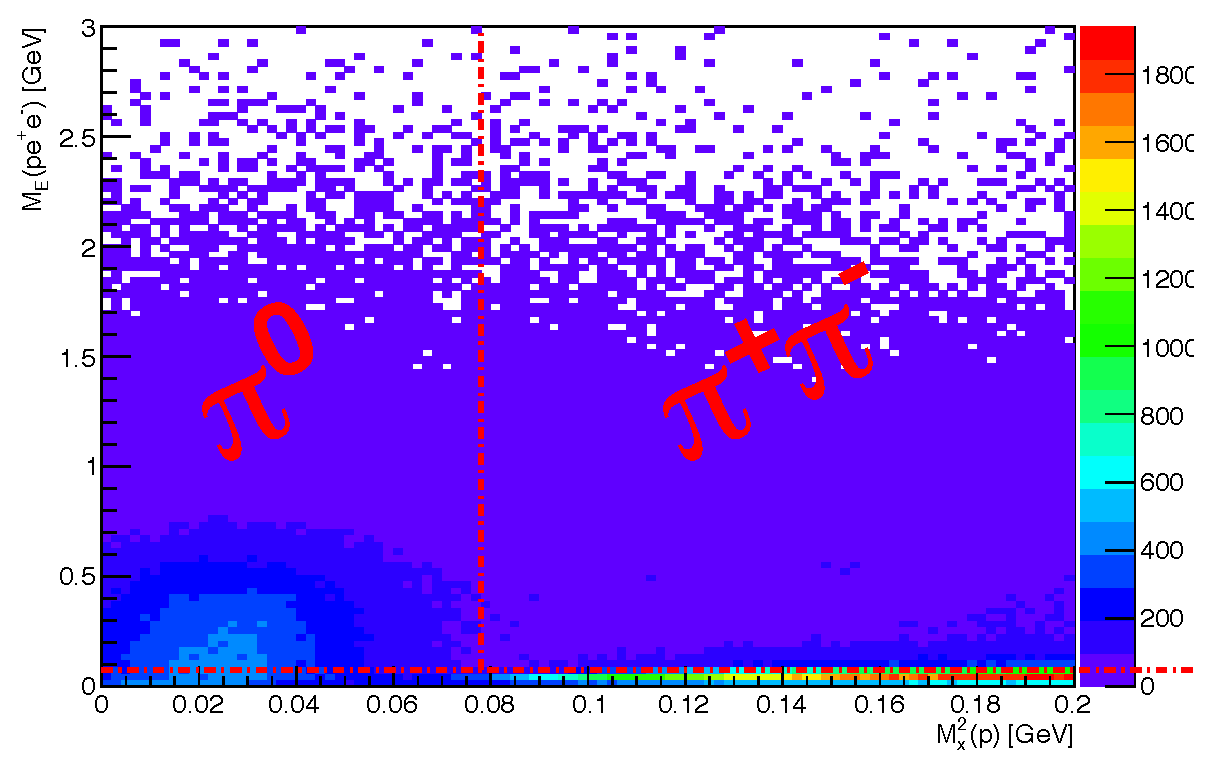
\includegraphics[width=0.8\figwidth]{\grpath/lepton/Lepfeature_cuts.eps}
			\caption[Cuts Applied to Isolate $\pi^0$ and $\pi^+\pi^-$ for PID Validation]{\label{fig:islep.cuts}Plot of missing mass squared of off proton (horizontal) vs. missing energy of proton $e^+e^-$ (vertical). The red dashed vertical line depicts the $\pi^+\pi^-$ threshold mass cut while the horizontal red dashed line represents the missing energy cut-off used to separate $\pi^+\pi^-$ from $\pi^0$. Image source:~\cite{thesiskunkel,g12note}}
\end{center}\end{figure}
%\begin{figure}[h!]\begin{center}
%		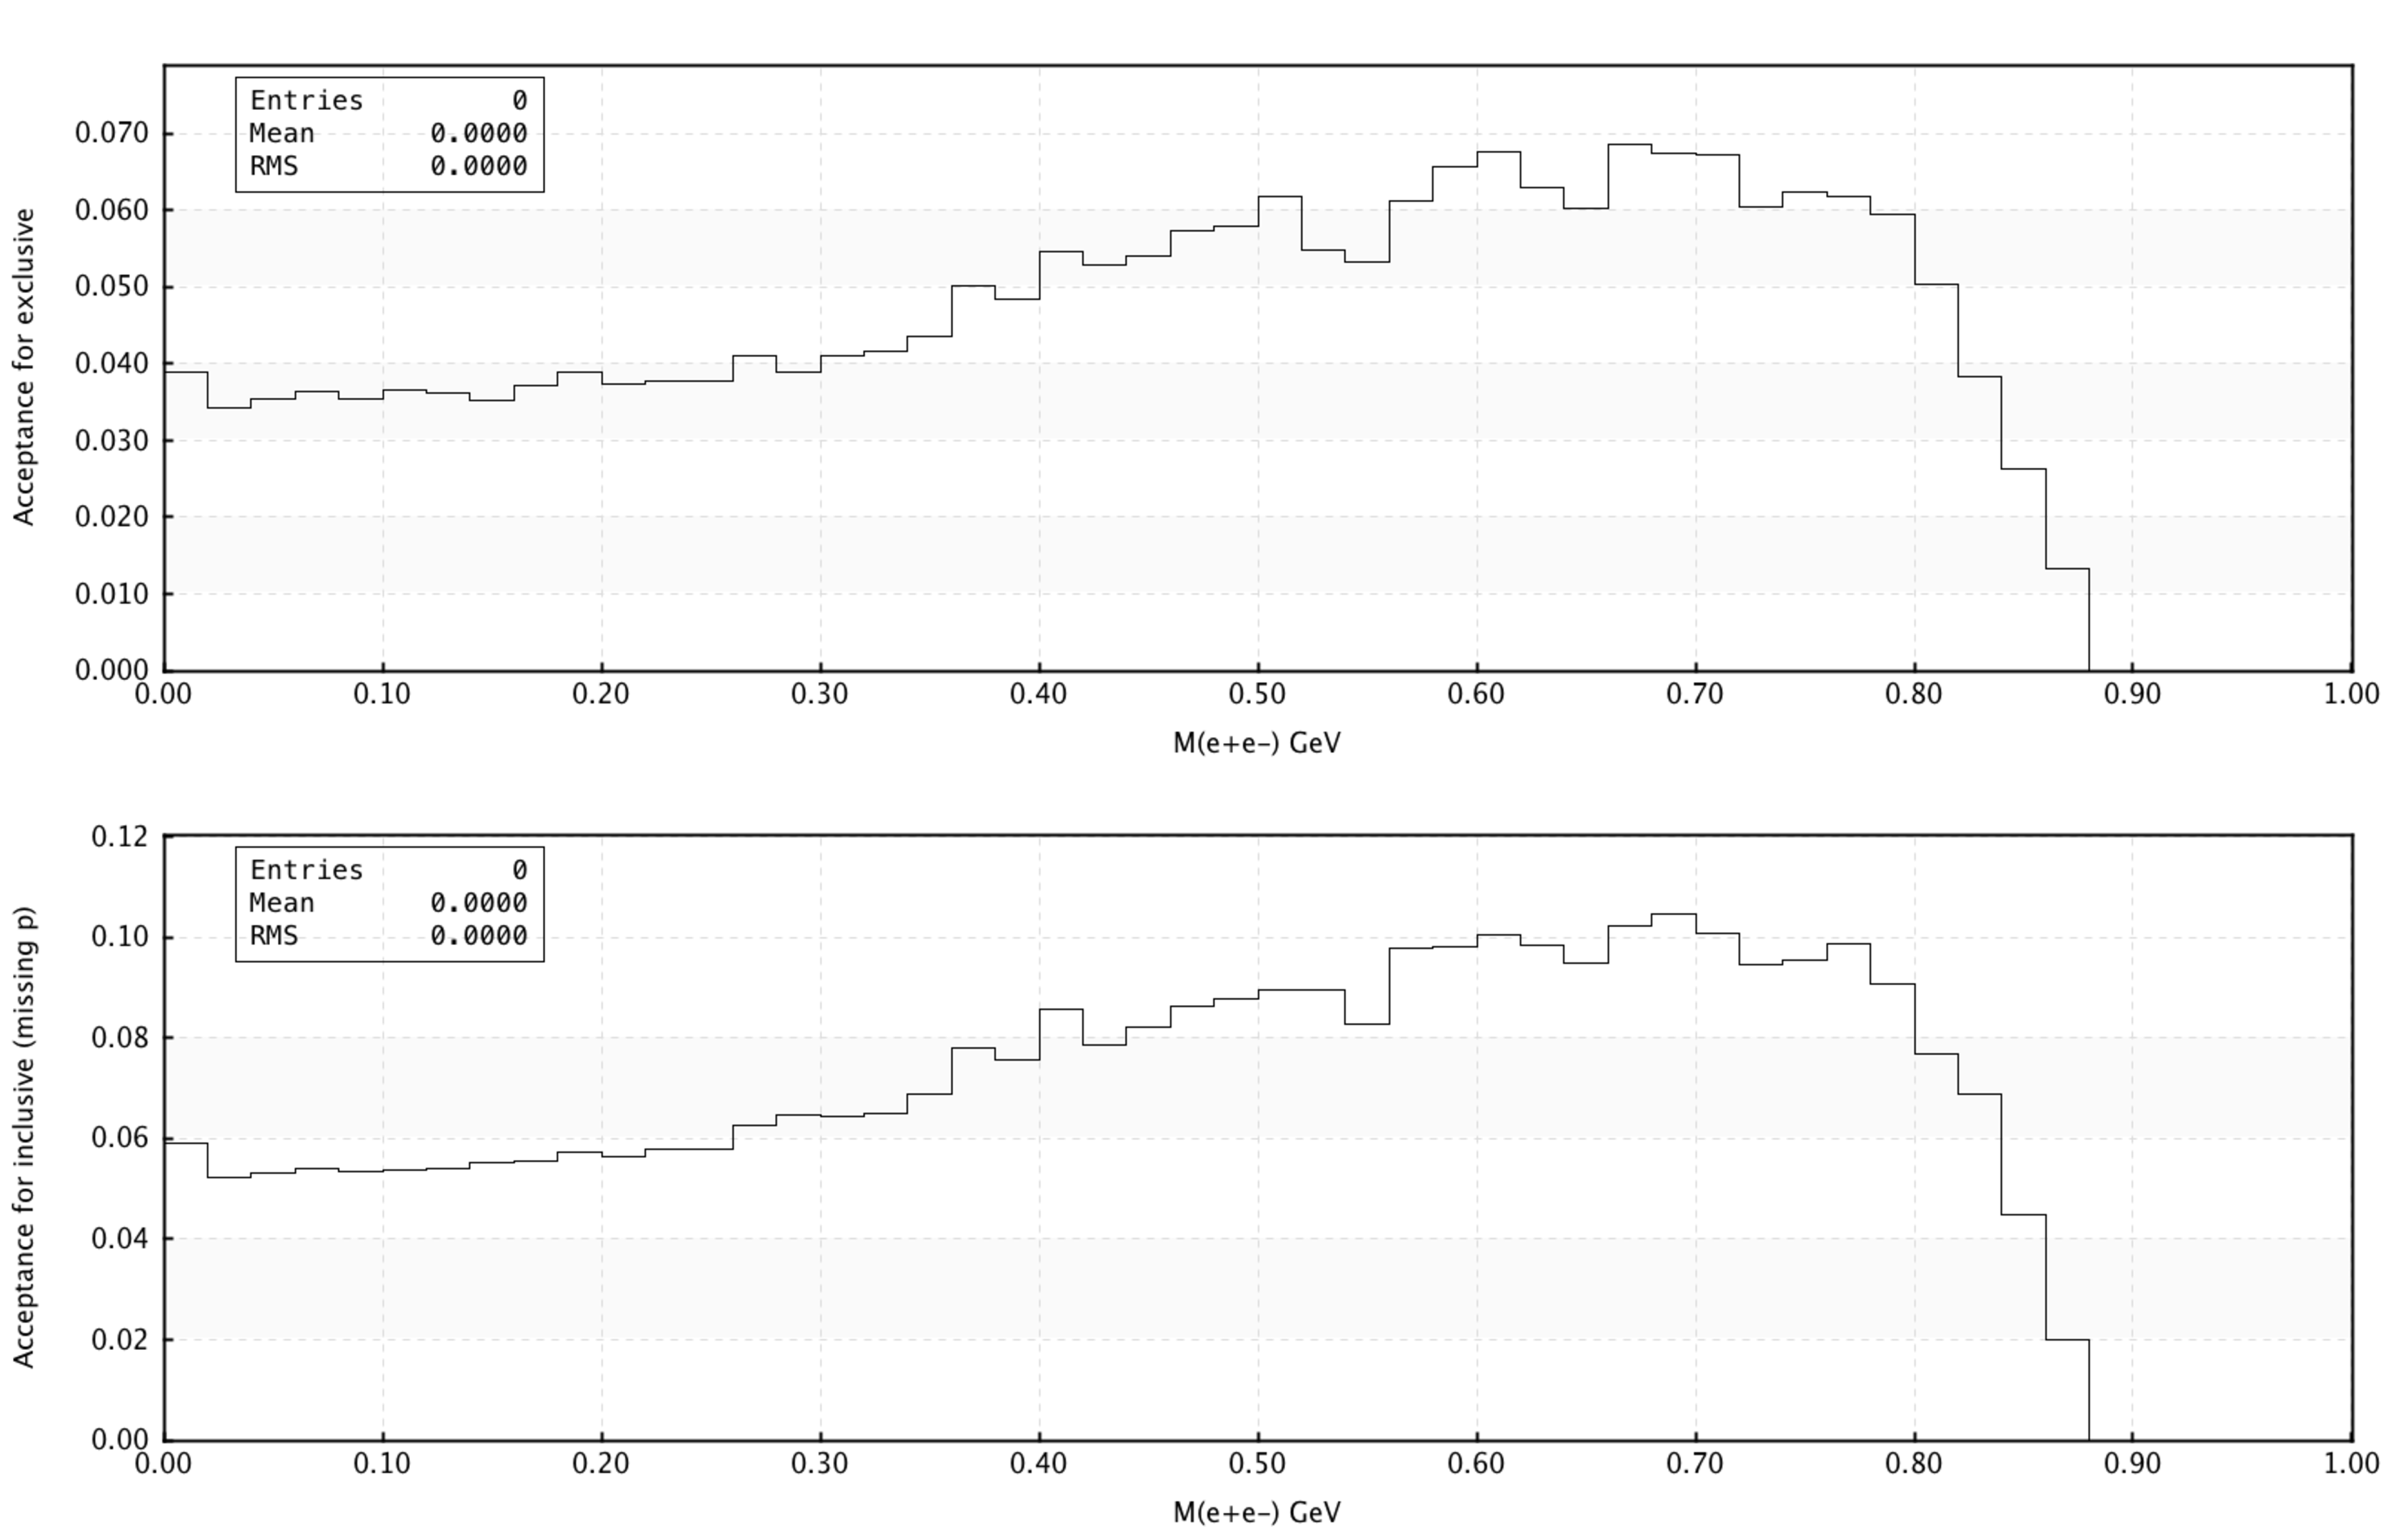
\includegraphics[width=\figwidth,height=1.2\qfigheight]{\grpath/counts/75_TORUS/VMD/VMD_Acceptance.pdf}
%		\caption[Acceptance, as a function of $M(\epem)$]{\label{fig:VMDaccepted}{Acceptance using a VMD decay model, as a function of $M(\epem)$ for the exclusive (Top) and inclusive reconstruction scheme(Bottom). }}
%	\end{center}\end{figure}		
\FloatBarrier
\paragraph{\label{sec:data.lepton.cc}CC Comparison}

The NPE measured by the CC for all positron/electron (e$^+$/e$^-$) candidates can be seen in Fig~\ref{fig:islep.CC}. The sharp decline prior to 2.5 NPE is due to photo-electrons created by electron/positrons, pions traveling through the CC or pions producing delta-electrons which pass through the CC. Delta-electrons are created as an effect of the ionization of gases that could be present when the pion travels through the DC. These types of electrons are typically lower in momentum than the electrons obtained from particle decays in CLAS and thus should emit less NPE per unit length.

Through mass conservation the particles for the $\pi^0$ events must be $e^+e^-$ pairs. In comparison to fig.~\ref{fig:islep.CC}, fig.~\ref{fig:islep.CC1} plots the NPE measured by the CC for all e$e^+e^-$ pairs for $\pi^0$ events selected as shown in fig.~\ref{fig:islep.cuts}. It can be seen that the sharp decline prior to NPE = 2.5 is reduced leaving mostly electrons or positrons signatures in the CC concluding that the g12 CC NPE cut is valid for identifying $e^+e^-$ pairs while rejecting $\pi^+\pi^-$ pairs.
Using the current cuts of NPE and hit angle, the suppression of di-leptons was sufficient without including additional cuts on the CC such as a timing comparison to the TOF.

%
\begin{figure}\begin{center}
		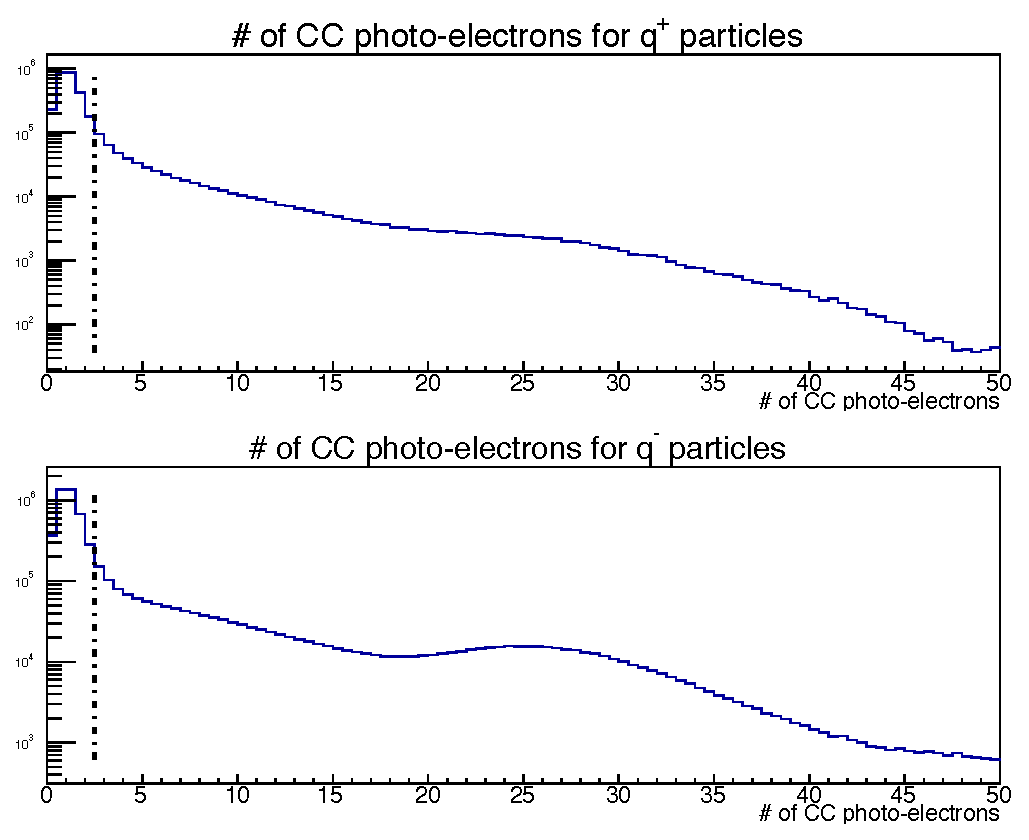
\includegraphics[width=0.8\figwidth]{figures/lepton/CC_nPE.eps}
		\caption[Number of Photo-electrons Measured by CC for All $e^-$ and $e^+$ Candidates]{\label{fig:islep.CC}Plot of NPE measured by CLAS CC subsystem for positron/electron candidates top/bottom respectively. The dashed dotted vertical line depicts the cut applied if using the g12 lepton PID scheme. Image source:~\cite{thesiskunkel}}
\end{center}\end{figure}
	
\begin{figure}\begin{center}
			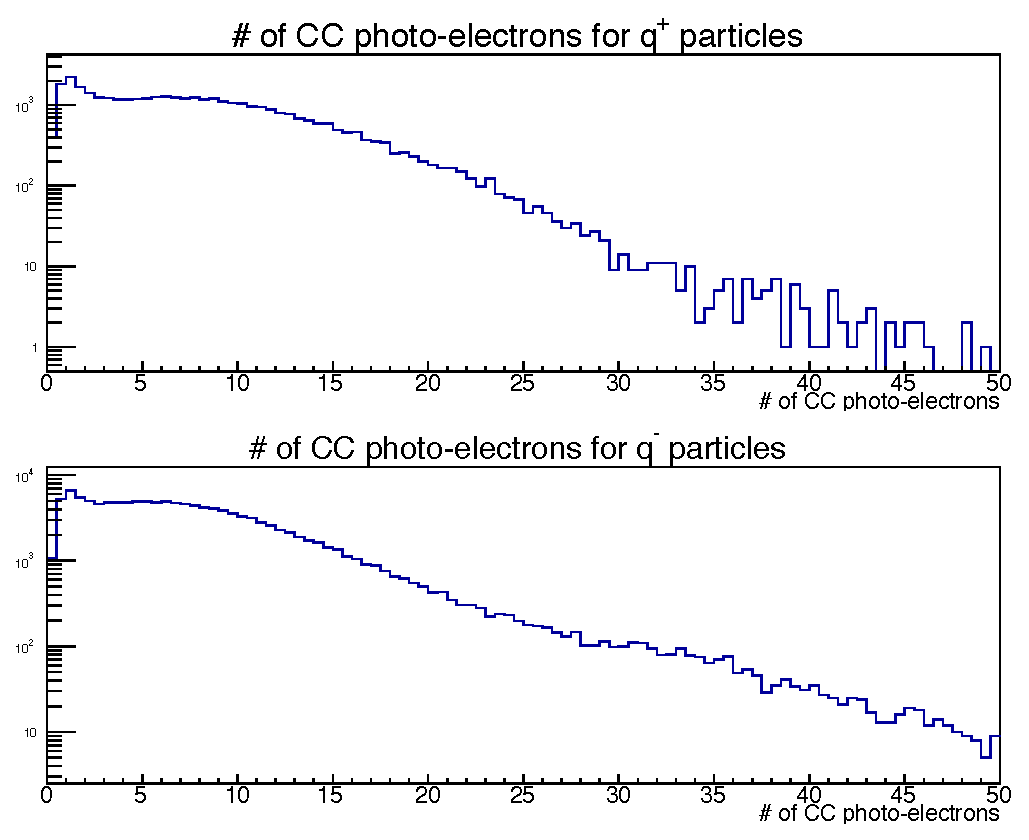
\includegraphics[width=0.8\figwidth]{figures/lepton/CC_NPEcut.eps}
			\caption[Number of Photo-electrons Measured by CC for $\pi^0$ Events]{\label{fig:islep.CC1}Plot of NPE measured by CLAS CC subsystem when selecting $\pi^0$ events seen in Fig~\ref{fig:islep.cuts}, positron/electron candidates top/bottom respectively. Image source:~\cite{thesiskunkel}}
\end{center}\end{figure}
		
\FloatBarrier

\paragraph{\label{sec:data.lepton.ec}EC Comparison}
		
		Similarly to the CC comparison, figures~\ref{fig:islep.pimEClow},~\ref{fig:islep.pimEChigh},~\ref{fig:islep.pipEClow},~\ref{fig:islep.pipEChigh} depict the  p$\mathrm{_{thres}^{low}}$ and  p$\mathrm{_{thres}^{low}}$ cuts listed in Tab.~\ref{tab:ISLEP_cuts} for the q$^-$ and q$^+$ tracks respectively. After $\pi^0$ event selection, seen in figures~\ref{fig:islep.pimEC},~\ref{fig:islep.pimECcut} ,~\ref{fig:islep.pipEC} ,~\ref{fig:islep.pipECcut}, the bulk of $e^+e^-$ events reside within the region of the cut acceptance therefore it is evident that the g12 EC cuts are valid for identifying \epemT \ pairs. The following four plots are for electron($e^-$) PID validation of the g12 EC cuts described in Tab.~\ref{tab:ISLEP_cuts}.
		%
\begin{figure}\begin{center}
				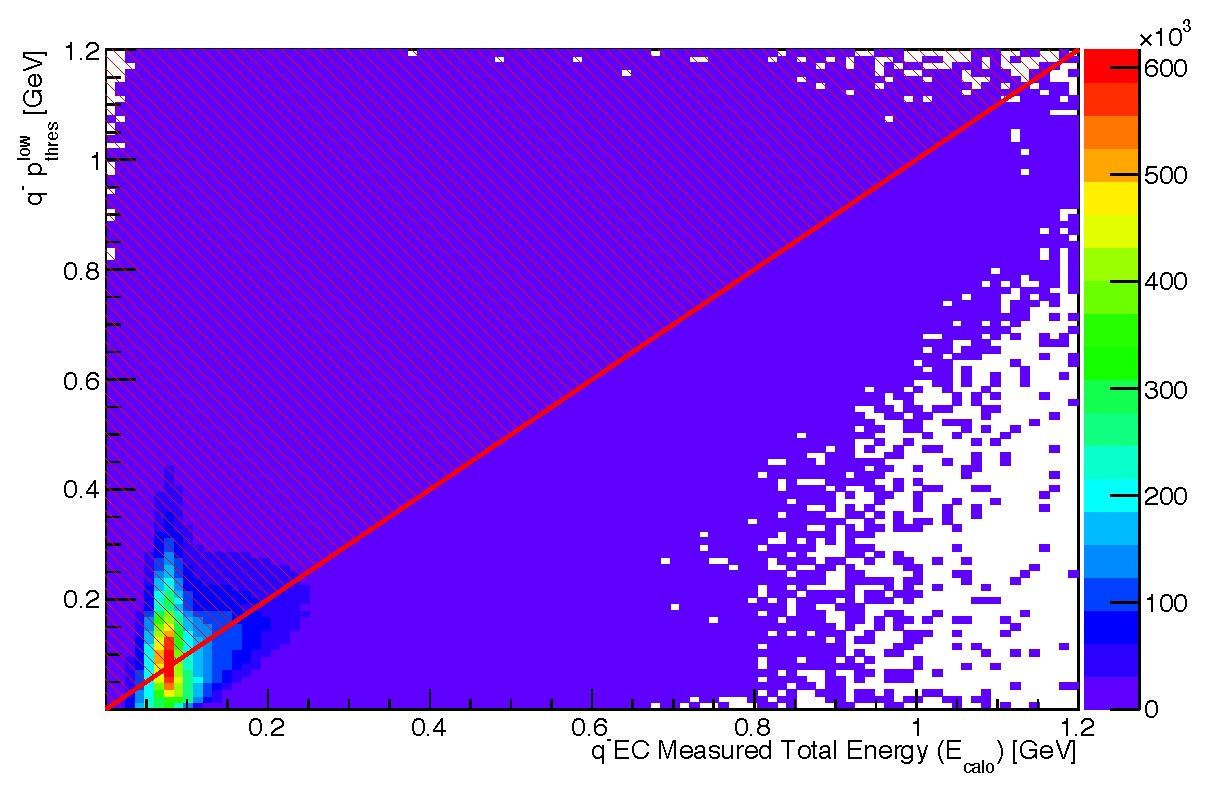
\includegraphics[width=0.8\figwidth]{figures/lepton/Pim_EClow.eps}
				\caption[EC Deposited Energy Comparison to Lower Threshold Track Momentum for q$^-$ Tracks]{\label{fig:islep.pimEClow}Plot of energy deposited measured by EC vs. track momentum p$\mathrm{_{thres}^{low}}$ for negative charged tracks. The red region depicts the cut that would reject events in the g12 lepton EC PID scheme. Image source:~\cite{thesiskunkel}}
\end{center}\end{figure}
			
\begin{figure}\begin{center}
					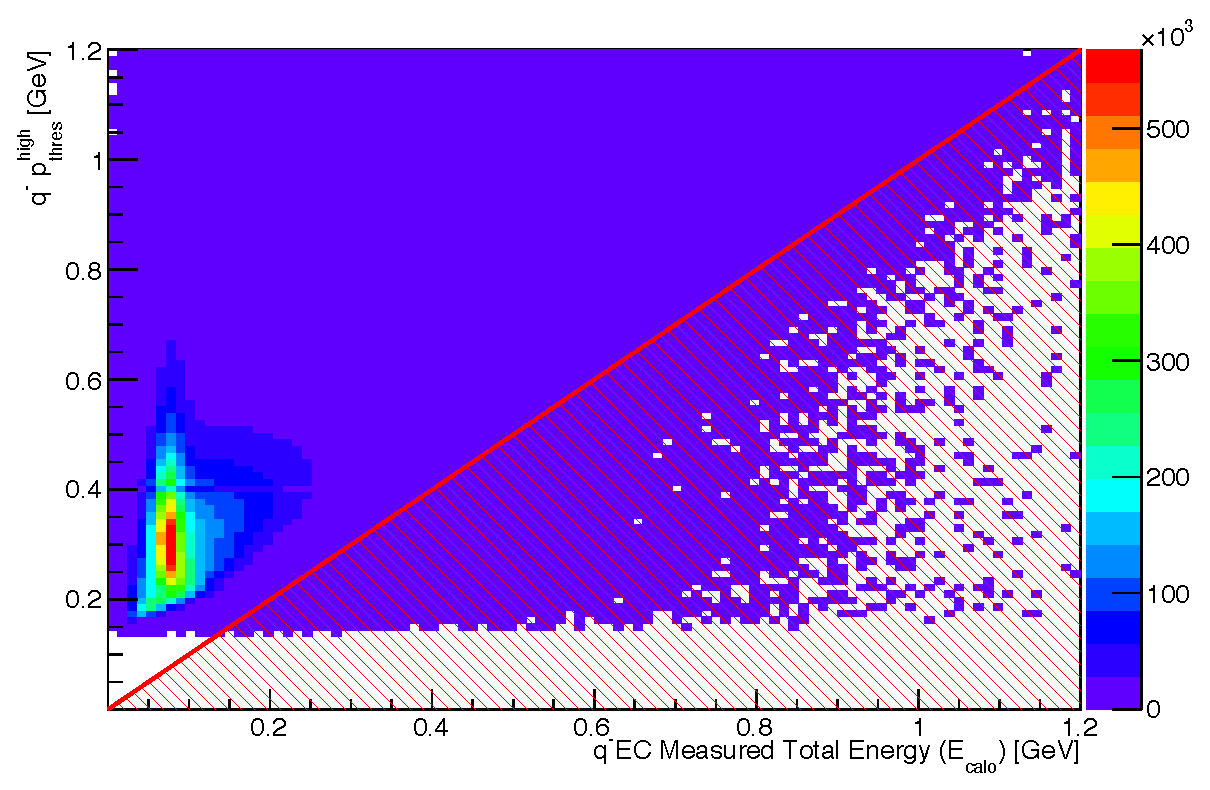
\includegraphics[width=0.8\figwidth]{figures/lepton/Pim_EChigh.eps}
					\caption[EC Deposited Energy Comparison to Upper Threshold Track Momentum for q$^-$ Tracks]{\label{fig:islep.pimEChigh}Plot of energy deposited measured by EC vs. track momentum p$\mathrm{_{thres}^{high}}$ for negative charged tracks. The red region depicts the cut that would reject events in the g12 lepton EC PID scheme. Image source:~\cite{thesiskunkel}}
\end{center}\end{figure}
				
				
\begin{figure}\begin{center}
						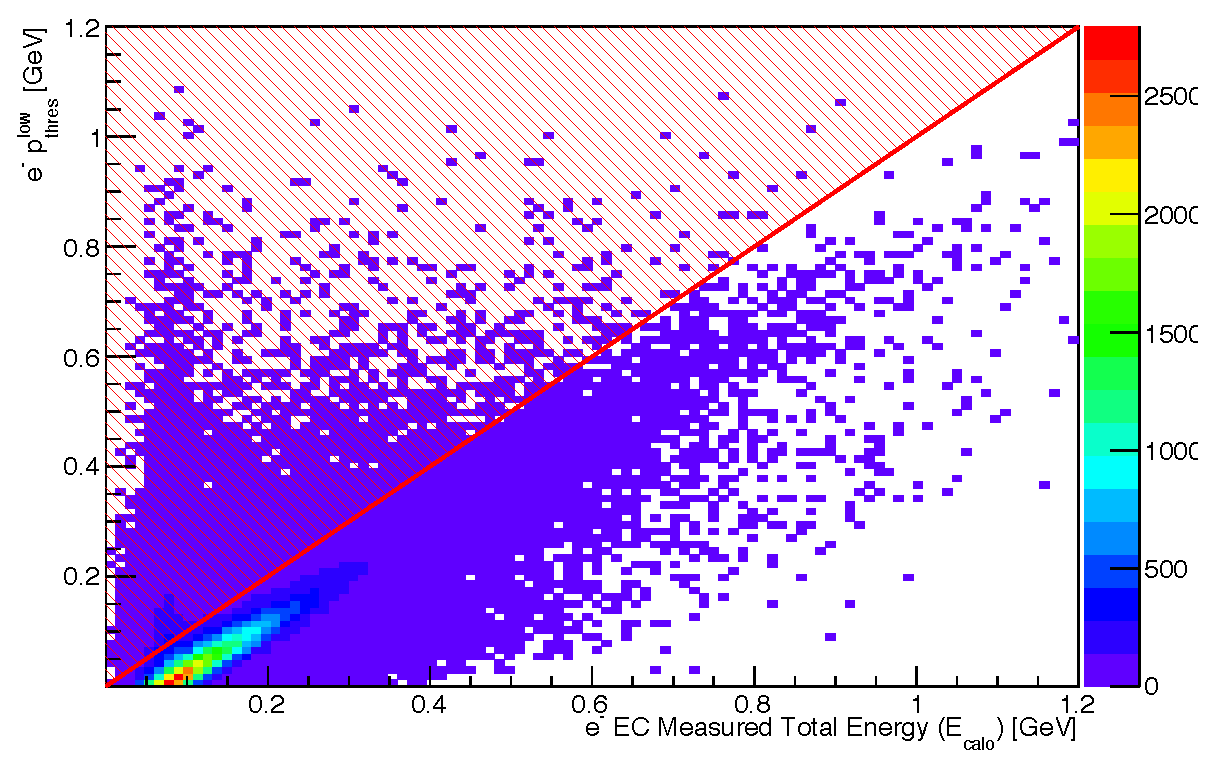
\includegraphics[width=0.8\figwidth]{figures/lepton/Pim_EClowcut.eps}
						\caption[EC Deposited Energy Comparison to Track Momentum for $e^-$ Candidates]{\label{fig:islep.pimEC}Plot of energy deposited measured by EC vs. track momentum p$\mathrm{_{thres}^{low}}$ for electrons from $\pi^0$ events without the g12 lepton EC PID scheme applied. The red region depicts the cut that would reject events in the g12 lepton EC PID scheme. Image source:~\cite{thesiskunkel}}
\end{center}\end{figure}
					
\begin{figure}\begin{center}
							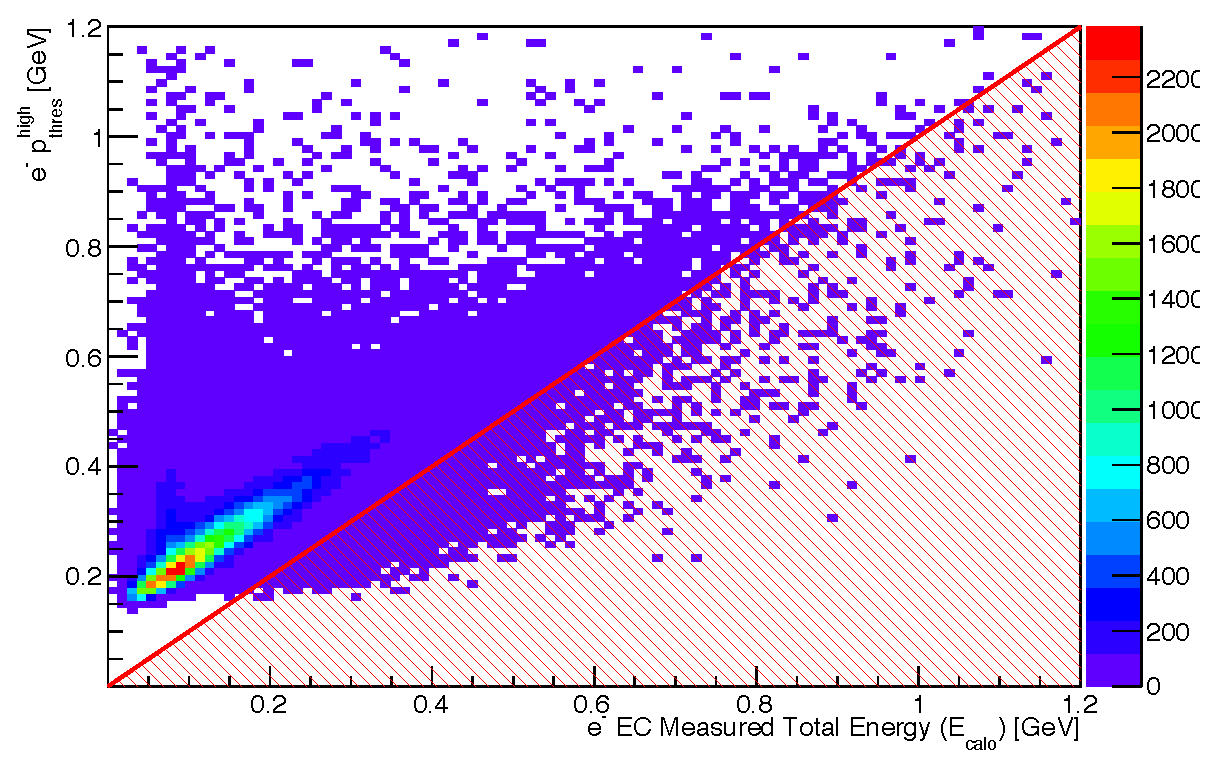
\includegraphics[width=0.8\figwidth]{figures/lepton/Pim_EChighcut.eps}
							\caption[EC Deposited Energy Comparison to Track Momentum for $e^-$ from $\pi^0$ Events]{\label{fig:islep.pimECcut}Plot of energy deposited measured by EC vs. track momentum p$\mathrm{_{thres}^{high}}$ for electrons from $\pi^0$ events without the g12 lepton EC PID scheme applied. The red region depicts the cut that would reject events in the g12 lepton EC PID scheme. Image source:~\cite{thesiskunkel}}
\end{center}\end{figure}
						
Figures~\ref{fig:islep.pipEClow}--\ref{fig:islep.pipECcut} are for positron ($e^+$) PID validation of the g12 EC cuts described in Tab.~\ref{tab:ISLEP_cuts}.
						
\begin{figure}\begin{center}
								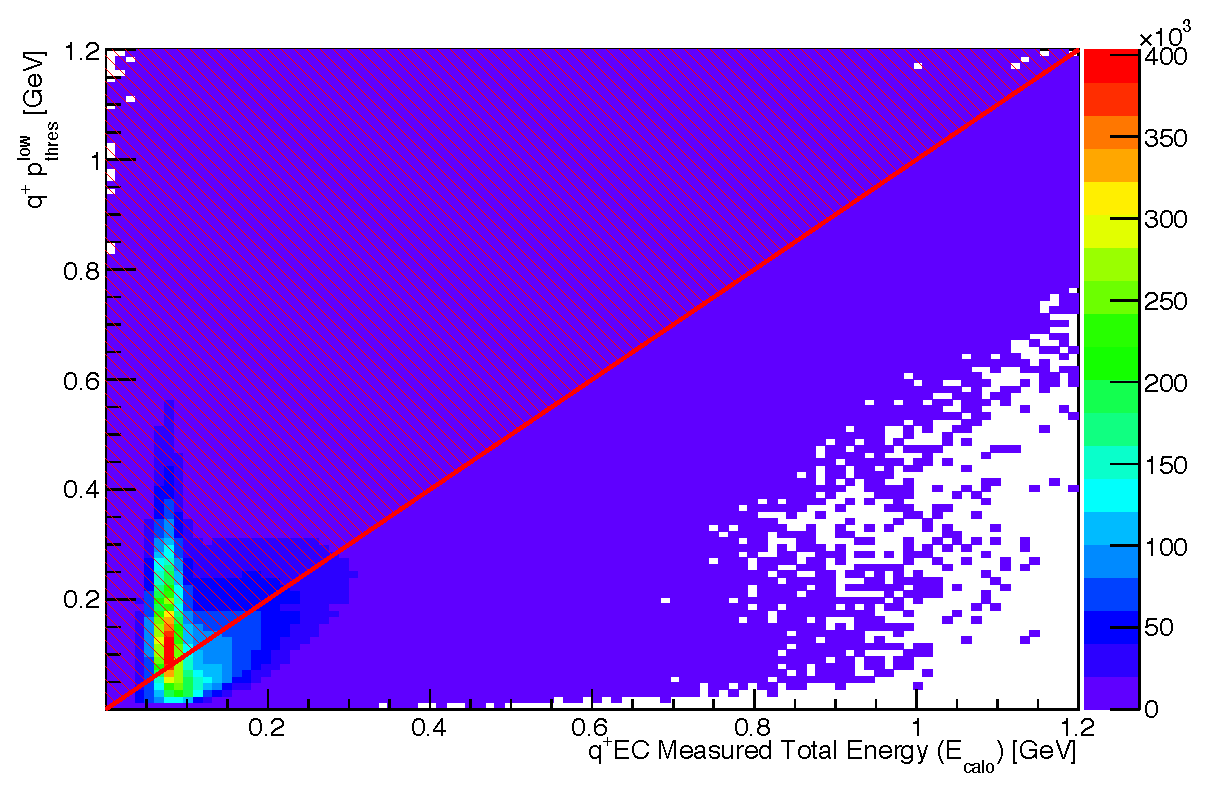
\includegraphics[width=0.8\figwidth]{figures/lepton/Pip_EClow.eps}
								\caption[EC Deposited Energy Comparison to Lower Threshold Track Momentum for q$^+$ Tracks]{\label{fig:islep.pipEClow}Plot of energy deposited measured by EC vs. track momentum p$\mathrm{_{thres}^{low}}$ for positive charged tracks. The red region depicts the cut that would reject events in the g12 lepton EC PID scheme. Image source:~\cite{thesiskunkel}}
\end{center}\end{figure}
							
\begin{figure}\begin{center}
									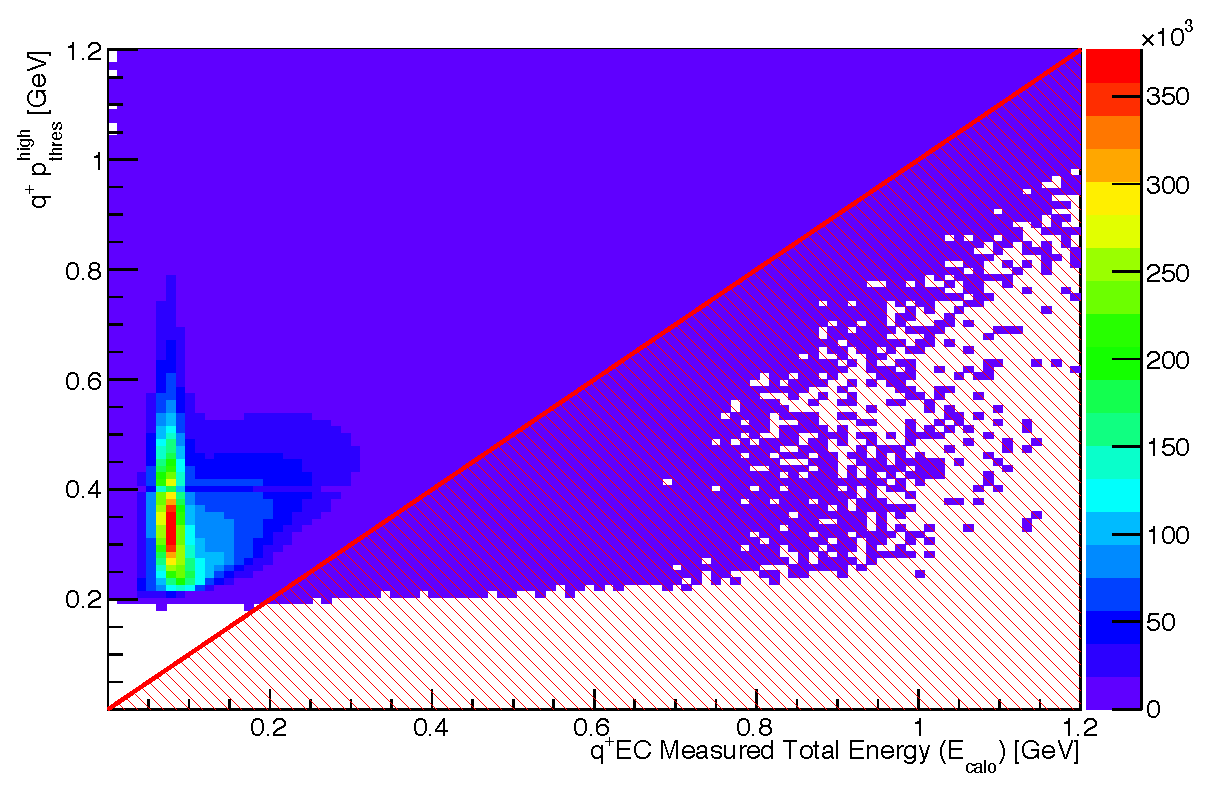
\includegraphics[width=0.8\figwidth]{figures/lepton/Pip_EChigh.eps}
									\caption[EC Deposited Energy Comparison to Upper Threshold Track Momentum for q$^+$ Tracks]{\label{fig:islep.pipEChigh}Plot of energy deposited measured by EC vs. track momentum p$\mathrm{_{thres}^{high}}$ for positive charged tracks. The red region depicts the cut that would reject events in the g12 lepton EC PID scheme. Image source:~\cite{thesiskunkel}}
\end{center}\end{figure}
								
\begin{figure}\begin{center}
										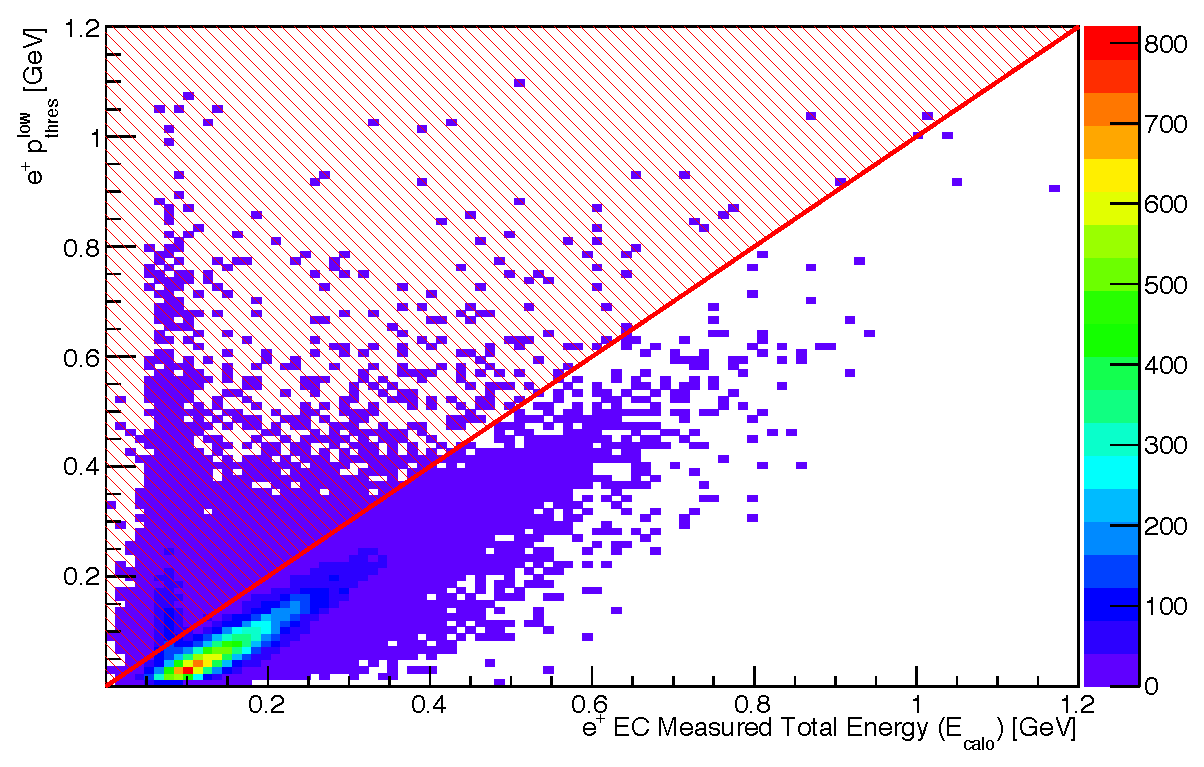
\includegraphics[width=0.8\figwidth]{figures/lepton/Pip_EClowcut.eps}
										\caption[EC Deposited Energy Comparison to Track Momentum for $e^+$ Candidates]{\label{fig:islep.pipEC}Plot of energy deposited measured by EC vs. track momentum p$\mathrm{_{thres}^{low}}$ for positrons from $\pi^0$ events without the g12 lepton EC PID scheme applied. The red region depicts the cut that would reject events in the g12 lepton EC PID scheme. Image source:~\cite{thesiskunkel}}
\end{center}\end{figure}
									
\begin{figure}\begin{center}
											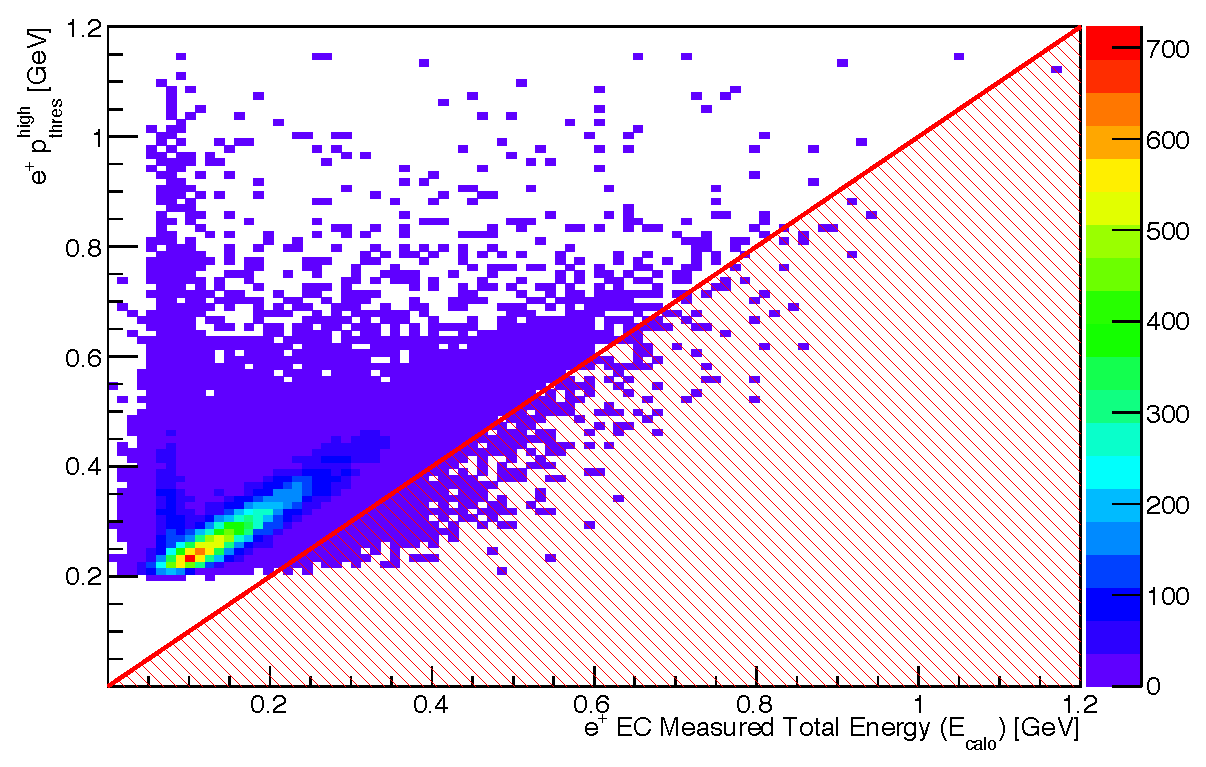
\includegraphics[width=0.8\figwidth]{figures/lepton/Pip_EChighcut.eps}
											\caption[EC Deposited Energy Comparison to Track Momentum for $e^+$ from $\pi^0$ Events]{\label{fig:islep.pipECcut}Plot of energy deposited measured by EC vs. track momentum p$\mathrm{_{thres}^{high}}$ for positrons from $\pi^0$ events without the g12 lepton EC PID scheme applied. The red region depicts the cut that would reject events in the g12 lepton EC PID scheme. Image source:~\cite{thesiskunkel}}
\end{center}\end{figure}																											
\FloatBarrier

%THIS IS THE PART I CHANGED
%=========================================================
\section{\etaPDal \  with CLAS g12}
The CLAS g12 vertex resolution was $\approx 10\,\mathrm{mm}$ (i.e. ten times larger than in the future CLAS12 apparatus) which was not suitable for a sufficient separation between external conversion and Dalitz events. However, the contamination from external conversion was only present in the low $M(\epem)$ mass bins.~\cite{thesisschever}.

\begin{figure}[h!]\begin{center}
  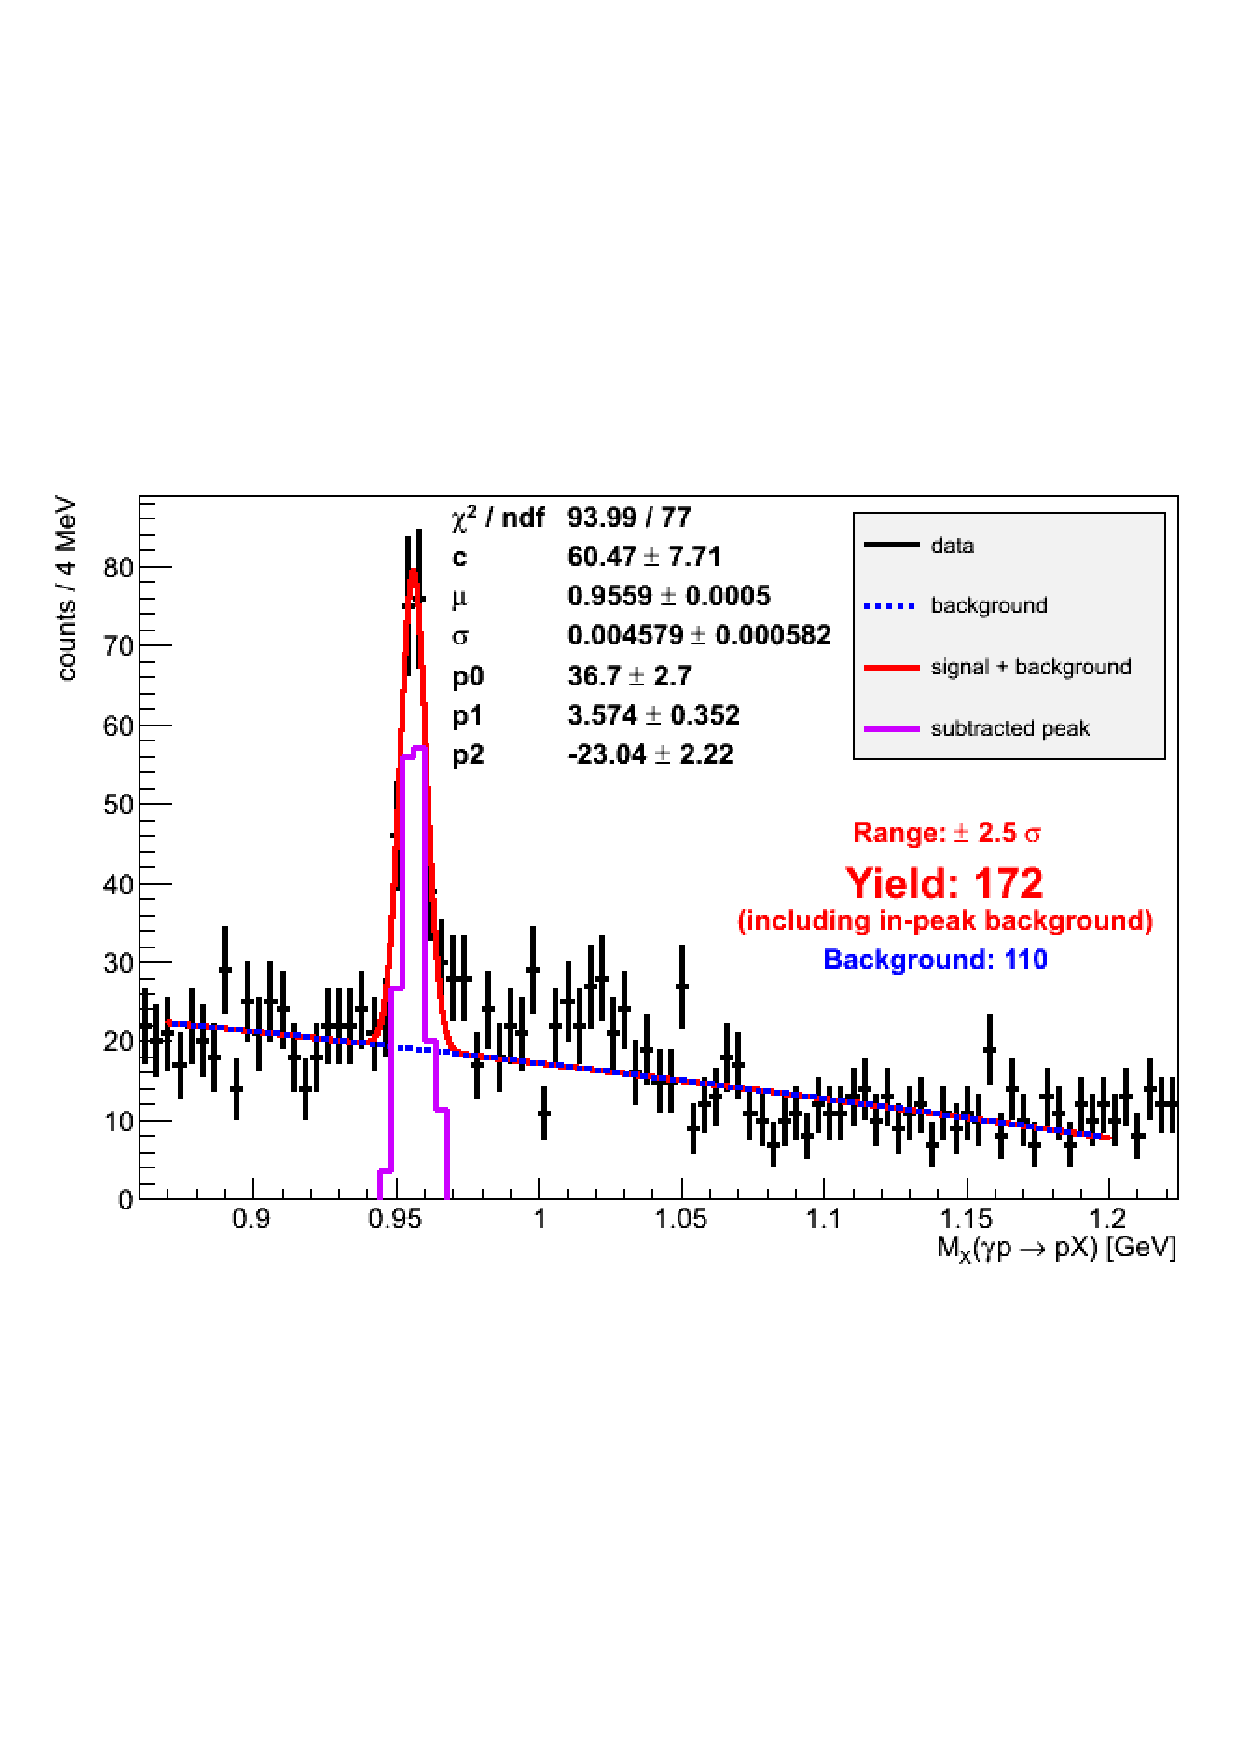
\includegraphics[width=0.8\textwidth]{etaPeeg_mimass.pdf}
  \label{fig:g12MxP}
  \caption[Counts rates for \etaTP from g12]{Missing mass of the proton for \etaPDal \  from CLAS g12.~\cite{thesisschever} The signal is fitted by a gaussian function whereas the background is fitted by a third order polynomial (blue curve). The sum of both, signal and background, is indicated by the red curve.}
\end{center}\end{figure}

Fig.~\ref{fig:g12MxP} shows the proton missing mass after reconstruction of  \etaPDal \  events in the CLAS g12 experiment.
 
%I AM NOT SURE HERE. THIS IS PURELY BASED ON MY EXPERIENCE WITH WASA:
The smooth background is related to direct neutral pion production, which either decay via a dalitz decay or two photons, where one photon produces a dilepton pair via external conversion. The predominant in-peak background contribution is related to the $\eta'\rightarrow \gamma\gamma$ decay.~\cite{thesisschever}.
The missing mass spectrum in Fig.~\ref{fig:g12Mxp} shows the need for a high statistics sample in order to be able to perform a side-band subtraction for the dilepton invariant mass spectrum.
%=========================================================
%	Using the Qfactor, signal to background separation, technique derived in CLAS~\cite{qfactor}, the total count rate of \etaPDal \ events detected in g12 was $\sim 89$. Figure~\ref{fig:g12figs} depicts the $\etaP$ signal extracted in g12 along with the $M(\epem)$ spectrum from the signal. 
%	\begin{figure}[h!]\begin{center}
%			\subfloat[$\etaP$ Dalitz and conversion spectra from g12][]{ %Feynman diagram of $\etaP$ two photon decay
%				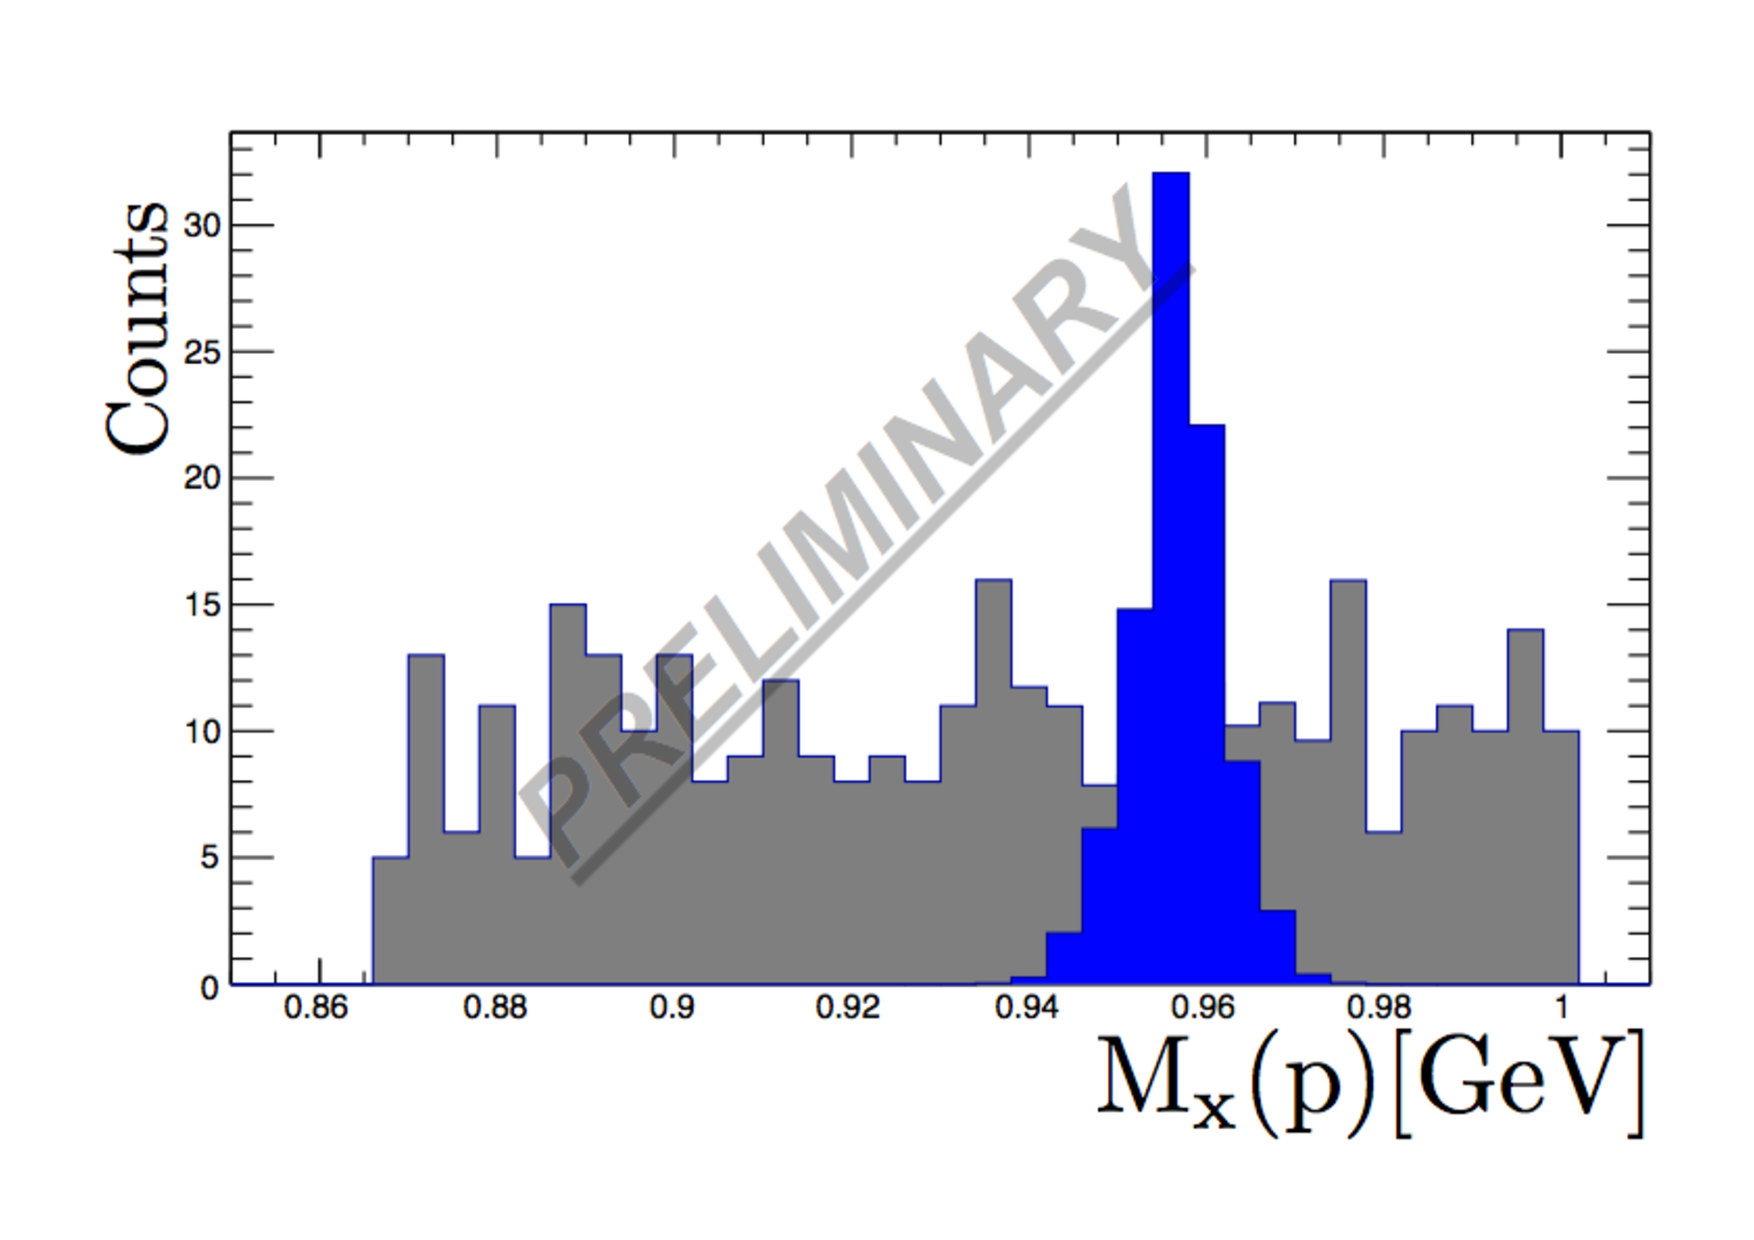
\includegraphics[width=0.8\columnwidth,height=1.0\qfigheight]{\grpath/g12/MxP_g12.pdf}\label{fig:g12MxP}
%			}
%			\\
%			\subfloat[$\phi$ Dalitz and conversion spectra from g12][]{ %Feynman diagram of $\etaP$ Dalitz decay
%				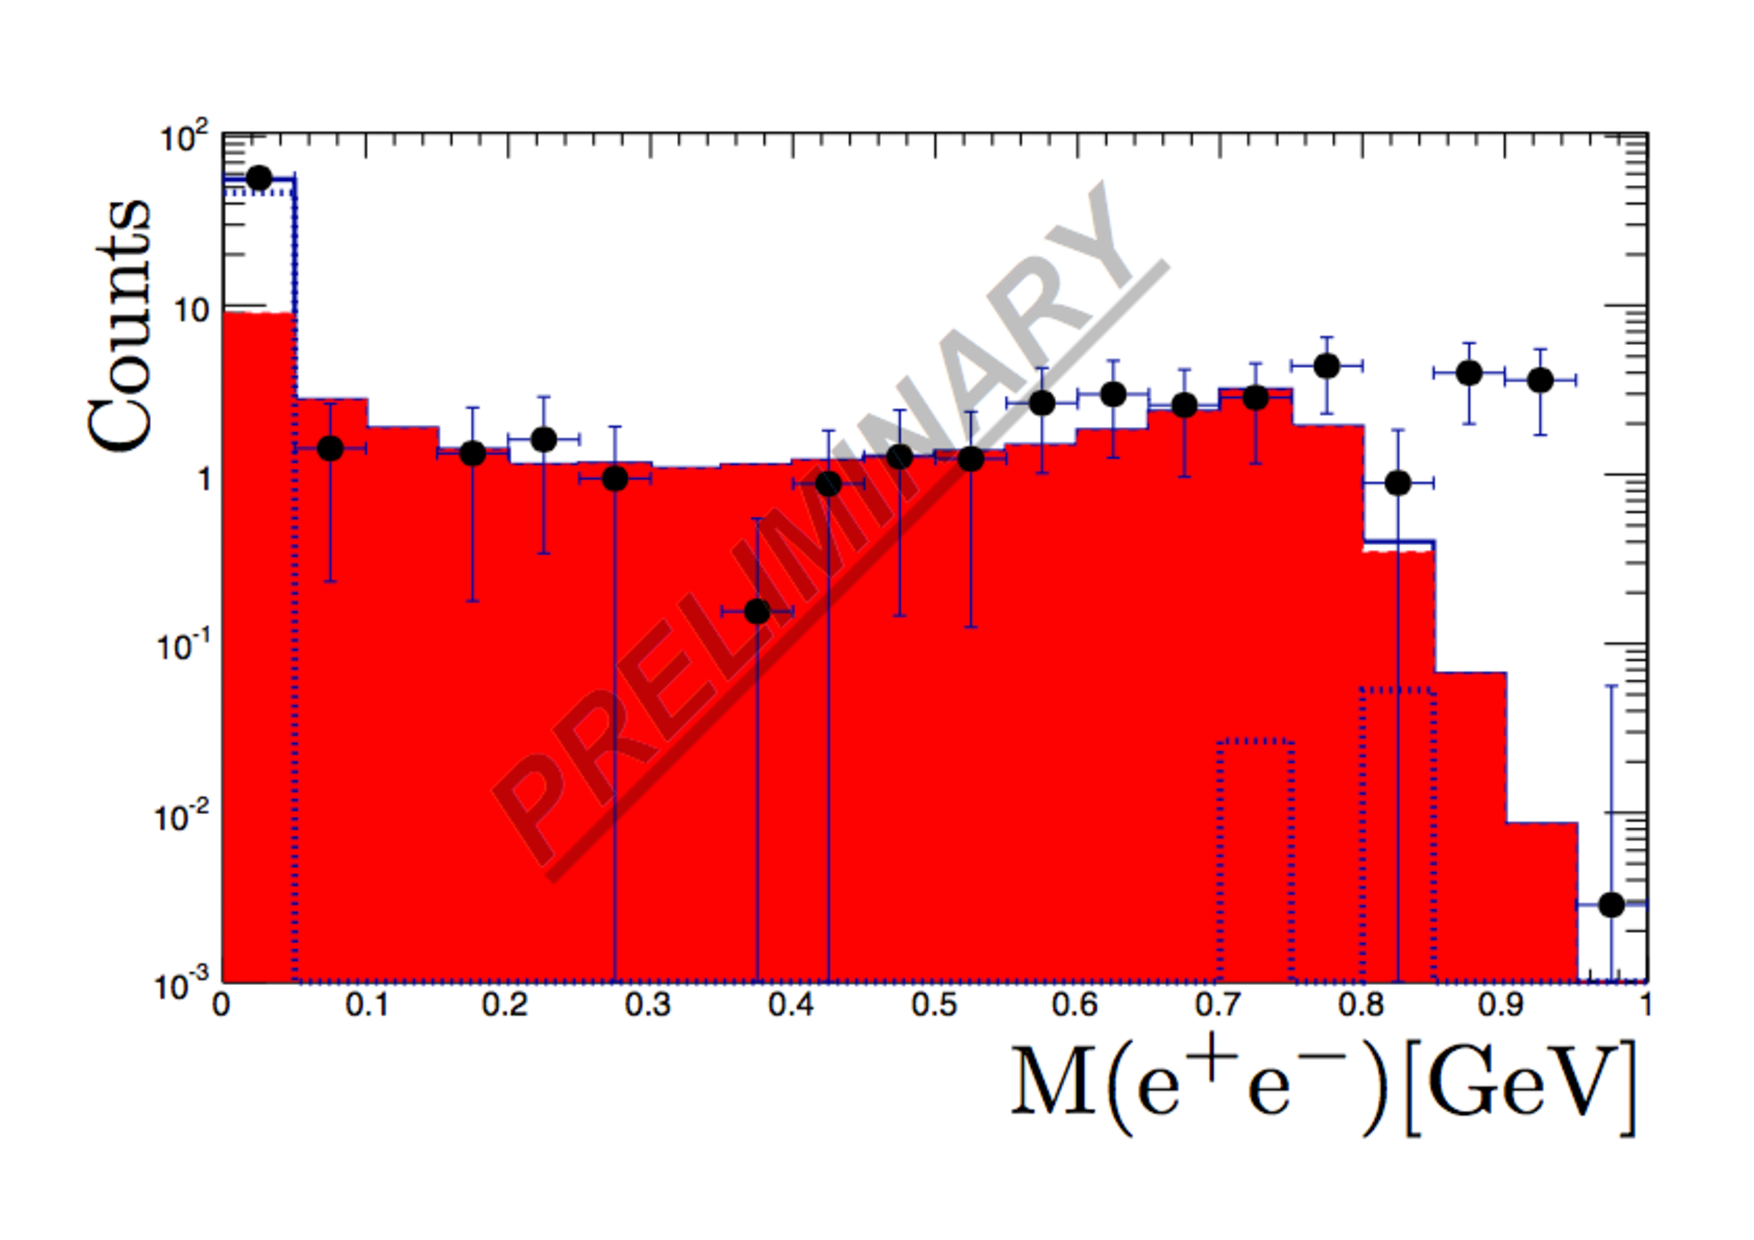
\includegraphics[width=0.8\columnwidth,height=1.0\qfigheight]{\grpath/g12/EpEm_g12.pdf}\label{fig:g12EpEm}
%			}
%			\caption[Counts rates for \etaTP from g12]{\label{fig:g12figs}~\subref{fig:g12MxP} Missing mass off of the proton for \etaPDal \  from CLAS g12. Q-factor weighted(Blue), Background (Grey). ~\subref{fig:g12EpEm} Invariant mass spectrum of \epemT \ under the blue curve in~\subref{fig:g12MxP}. Total counts in 29 days $\sim$ 89.}
%		\end{center}\end{figure}
%		\FloatBarrier 	
%		As seen in Fig.~\ref{fig:g12figs} the current CLAS results suffer from insufficient statistics. Therefore, we propose to repeat the \etaPDal \  measurement with CLAS12.
		\FloatBarrier
\section{Measurement}\label{sec:measurement}
This section is a description on how the \etaDal \ was simulated and reconstructed for this CLAS12 proposal.
\subsection{Simulation and Reconstruction}
To simulate the reaction in Eq.~\ref{eq:etaP}, the program PLUTO++~\cite{PLUTO} was utilize for its ability to simulate the decays of those according to QED, Vector Meson Dominance or a user defined TFF. For reconstruction of the desired topologies, the CLAS12 FASTMC~\cite{fastmc} was used, in which $\sim 5\cdot10^8$ events were generated for \etaPDal \ and then simulated with FASTMC at 75\% torus field. The efficiency for all detectors are assumed to be 100\% and only the geometric acceptance is considered for this proposal. Therefore the numbers that will be quoted in this proposal will be only an upper limit. An extra FASTMC simulation was performed for the torus field setting of 100\% to show the effects of the magnetic field on the lepton acceptance. 
%The EC efficiency  was calculated by comparing GEMC (GEANT4) simulations with FASTMC. This EC efficiency was also calculated with the g12 data set and was identical to the comparison of the two simulation methods.
 \newline
\indent The production of \etaTP \ was weighted by photo-production differential cross-sections, $\frac{d\sigma}{d\Omega}(v,\cos\theta_{cm})$, published in~\cite{Williams}, and $Q^2$. Where $v$ is the virtual photon energy, $\cos\theta_{cm}$ is the production angle in the center-of-mass frame of the system and $Q^2$, the production virtual photon, is defined as $-(k-k')^2$. This was done to achieve a quasi realistic model of the production. The \epemT \  decay spectrum, of each meson, was weighted via the VMD model (including QED predictions). Another simulation was performed using a flat $M(\epem)$ distribution (No QED, No VMD) to analyze any effects of the model on the \epemT acceptance. The analysis showed that the acceptance, in $M(\epem)$, was independent of the decay model, see Fig.\ref{fig:VMDaccepted} and Fig.\ref{fig:FLATaccepted}.
\subsubsection{Trigger Requirements}
The standard CLAS12 electron trigger (HTCC(Nphe>2) * [ (PCAL+EC)>1.0 GeV ] is sufficient for this types of analysis. The rate for hadron production in electro-production where the scattered electron is left undetected is $\sim 140\,\rm{kHz}$~\cite{Sargsyan}. This rate needs to be scaled down by the ratio of hardon production cross-section to \etaTP \ production cross-section, see Eq.~\ref{XsecR} in Sec.~\ref{sec:yield}. This ratio was calculated $\sim\frac{1}{200}$, which leads to an overall rate of 0.7~kHz, while the expected data acquisition (DAQ) readout rate is 10~kHz.
\subsubsection{Detection of \epemT Events} 
Electron/positron ID will include responses from the HTCC, PCAL and EC calorimeters. The energy information of the PCAL and the inner and outer parts of EC will be used to compare the total energy deposition with the momentum measured in the DC ($\alpha*(\mathrm{E_{Pcal}} + \mathrm{E_{ECin}}+ \mathrm{E_{ECout}}) \sim \mathrm{P_{DC}}$), where $\alpha$ is a scaling factor.
\subsubsection{Particle Identification}
The $\etaP$ meson have pion decay modes, which are orders of magnitude greater than the Dalitz decay. For example, the ratio $\Gamma_{\pi^+\pi^-\gamma} / \Gamma_{e^+e^- \gamma} $ is $ 6.2\cdot 10^2$. 
Electrons/positrons will be identified by using the information from the detectors described above. The expected $e^\pm/\pi^\pm$ rejection factor for single particles (p<4.9~GeV) is $10^3$ for the HTCC, while the PCAL+EC can provide an additional factor of $10^2$. Combining both methods yields a $e^\pm/\pi^\pm$ rejection factor of $10^5$ which results in a $e^+e^-/\pi^+\pi^-$ rejection factor of $10^{10}$. Therefore, the amount of $\pi^+\pi^-$ background in the $M(\epem)$ spectrum will be $\approx 6.2\cdot 10^2/10^{10} = 6.2\cdot10^{-8}$. A detailed explanation of particle identification for \epemT \ pairs can be found in~\cite{clas.proposal.jpsi}.
\subsubsection{Acceptance}\label{sec.reconstruction}
An inclusive reconstruction scheme
\begin{align}
ep\to e'p \etaP \rightarrow p e^+ \gamma e^- (e^-)
\end{align}
where a proton, a photon, a positron and one electron of unknown source is detected. It will be determined from kinematics which electron corresponds to the beam scattered electron or the Dalitz produced electron. 
\todo{Add daniels plots}
The acceptance was calculated by dividing the accepted events by the generated events, per $M(\epem)$ bin. The $\etaP$ Dalitz decay acceptance using the VMD as a decay model can be seen in Fig.\ref{fig:VMDaccepted}, while the acceptance using a flat \epemT \ mass distribution can be seen in Fig.~\ref{fig:FLATaccepted}. A comparison of these two figures shows a model independent \epemT \ acceptance. 
%\begin{figure}[h!]\begin{center}
%		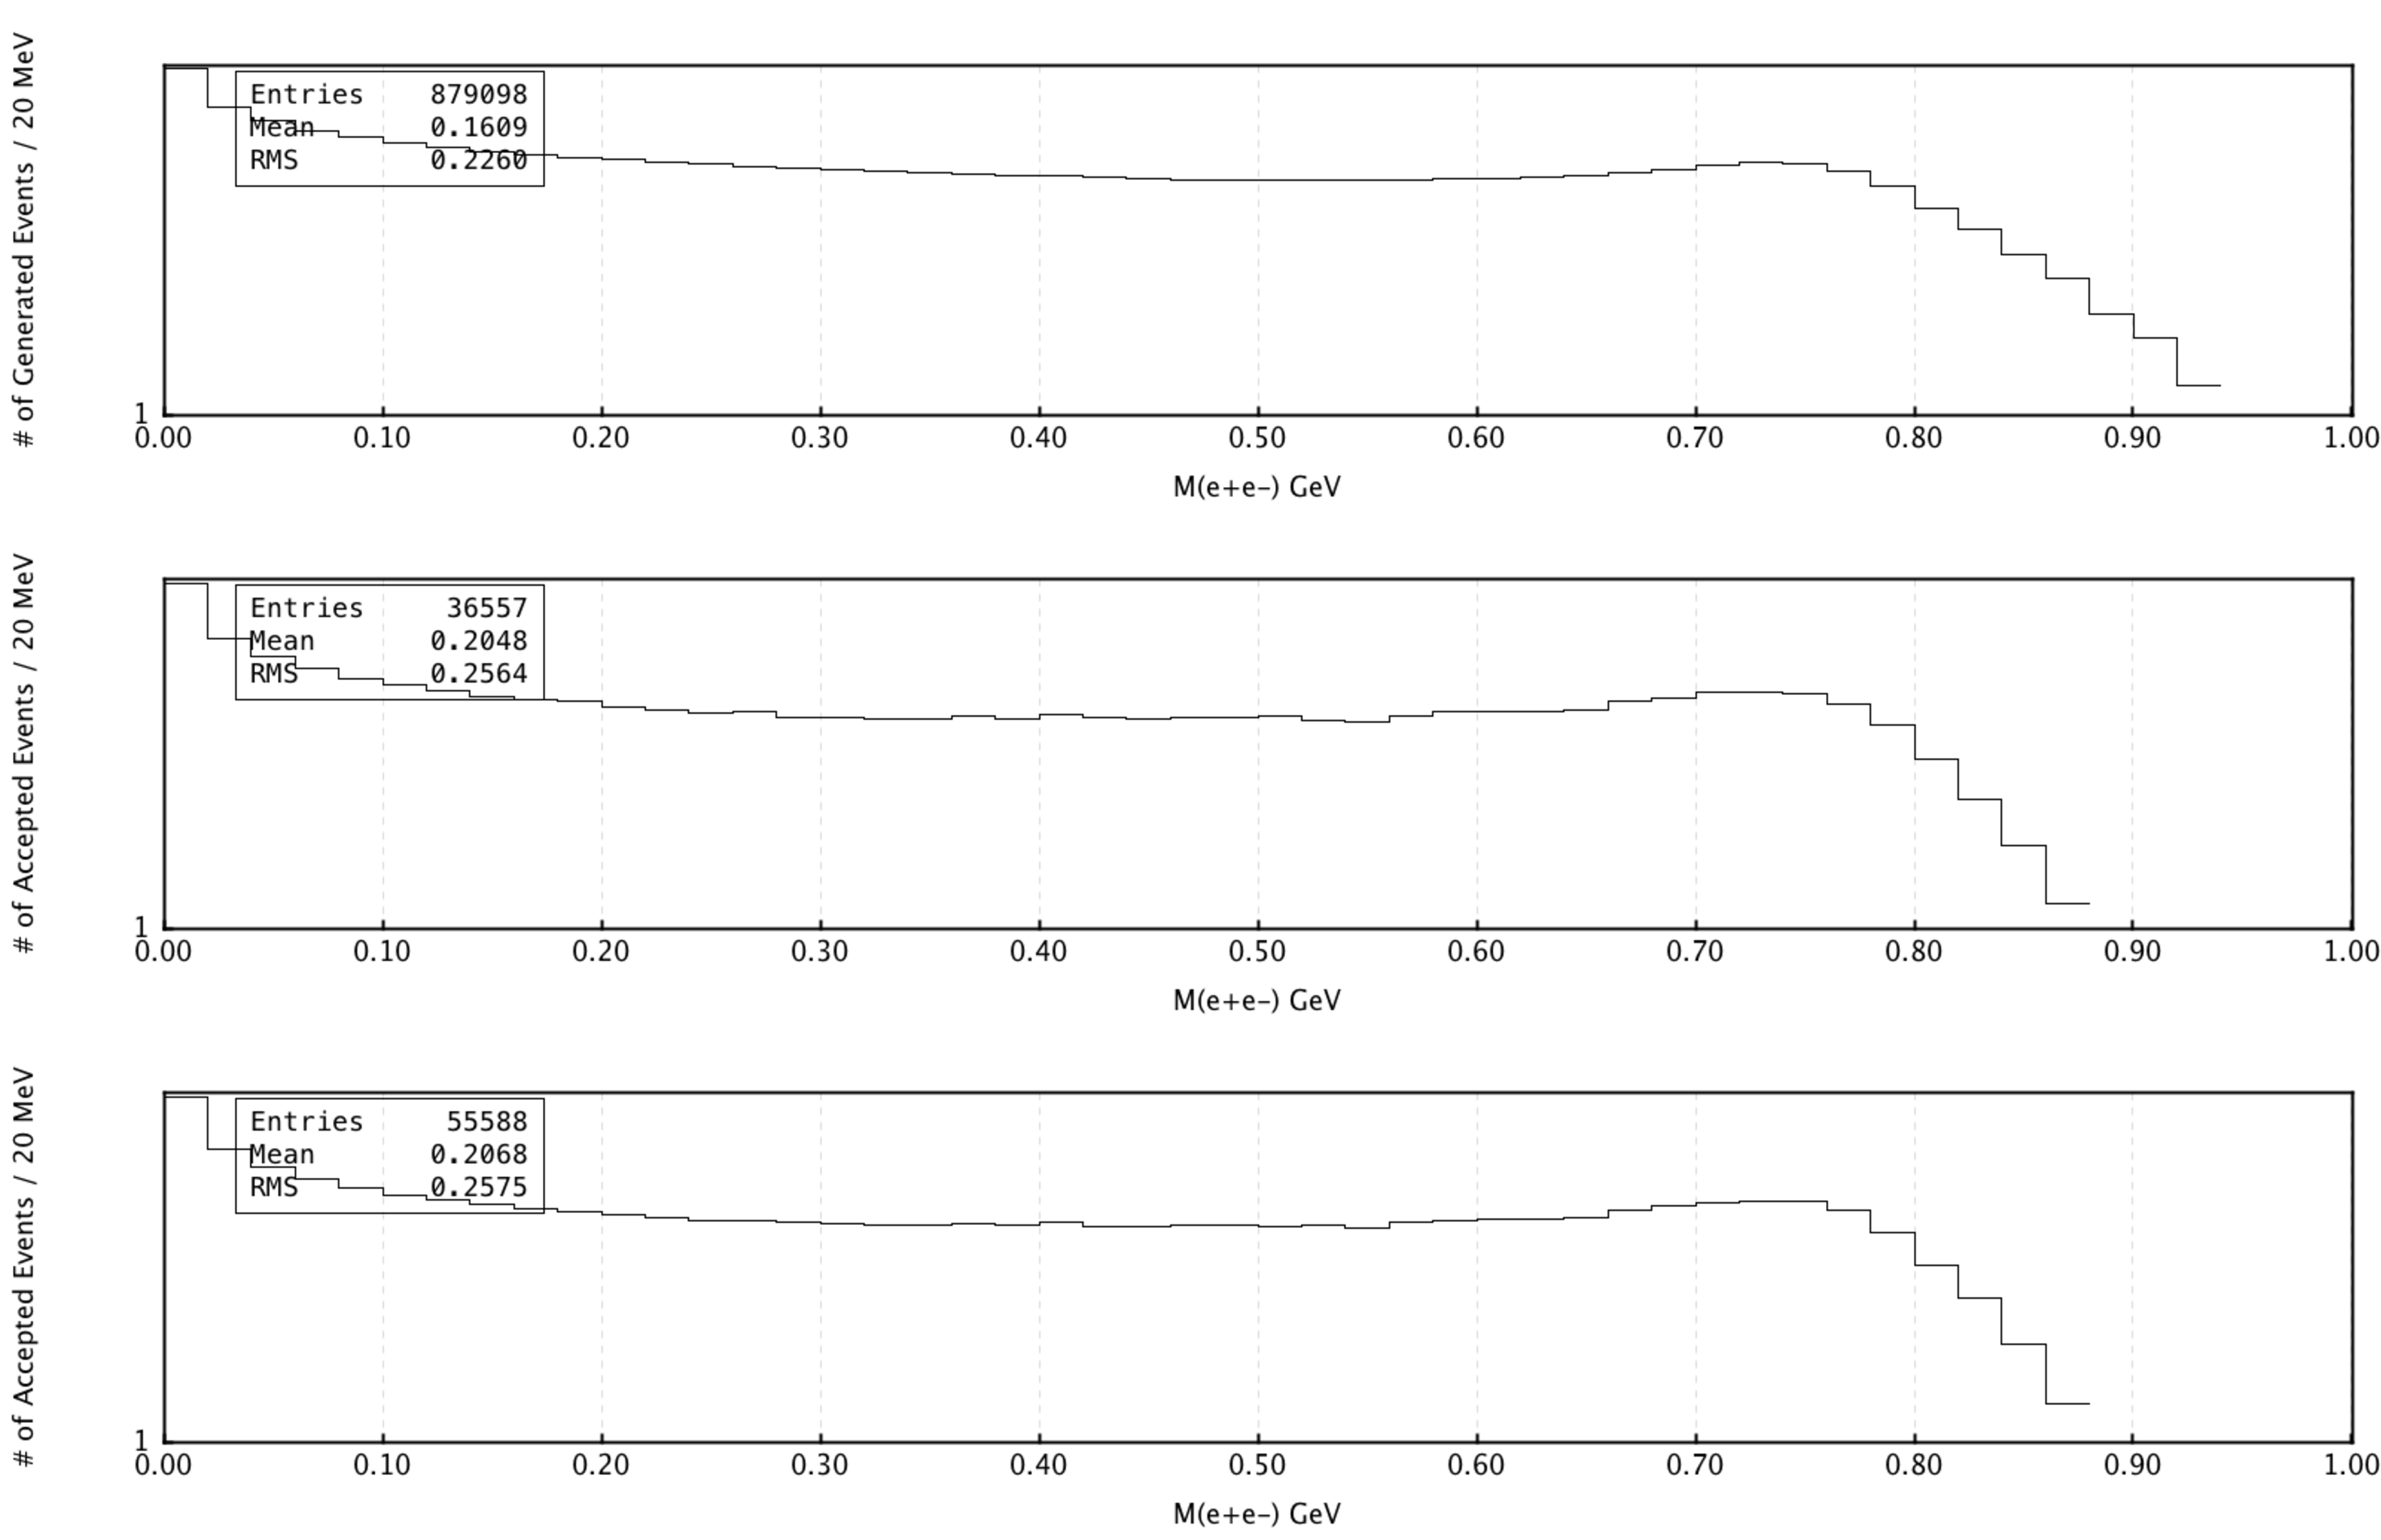
\includegraphics[width=\figwidth,height=2.6\qfigheight]{\grpath/counts/75_TORUS/VMD/VMD_Generated_Accepted.pdf}
%		\caption[Generated and Accepted counts, as a function of $M(\epem)$]{\label{fig:VMD}{Generated events (Top), accepted events for an exclusive (Middle), inclusive(Bottom) reconstruction schemes as a function of $M(\epem)$. In all panels a VMD decay model was employed}}
%\end{center}\end{figure}
%\begin{figure}[h!]\begin{center}
%			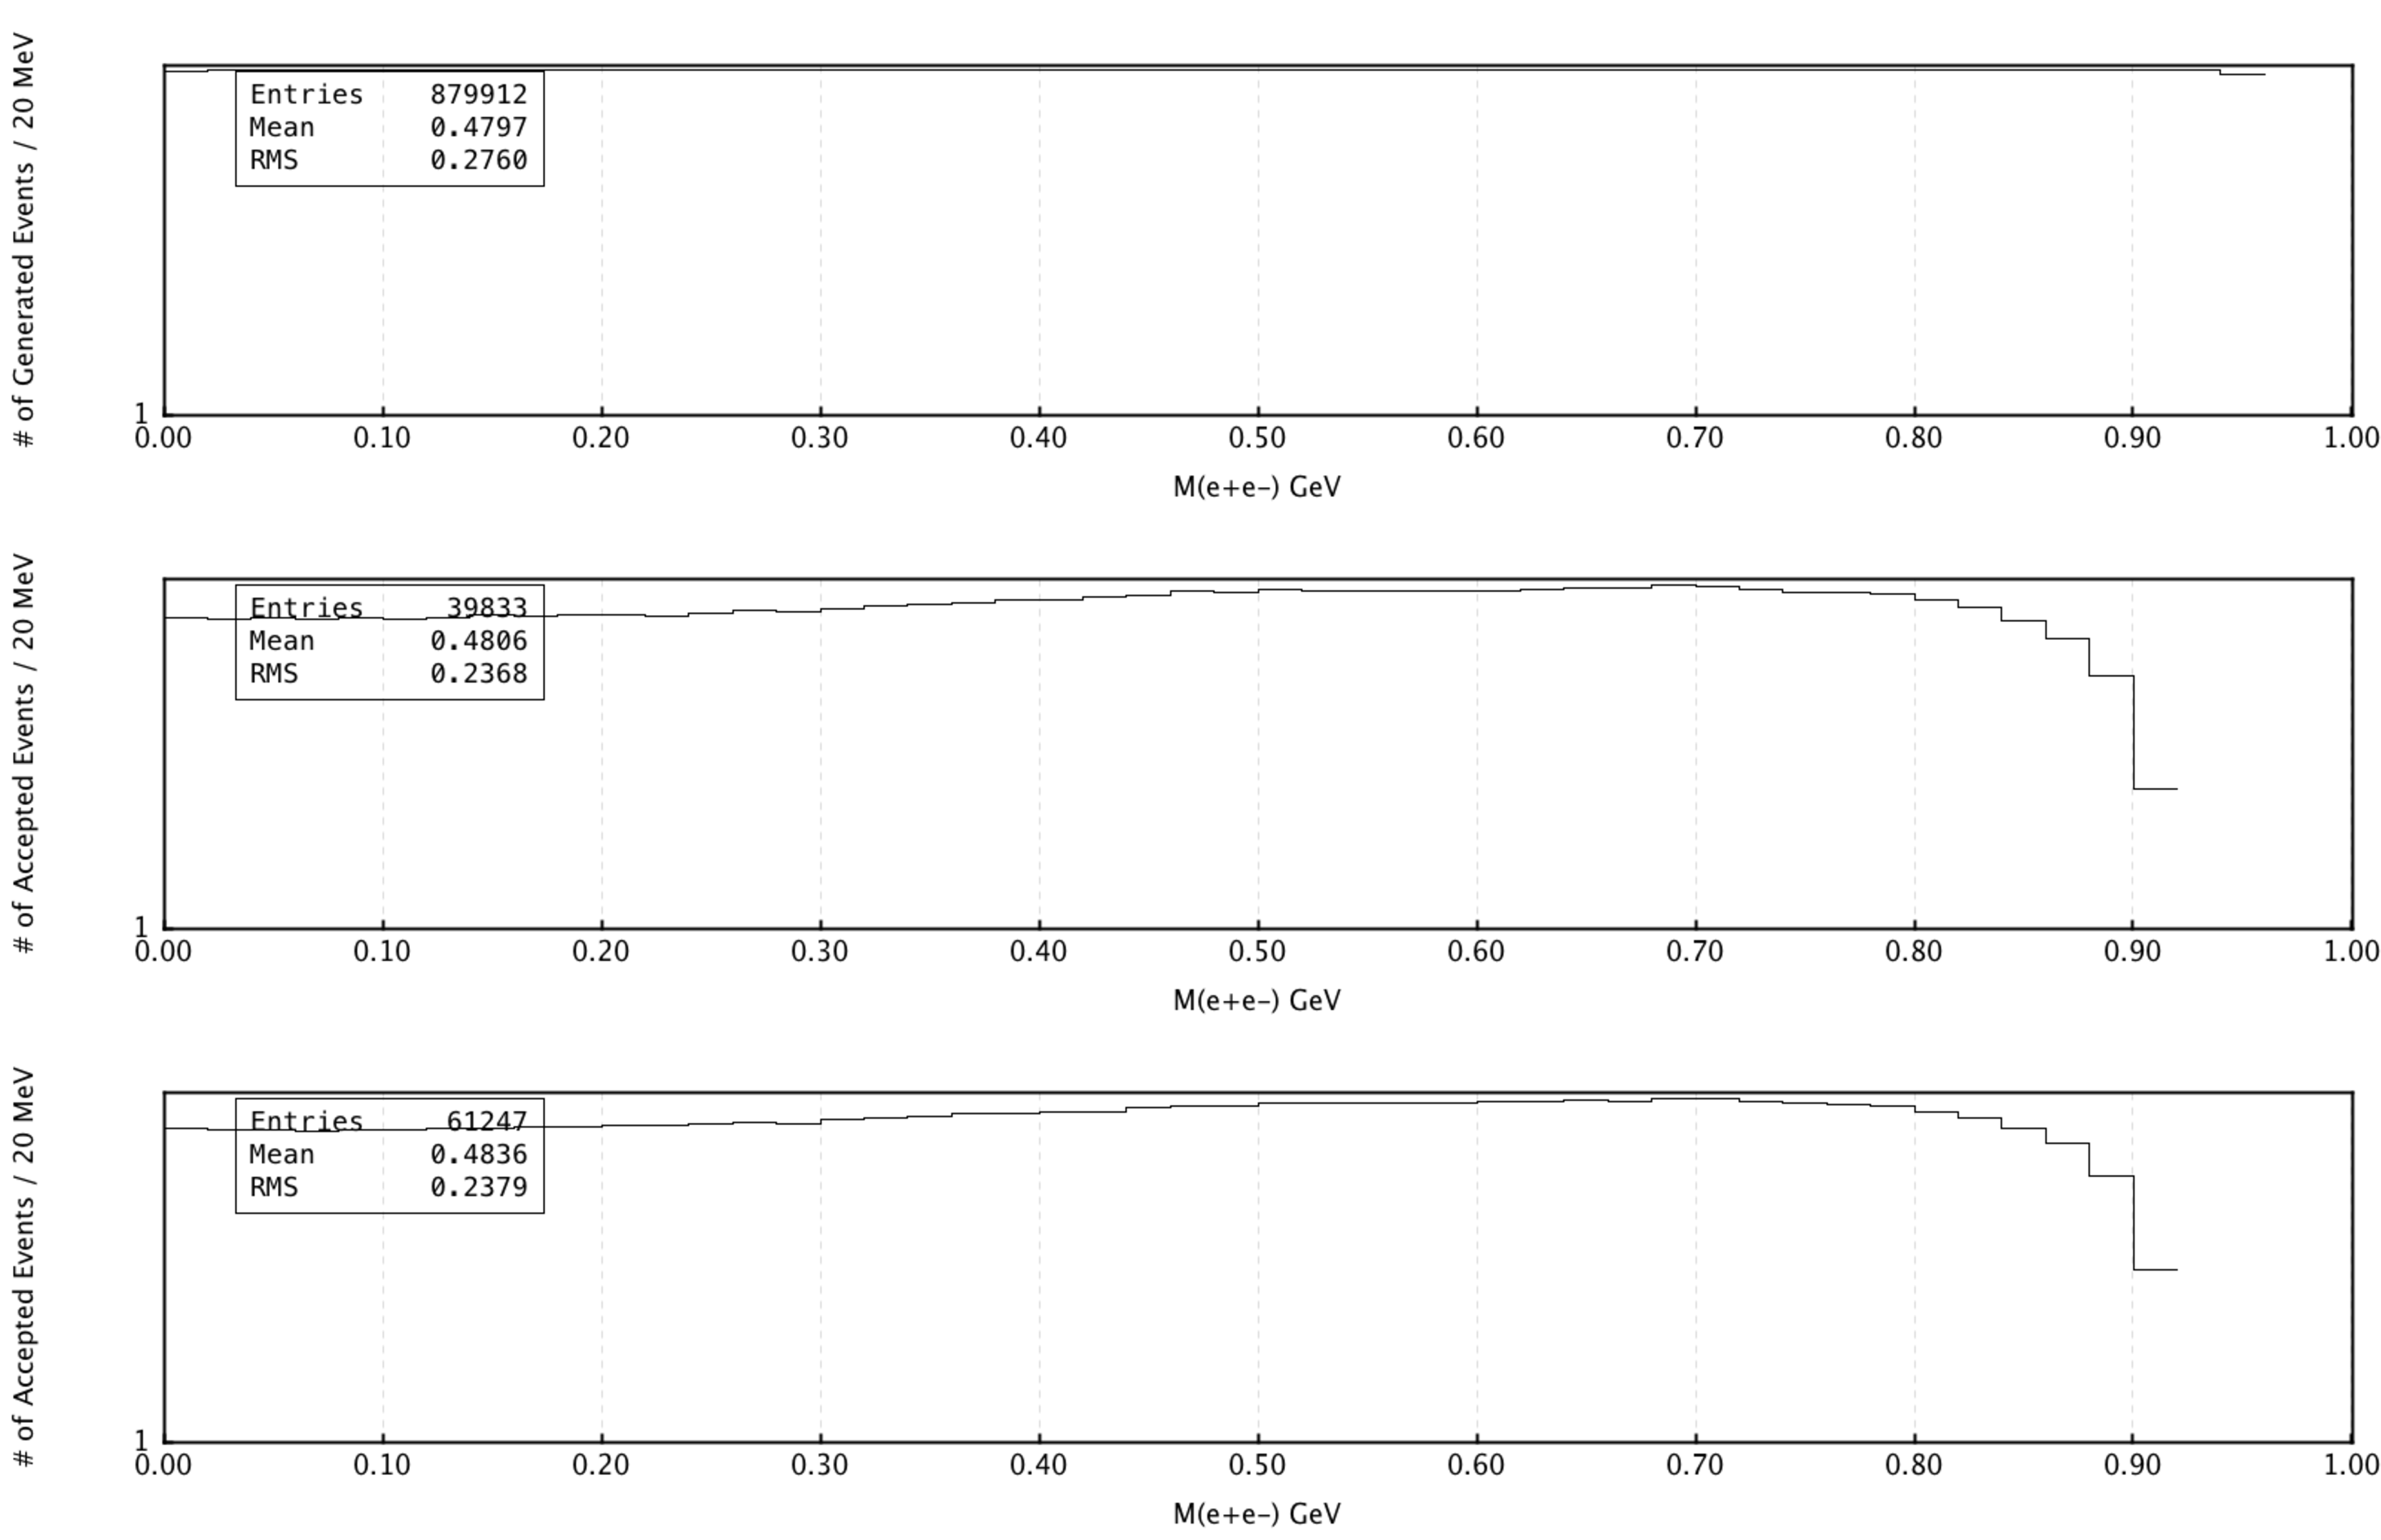
\includegraphics[width=\figwidth,height=2.6\qfigheight]{\grpath/counts/75_TORUS/FLAT/FLAT_Generated_Accepted.pdf}
%			\caption[Generated and Accepted counts, as a function of $M(\epem)$]{\label{fig:FLAT}{Generated events (Top), accepted events for an exclusive (Middle), inclusive(Bottom) reconstruction schemes as a function of $M(\epem)$. In all panels a Flat \epemT \ decay model was employed}}
%\end{center}\end{figure}
\FloatBarrier

\begin{figure}[h!]\begin{center}
		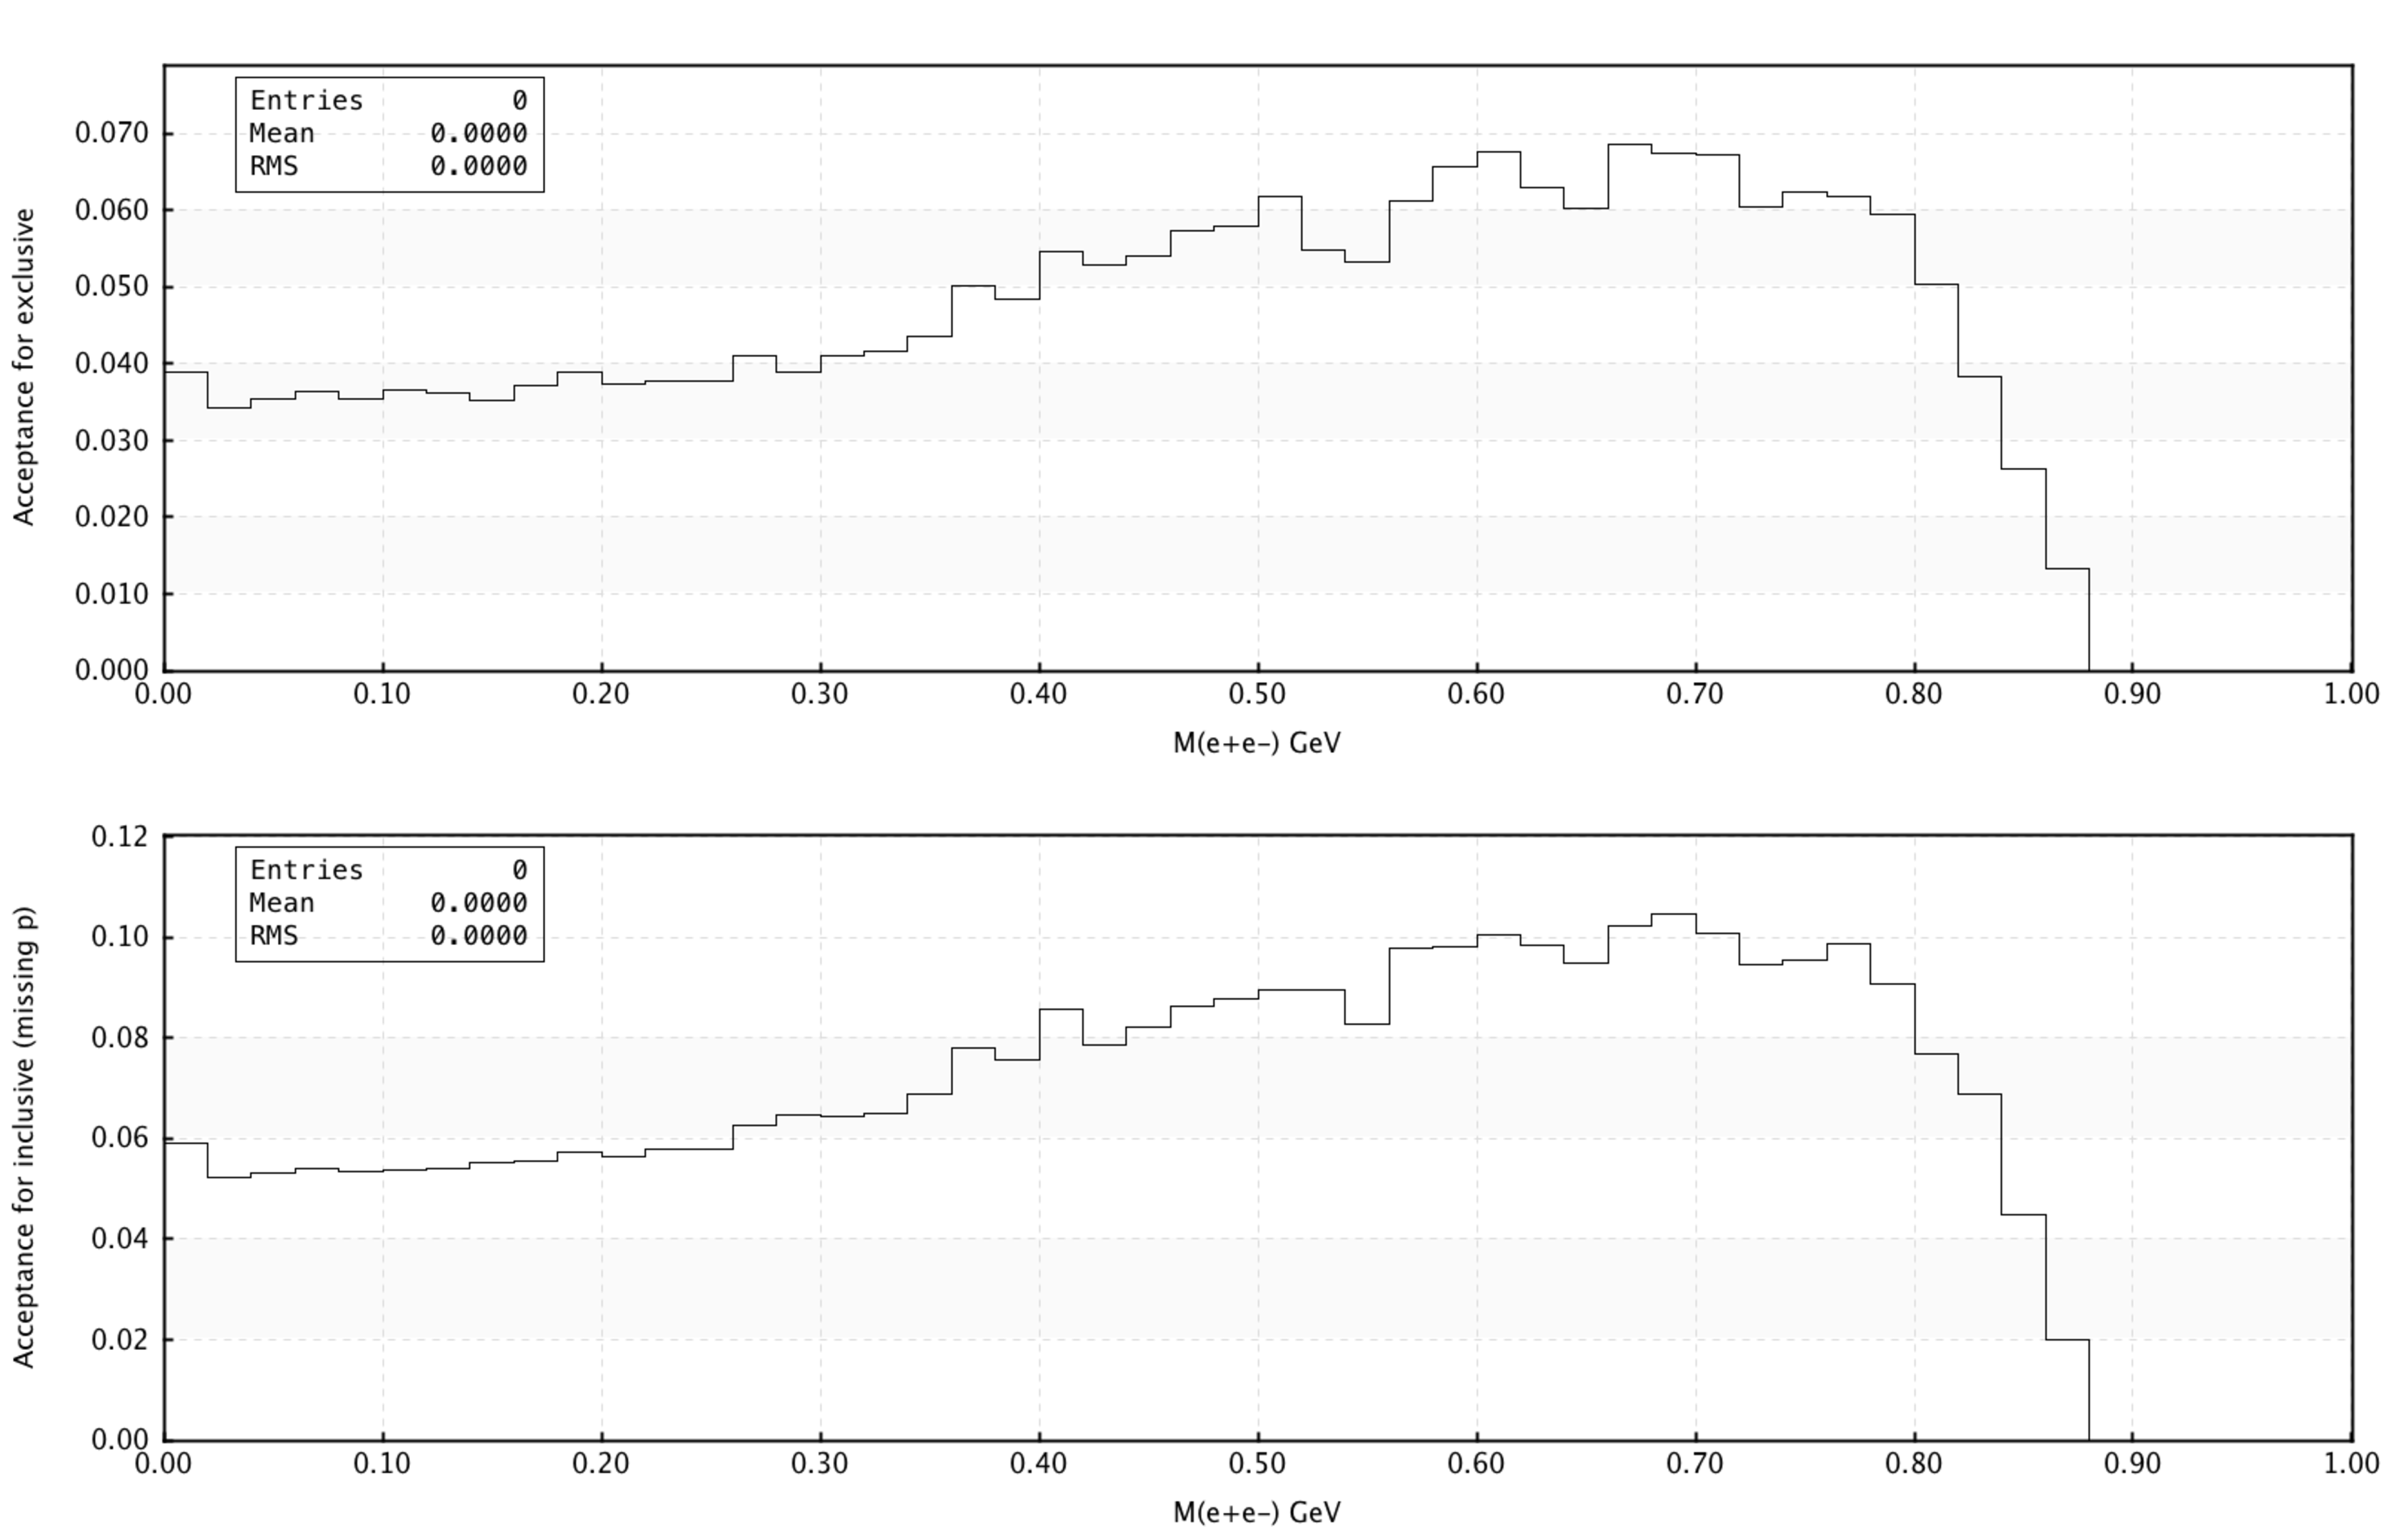
\includegraphics[width=\figwidth,height=1.2\qfigheight]{\grpath/counts/75_TORUS/VMD/VMD_Acceptance.pdf}
		\caption[Acceptance, as a function of $M(\epem)$]{\label{fig:VMDaccepted}{Acceptance using a VMD decay model, as a function of $M(\epem)$ for the exclusive (Top) and inclusive reconstruction scheme(Bottom). }}
\end{center}\end{figure}

 \begin{figure}[h!]\begin{center}
 		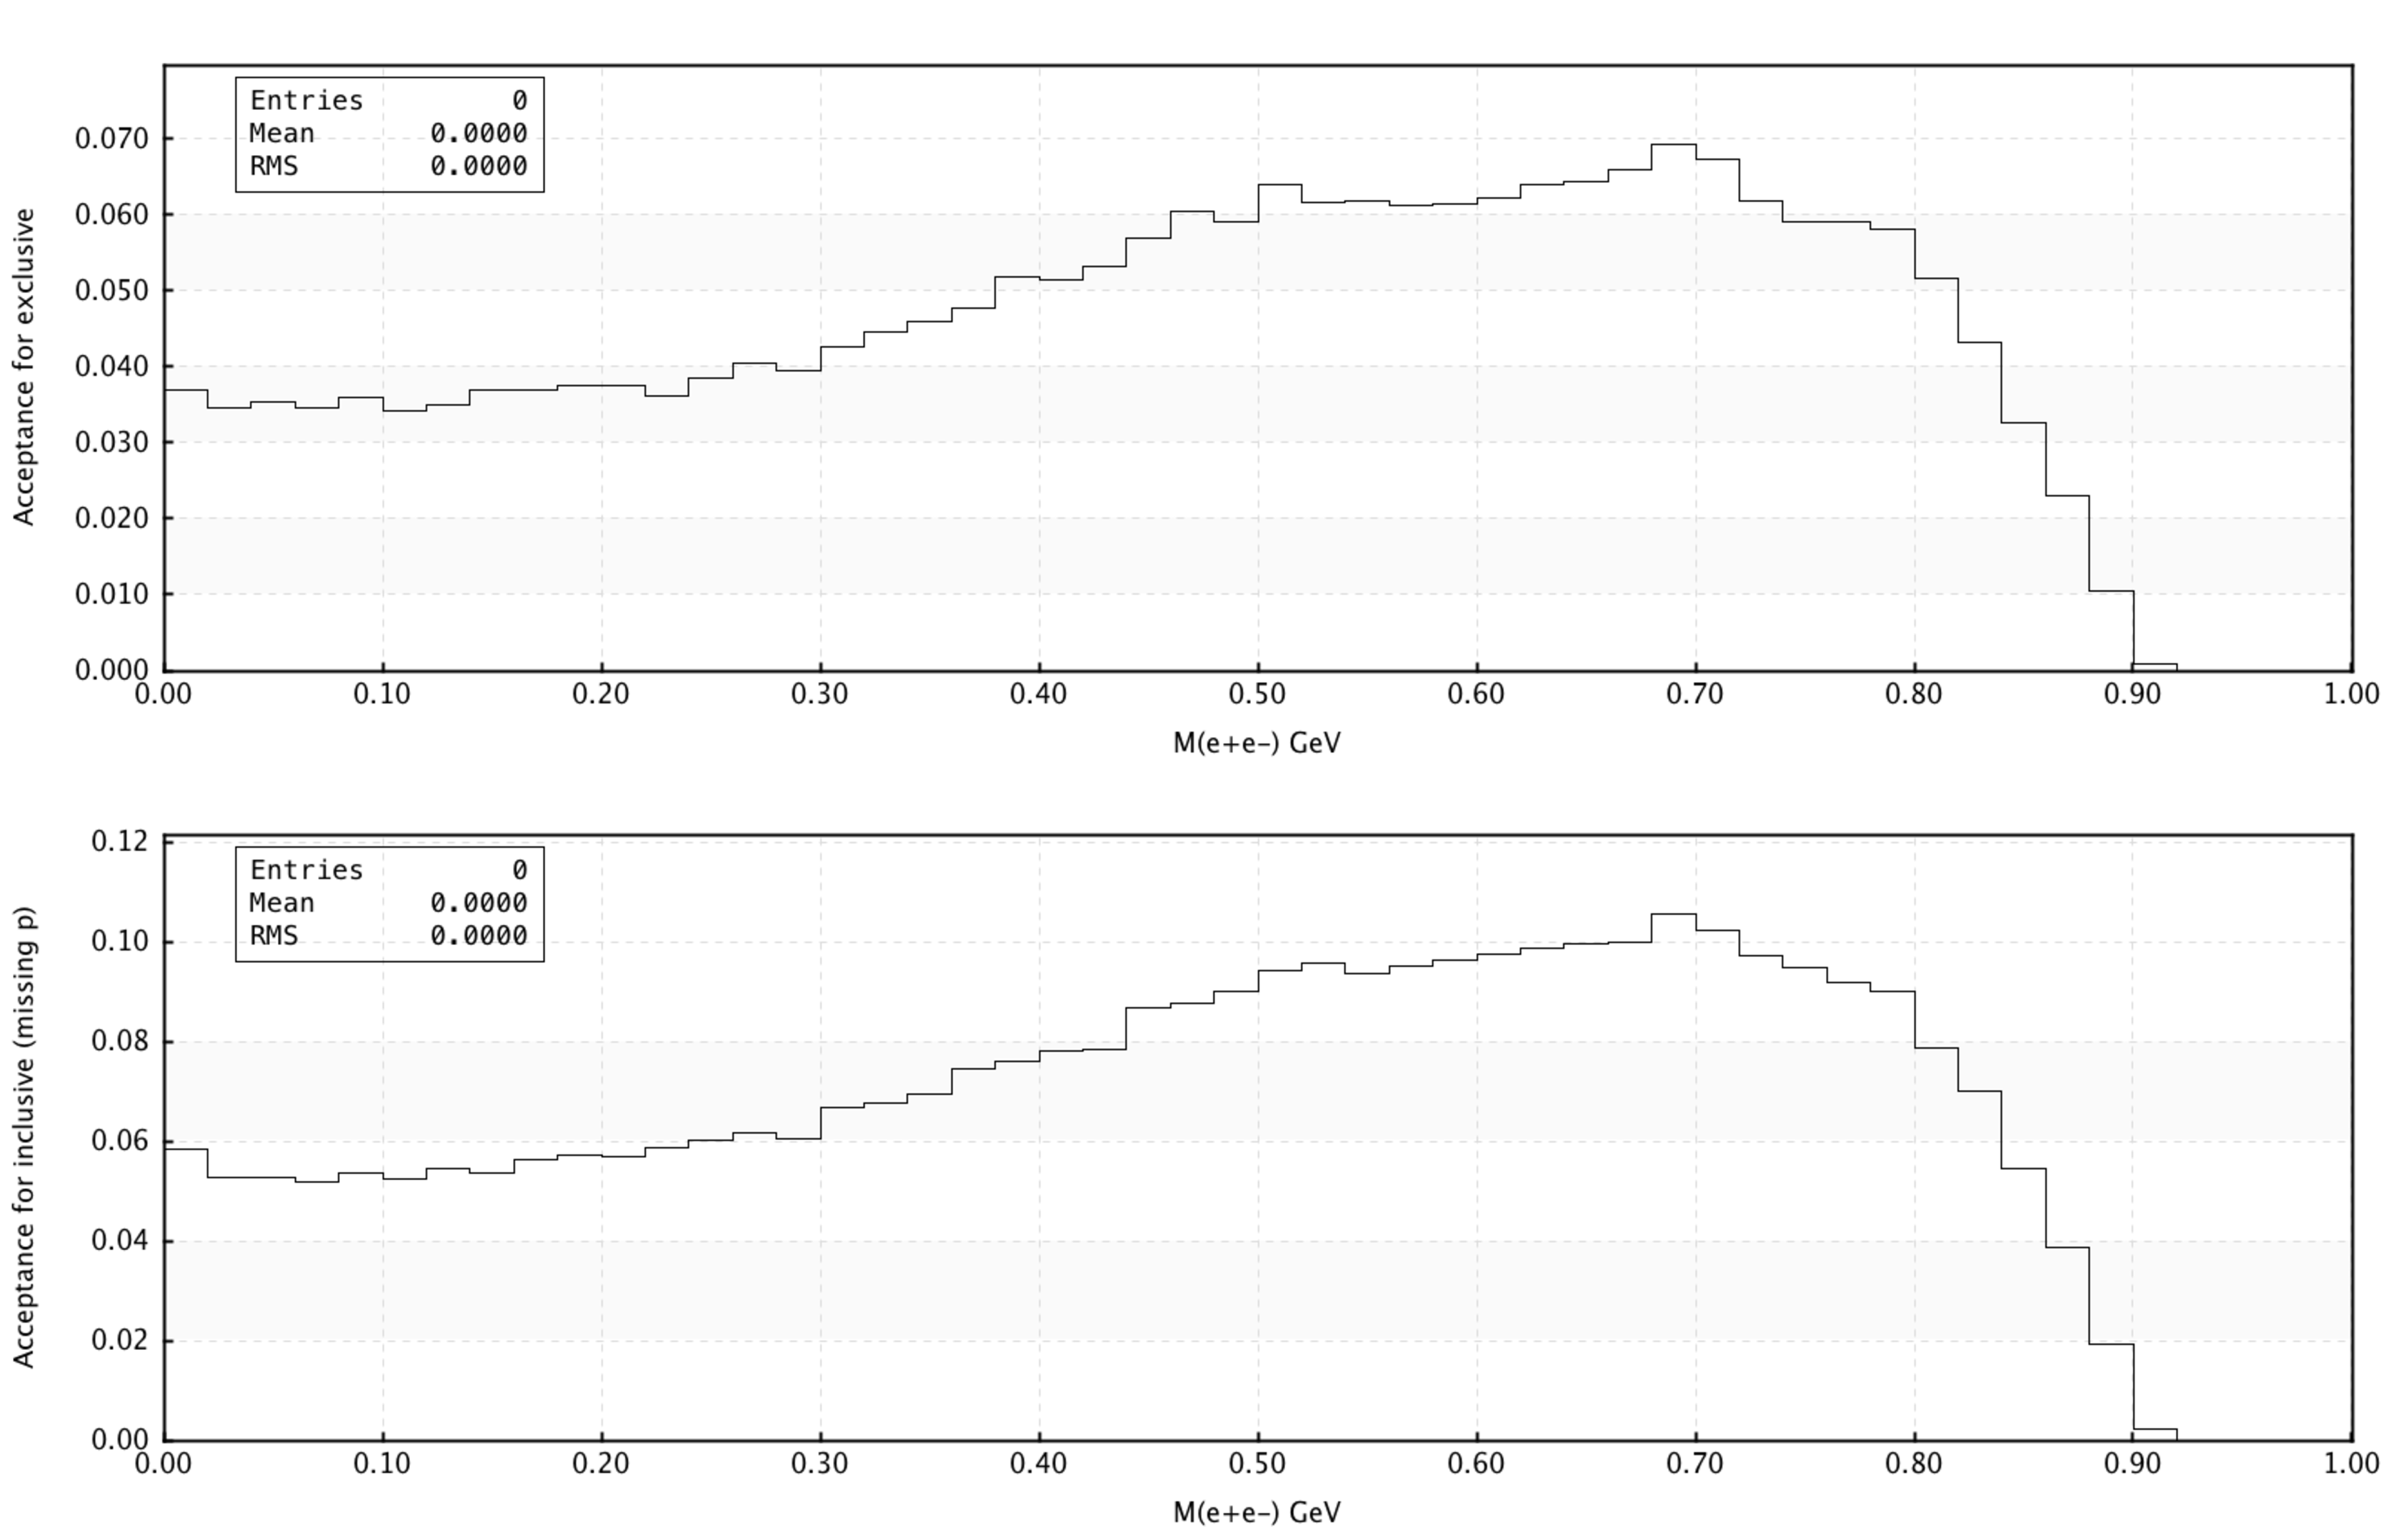
\includegraphics[width=\figwidth,height=1.2\qfigheight]{\grpath/counts/75_TORUS/FLAT/FLAT_Acceptance.pdf}
 		\caption[Acceptance, as a function of $M(\epem)$]{\label{fig:FLATaccepted}{Acceptance using a flat \epemT \ decay model, as a function of $M(\epem)$ for the exclusive (Top) and inclusive reconstruction scheme(Bottom).}}
 \end{center}\end{figure} 
\FloatBarrier




%%%%%%%%%%%%%%%%%%%%%%%%%%%%%%%%%%%%%%%
%THIS IS WHAT I ADDED:

\subsection{Calculating the Expected Yield}\label{sec:yield}
%\subsubsection{Calculating Photon Flux}\label{sec:calflux}
%A simple method for calculating the photon flux in CLAS12 is as follows; Using the fact that g12 had a photon flux of $7\cdot 10^7 \ \mathrm{\gamma/s}$ on a Au radiator of $10^{-4} \chi_0$ an expected $\sim 4\cdot 10^9  \mathrm{\gamma/s}$ will be seen in CLAS12 at ${\cal L} = 10^{35}\mathrm{cm^{-2}s^{-1}}$ on a 5~cm $\ell H_2$ target which is $\sim 5.7\cdot 10^{-3} \chi_0$. This number has been independently confirmed in a previous CLAS proposal~\cite{clas.proposal.meson}.

The expected yield for $ep\to e'p \etaP [\etaP\rightarrow p e^+e^- \gamma ]$ is calculated under the assumption, that the $\etaP$ electro-production cross-section can be deduced from the $\etaP$ photo-production cross-section. A qualitative justification of this assumption may be found in Fig.~\ref{fig:EtaProdX}. The shape of the cross-section distributions for $ep\rightarrow e'p\eta$, shown in the top row of Fig.~\ref{fig:EtaProdX}, are comparable to the corresponding distribution for $\gamma p\rightarrow p\eta$, plotted in the bottom row of Fig.~\ref{fig:EtaProdX}. The major difference is related to the scaling rule of $1/Q^2$, i.e. the electro-production cross-section might be approximated by the photo-production cross-section by scaling down the latter one by $1/Q^2$.

\begin{figure}[htbp]\begin{center}
		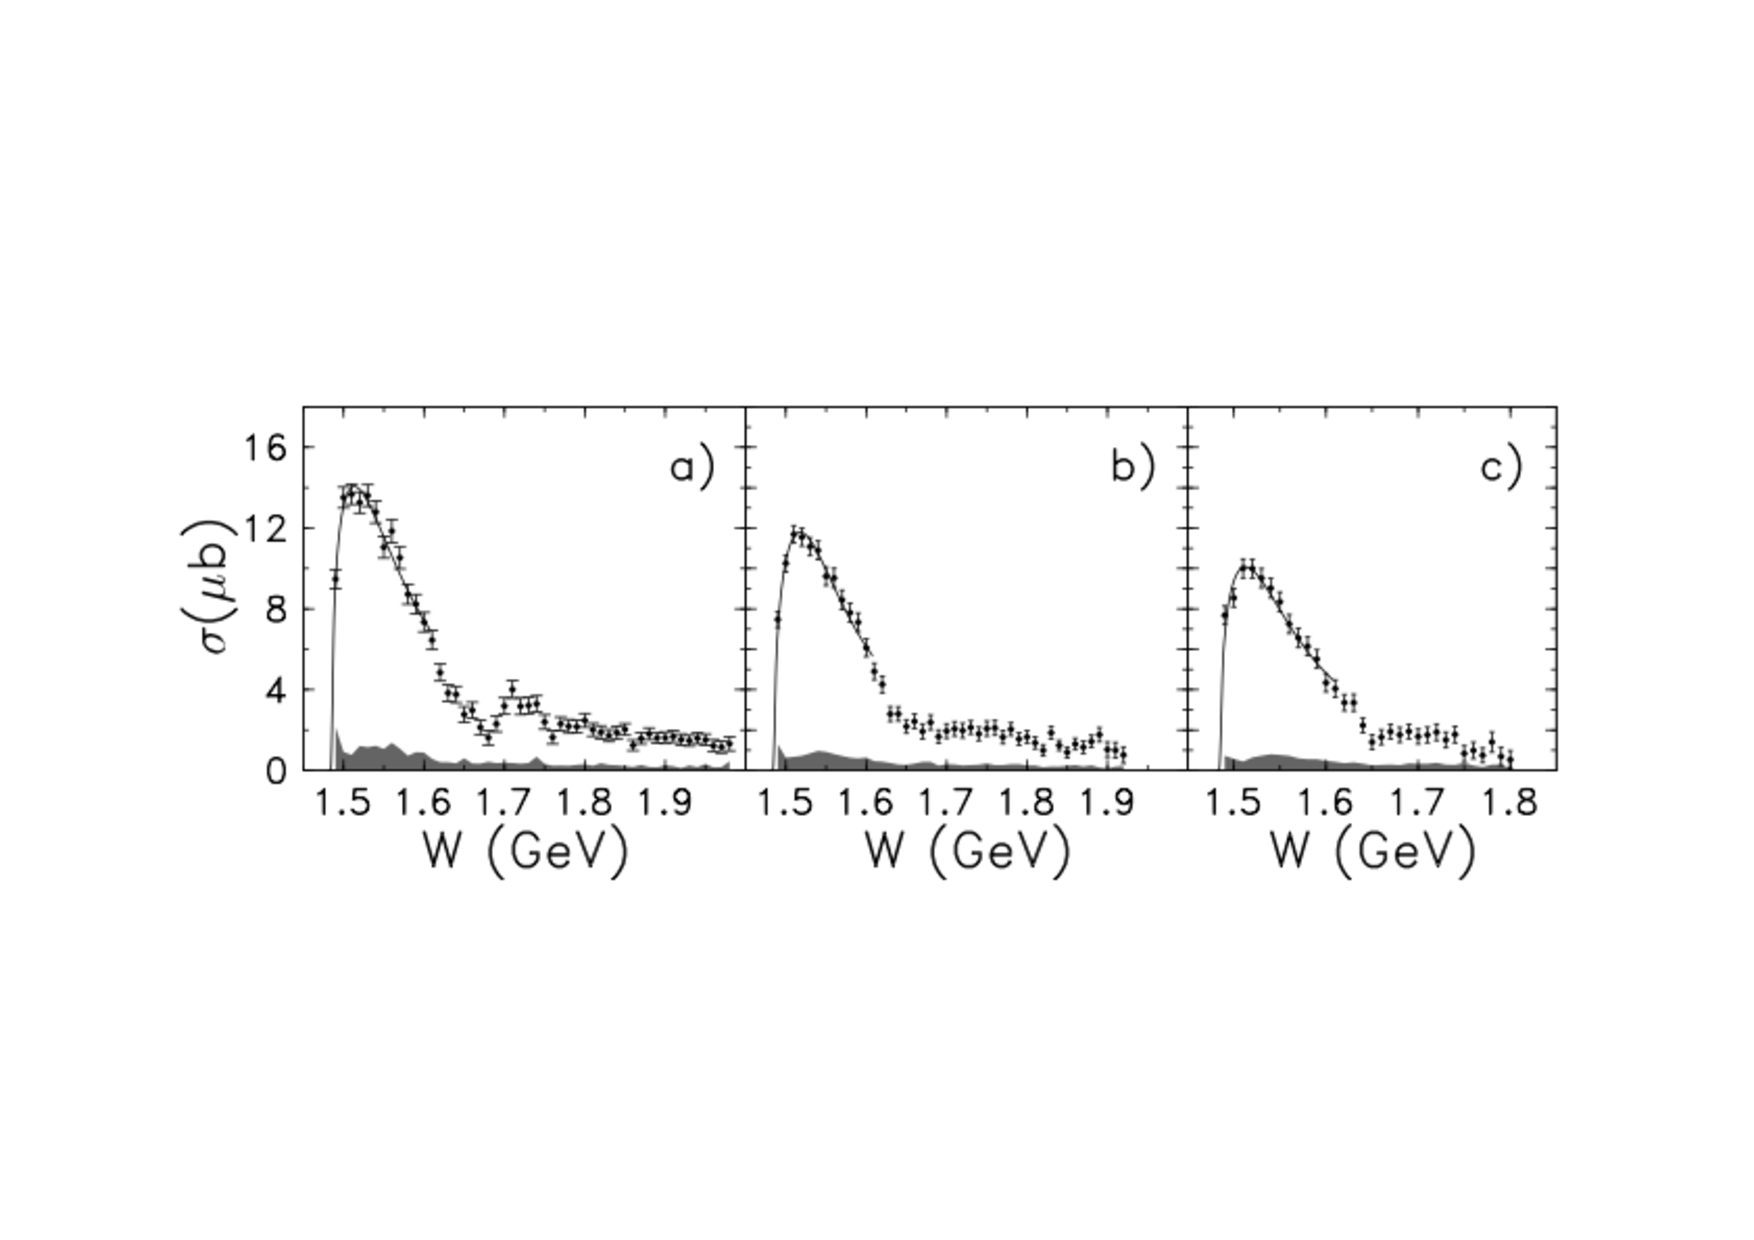
\includegraphics[width=\figwidth,height=1.2\qfigheight]{\grpath/XSection/eta_phot_electXSection.pdf}\\
		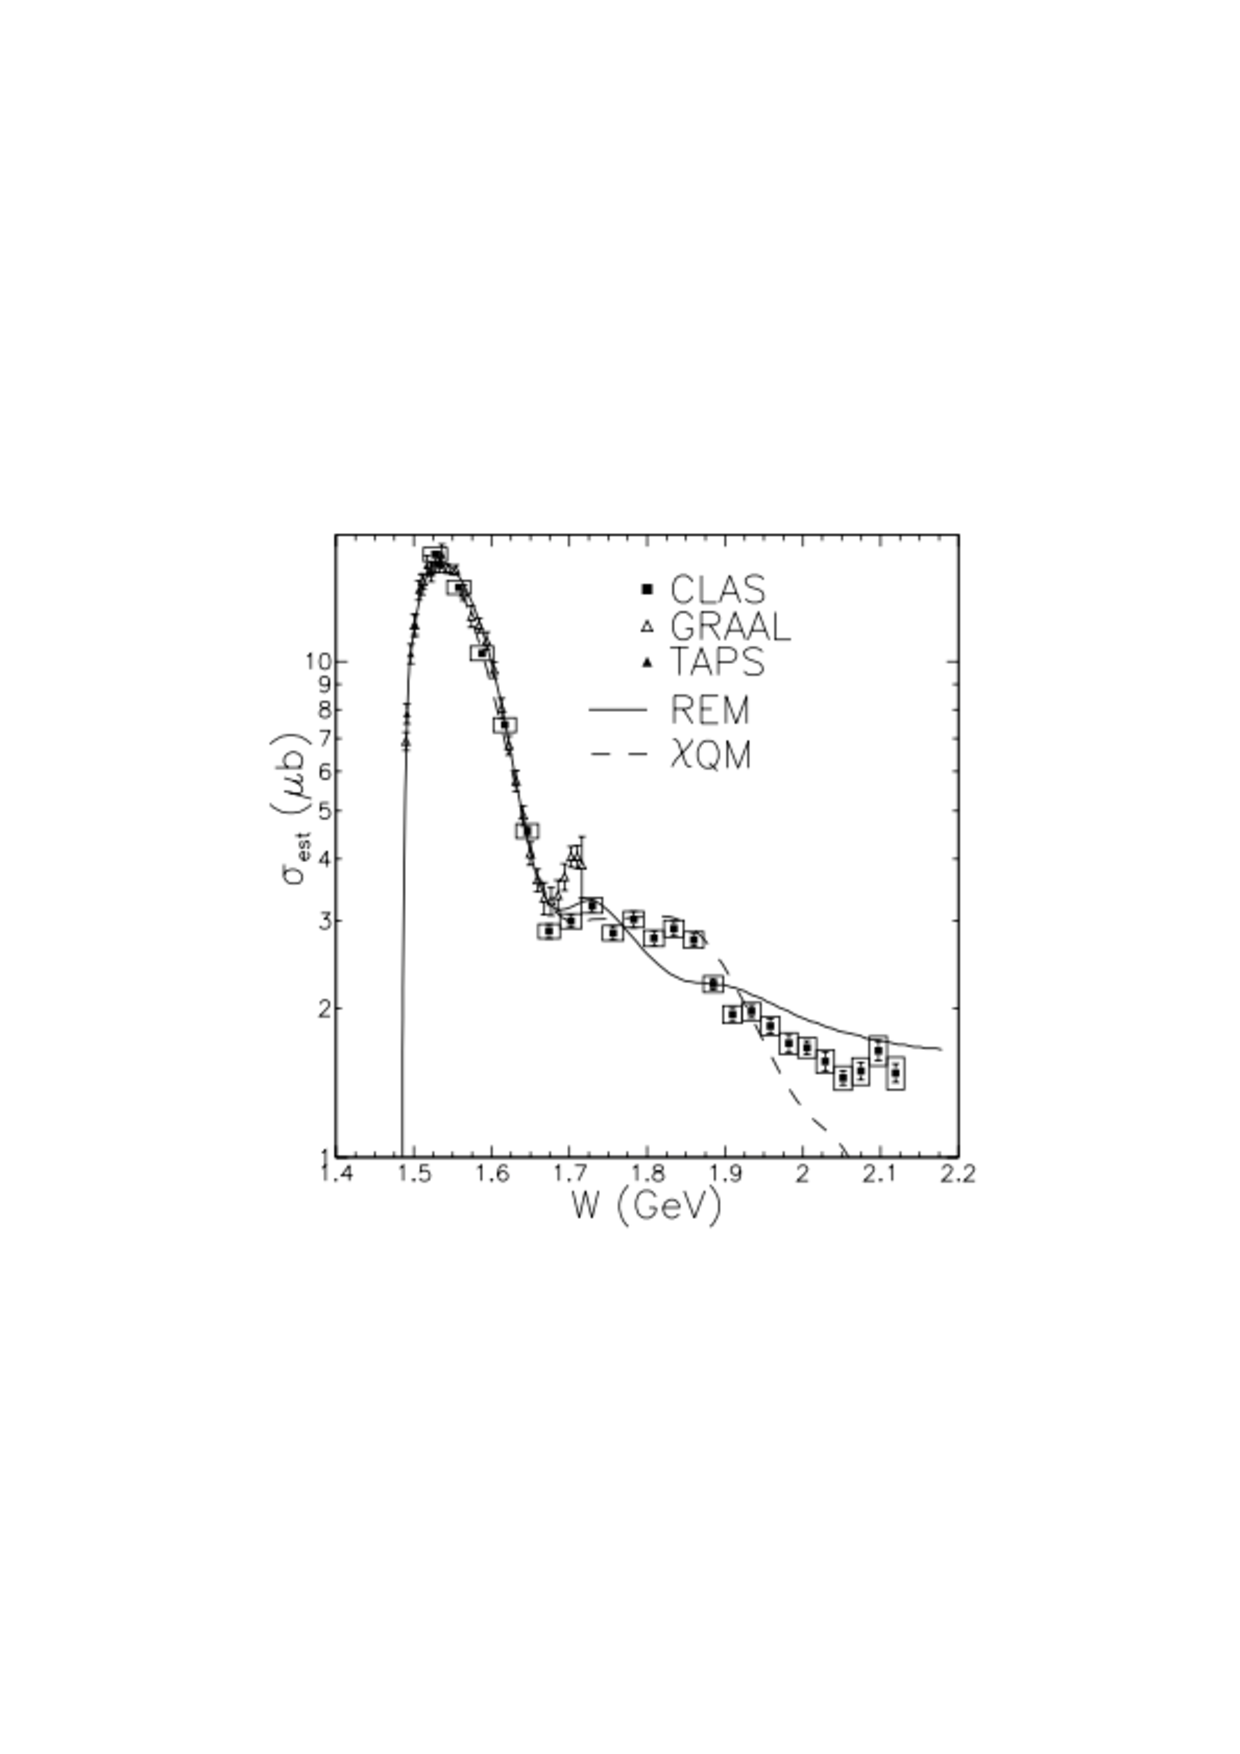
\includegraphics[width=0.7\figwidth,height=0.9\qfigheight]{\grpath/XSection/eta_phot_prodXSection.pdf}
		\caption[eta el-prod. XSection]{\label{fig:EtaProdX}{Integrated cross-section for $ep\to e'p\eta$ (Top) for: (a) $Q^2=0.625(GeV/c)^2$, (b) $Q^2=0.875(GeV/c)^2$, (a) $Q^2=1.125(GeV/c)^2$~\cite{etaelect} and for $\gamma p\rightarrow p\eta$ (Bottom)~\cite{etaphoto}.}}
\end{center}\end{figure}

\FloatBarrier

The top row of Fig.~\ref{fig:EtaPProdX} shows the total photo-production cross-section for hadrons in comparison with the photo-production cross-section for $\etaP$ (see bottom row of Fig.~\ref{fig:EtaPProdX}). Due to the considerations made above, these two cross-section distributions might be directly translated to the corresponding electro-production cross-sections. Using the distributions shown in Fig.~\ref{fig:EtaPProdX}, one might define the following ratio $R(W)$:

\begin{equation}
 R(W) = \frac{\sigma(W)}{\etaP\text{ integrated } \sigma(W)}
\label{XsecR}
\end{equation}

\begin{figure}[h!]\begin{center}
		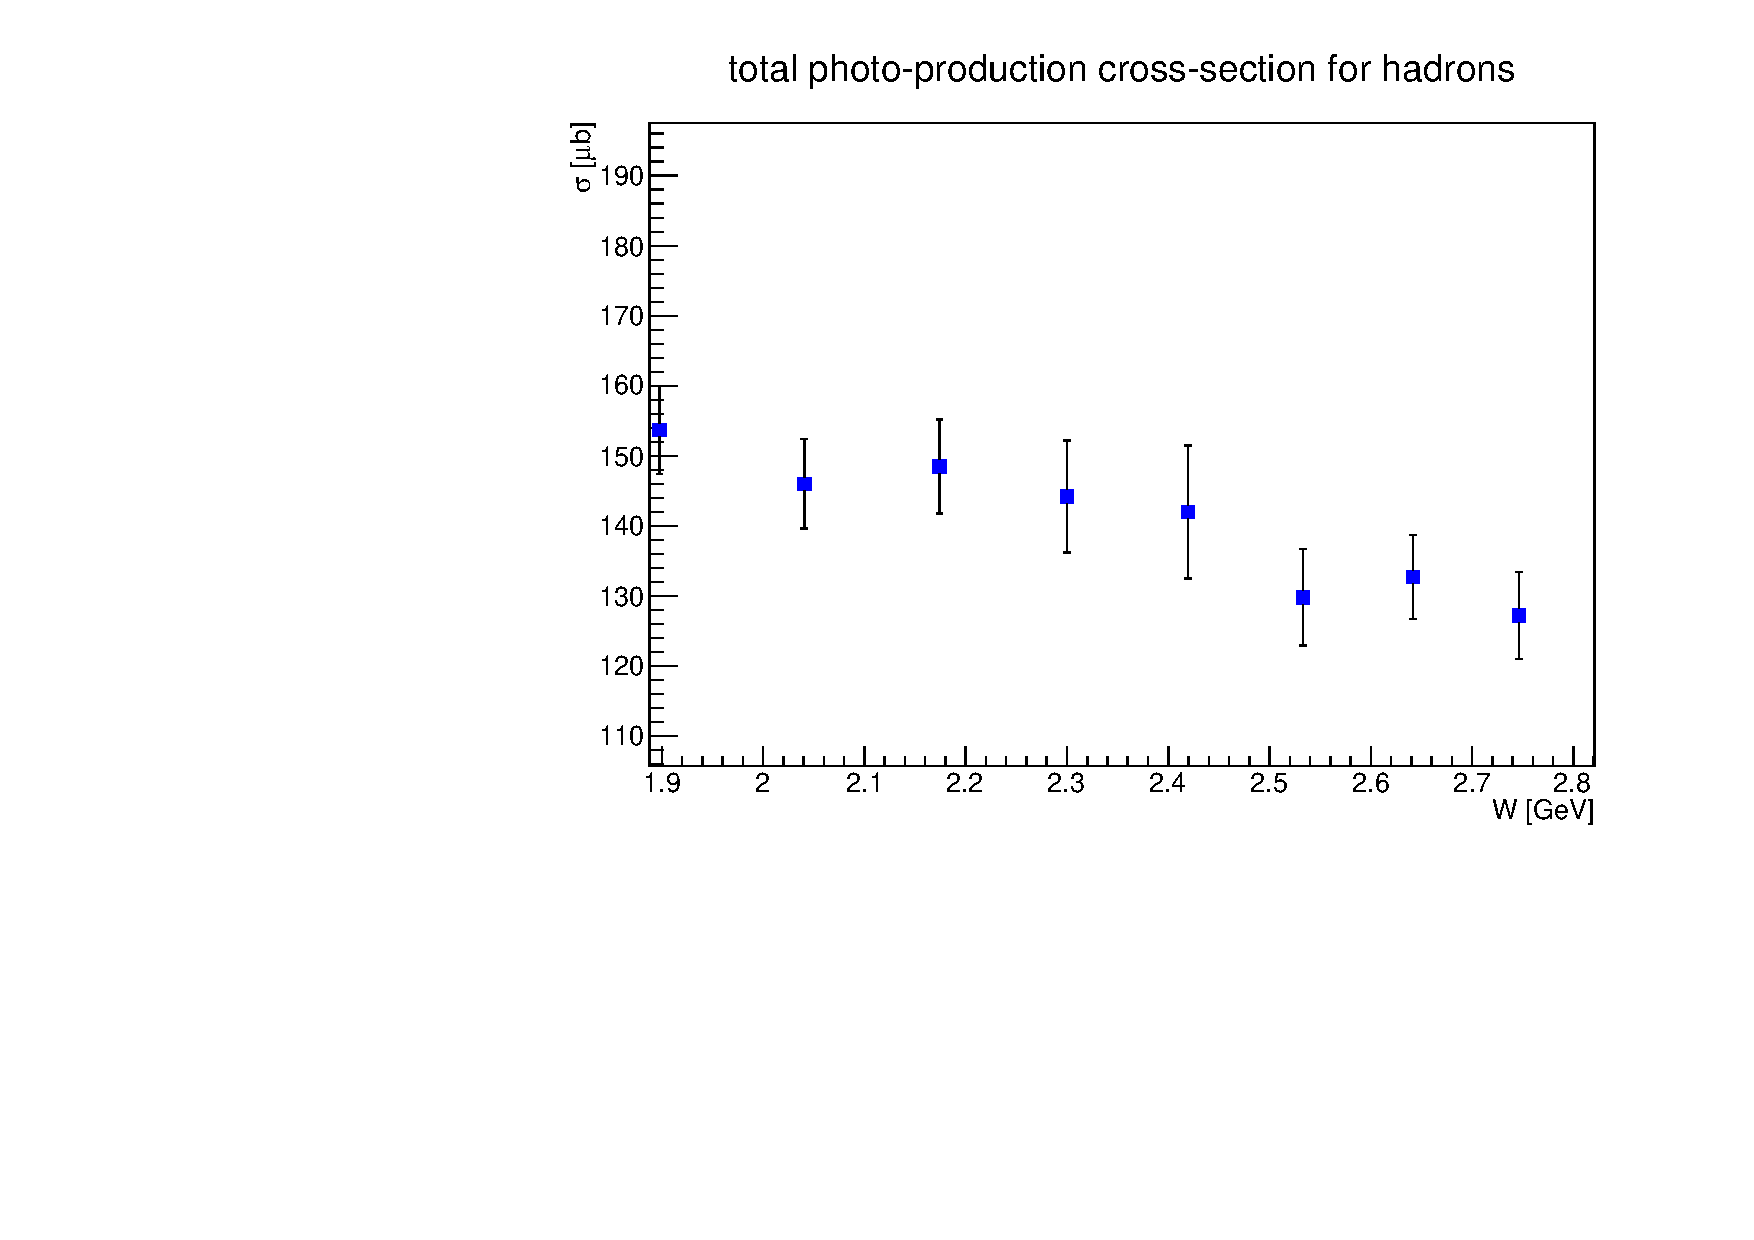
\includegraphics[width=0.9\figwidth,height=0.9\qfigheight]{\grpath/XSection/hadron_prod_photoproduction.pdf}\\
		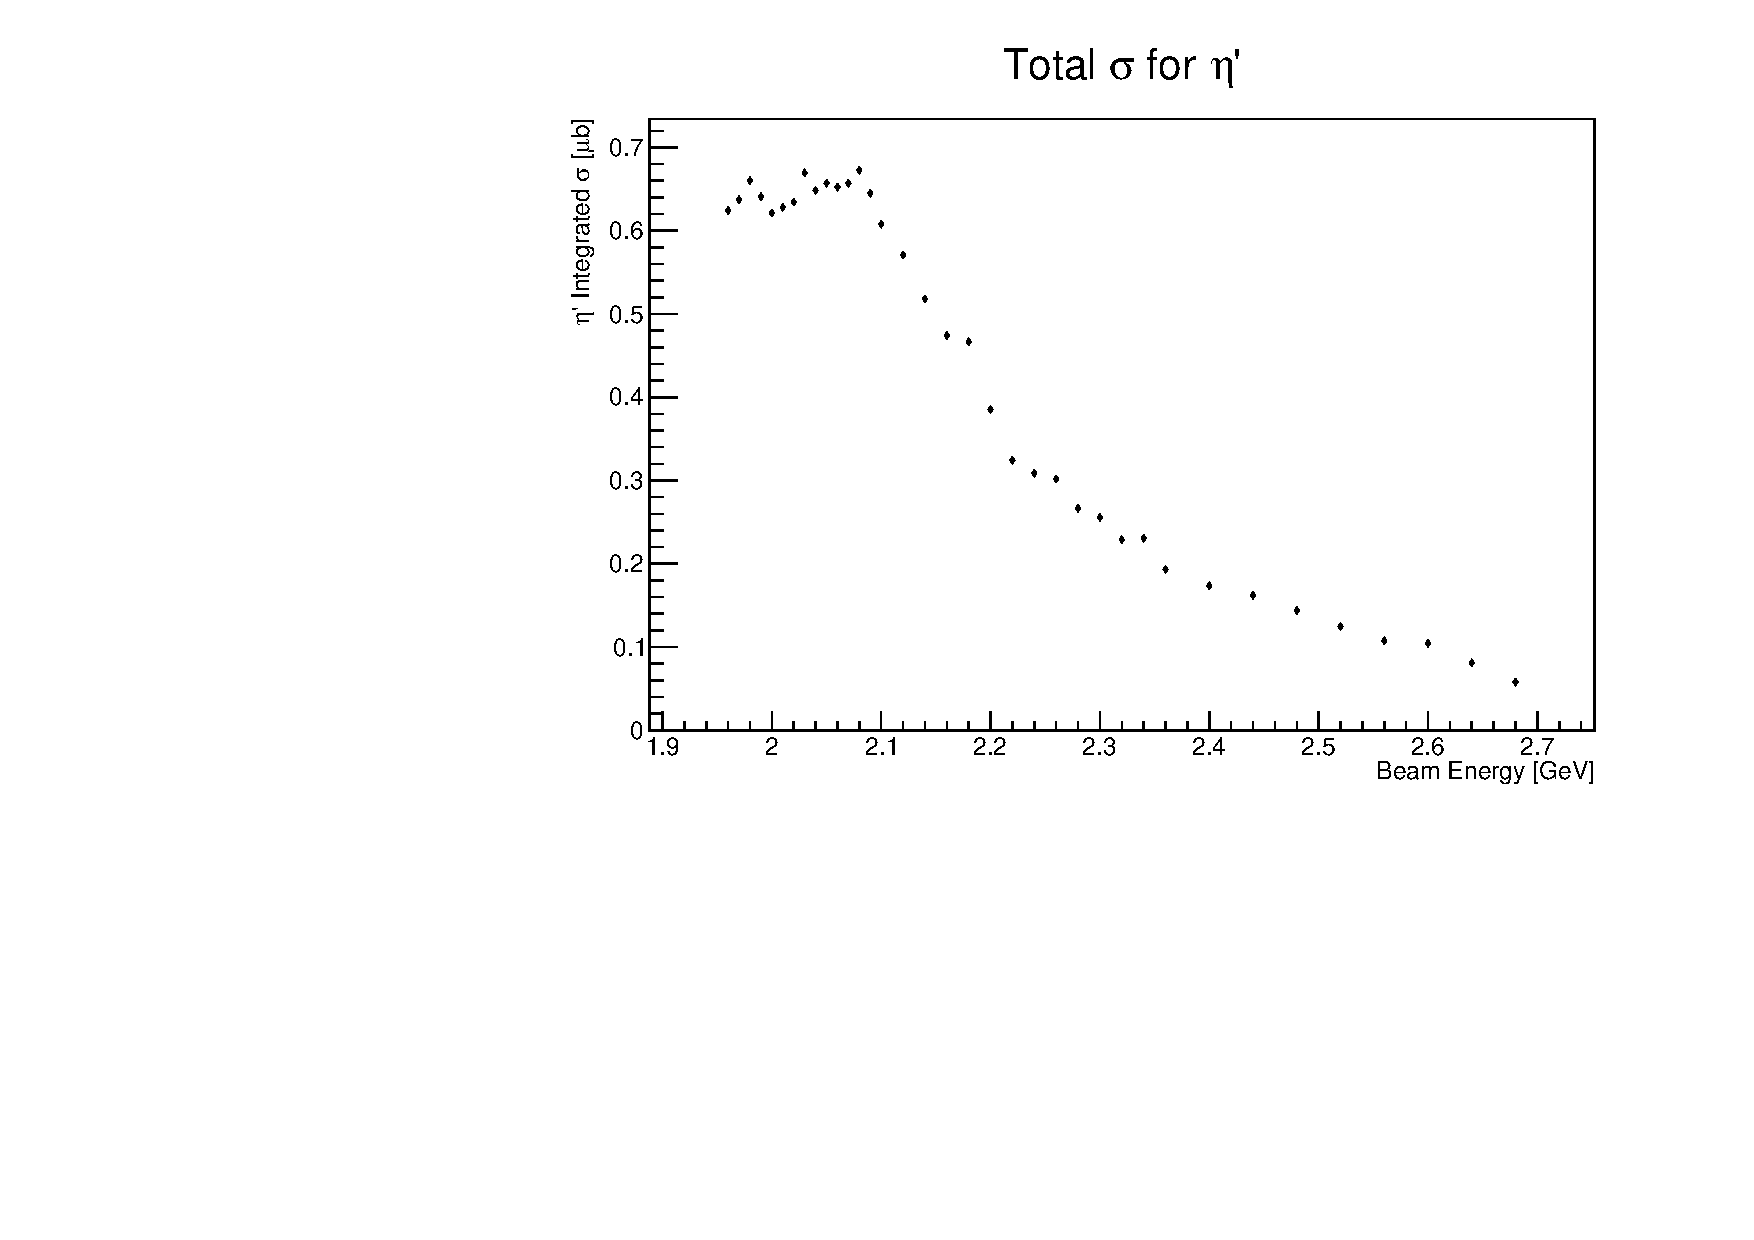
\includegraphics[width=0.9\figwidth,height=0.9\qfigheight]{\grpath/XSection/etaP_total_XSection.pdf}
		\caption[etaP phot-prod. XSection]{\label{fig:EtaPProdX}{Integrated cross-section for $\gamma p\rightarrow pX$ (Top) and $\gamma p\rightarrow p\etaP$ (Bottom) as a function of $W$.}}
\end{center}\end{figure}

The rate for mesons in electro-production where the scattered electron is left undetected is $\sim 140\,\rm{kHz}$~\cite{Sargsyan}. This rate needs to be scaled down by $R(W)$ in order to achieve the corresponding rate for $\etaP$ production. This leads to:

\begin{equation}
 \etaP\text{ total rates / 80 Days }(W) = 140\,\rm{kHz}\cdot \frac{86,400\mathrm{\ seconds}}{\text{80 days}}\cdot \frac{1}{R(W)}
\label{etaPRate}
\end{equation}

A plot of Eq.~\ref{etaPRate} is shown in Fig.~\ref{fig:EtaPRate} (left y-axis). The total $\etaP\rightarrow\epem\gamma$ rates per 80 days, and as a function $W$, is calculated by multiplying Eq.\ref{etaPRate} with the product of the average detection efficiency $\epsilon\approx 5\%$ as well as the branching fraction $\mathcal{BR} $ for $\etaP\rightarrow\epem\gamma$. The corresponding plot is shown in Fig.~\ref{fig:EtaPRate} (right y-axis). Obviously, the total number $N_{tot}$ of expected $\etaP\rightarrow\epem\gamma$ events after 80 days of measurement is given by the integral of Fig.~\ref{fig:EtaPRate} over $W$. This leads to the expected yield:

\begin{equation}
  N_{tot} = \int\limits_{1.9\,\rm{GeV}}^{2.8\,\rm{GeV}} \Big[ {\color{red}{N(W)_{\etaP\rightarrow\epem\gamma\text{ / 80 Days }}}} \Big]dW = \mathrm{\frac{52,100 \ events}{80 Days}}
\label{yield}
\end{equation}


\begin{figure}[h!]\begin{center}
		\includegraphics[width=0.9\figwidth,height=0.9\qfigheight]{\grpath/XSection/Total_rates.pdf}\\
		\caption[etaP rates]{\label{fig:EtaPRate}{Total $\etaP$ production rate per 80 days (left y-axis) and total $\etaP\rightarrow \epem\gamma$ rates per 80 days (right y-axis) as a function of $W$. Both rates have been calculated according to Eq.~\ref{etaPRate}}}
\end{center}\end{figure}


%%%%%%%%%%%%%%%%%%%%%%%%%%%%%%%%%%%%%%%





%\subsubsection{Expected Results}
%To extrapolate the number of $\etaP$ \ produced in 
%\\
%The average number of $\mathrm{meson} \to \epem X$ expected in CLAS12 can be calculated as:
%\begin{align}
%\bar{N}(\epem)_{\mathrm{meson}  \to \epem X} = \Phi \epsilon(\epem)\bar{\sigma} \rho_{\ell_{H_2}}\ell_{target}N_A \frac{\Gamma_{\mathrm{tot}_\mathrm{meson} }}{\Gamma_{\mathrm{meson}  \to \epem X}}\ ,
%\end{align}
%where $\Phi$ is the photon flux estimated in Sec.~\ref{sec:calflux}, $\epsilon$ is the acceptance, $\bar{\sigma}$ is the total cross-section, $\rho_{\ell_{H_2}}$ is the atomic density of $\ell_{H_2}$, $\ell_{target}$ is the target length, $N_A$ is Avogadro's constant, and $\frac{\Gamma_{\mathrm{tot}_\mathrm{meson}}}{\Gamma_{\mathrm{meson} \to \epem X}}$ is the total branching fraction of the meson decaying into $\epem X$.
%Using the lepton acceptance shown is Sec.~\ref{sec.reconstruction} the average number of \etaTP \  per $M(\epem)$ can be seen in Fig.~\ref{fig:etayield}.
% \begin{figure}[h!]\begin{center}
% \subfloat[$\etaP$ Dalitz and conversion spectra][]{ %Feynman diagram of $\etaP$ two photon decay
%	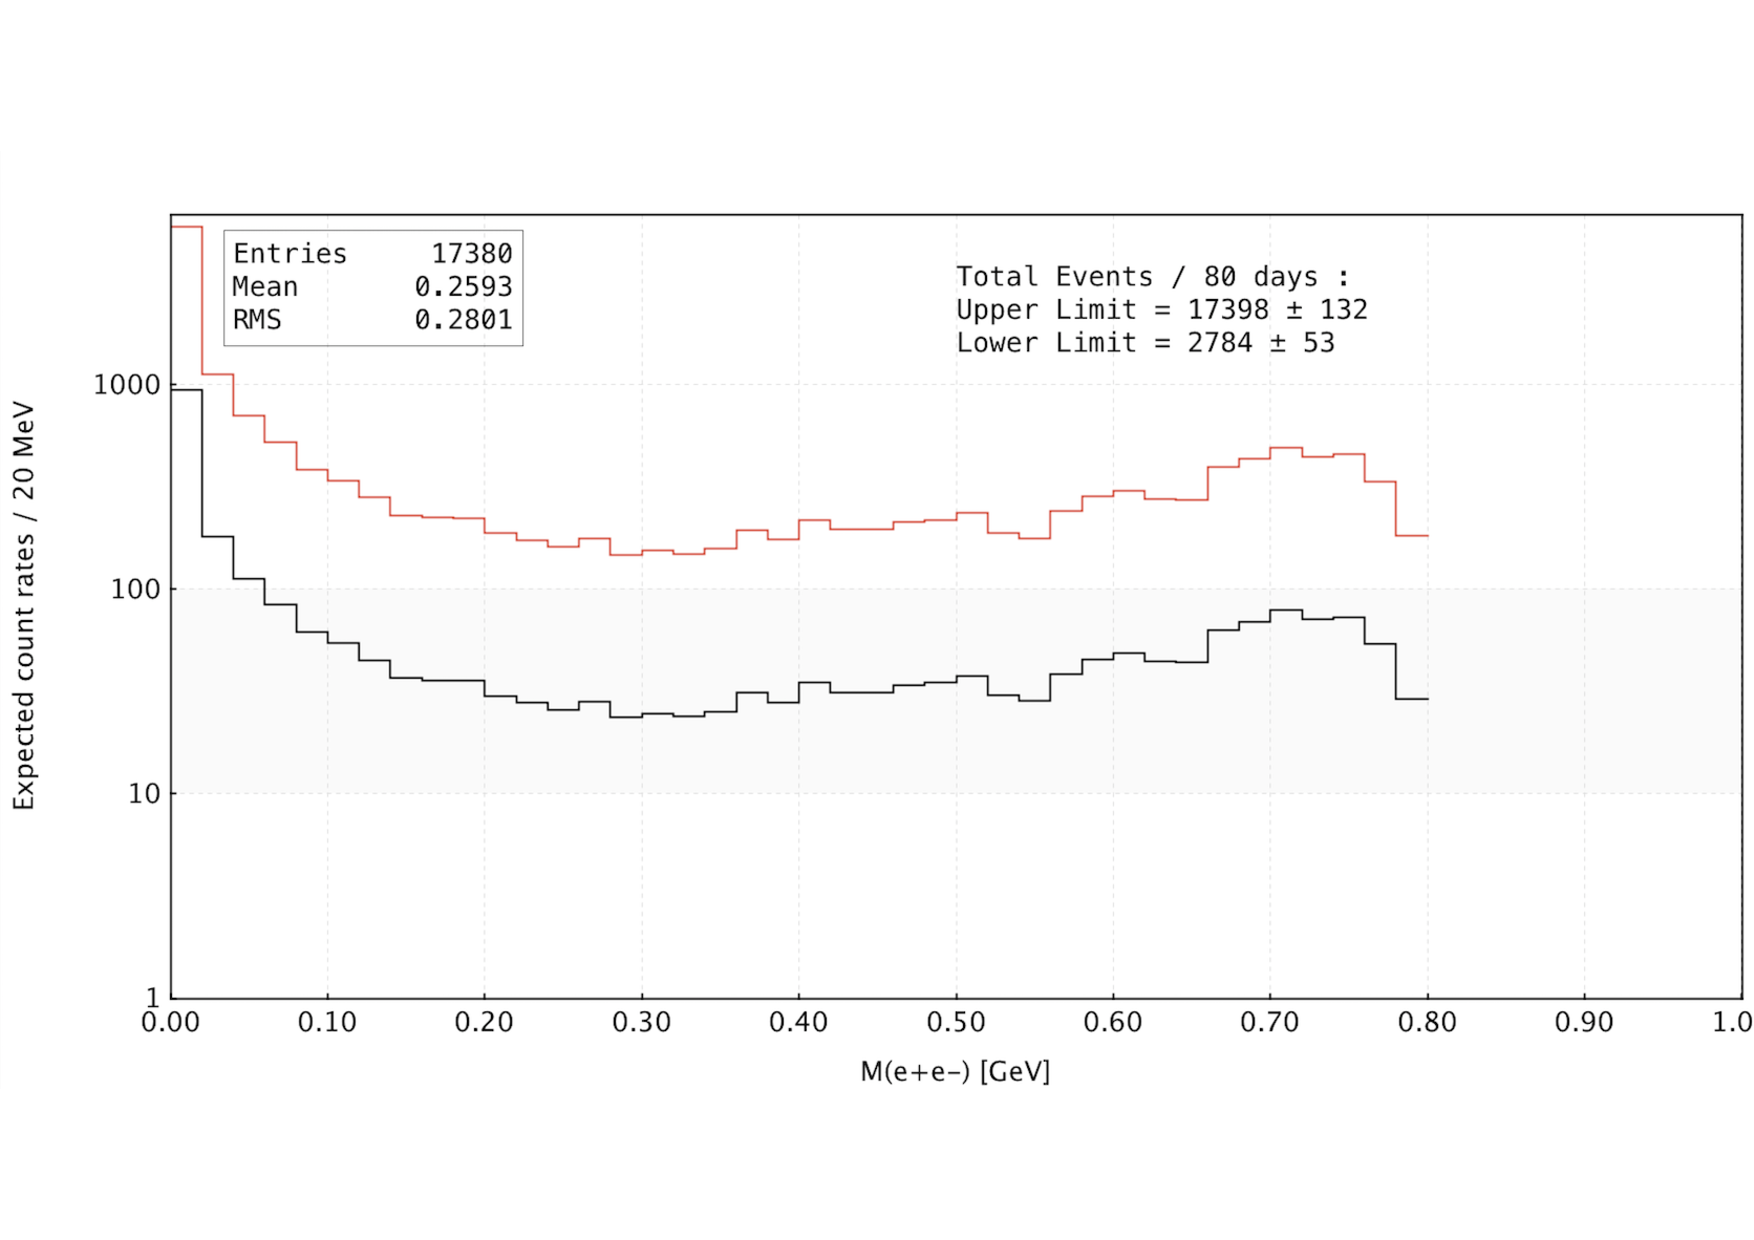
\includegraphics[width=0.8\columnwidth,height=1.0\qfigheight]{\grpath/counts/75_TORUS/VMD/VMD_Excluvise_count_rate.pdf}\label{fig:etap_count_exclu}
%	}
%\\
%\subfloat[$\phi$ Dalitz and conversion spectra][]{ %Feynman diagram of $\etaP$ Dalitz decay
%	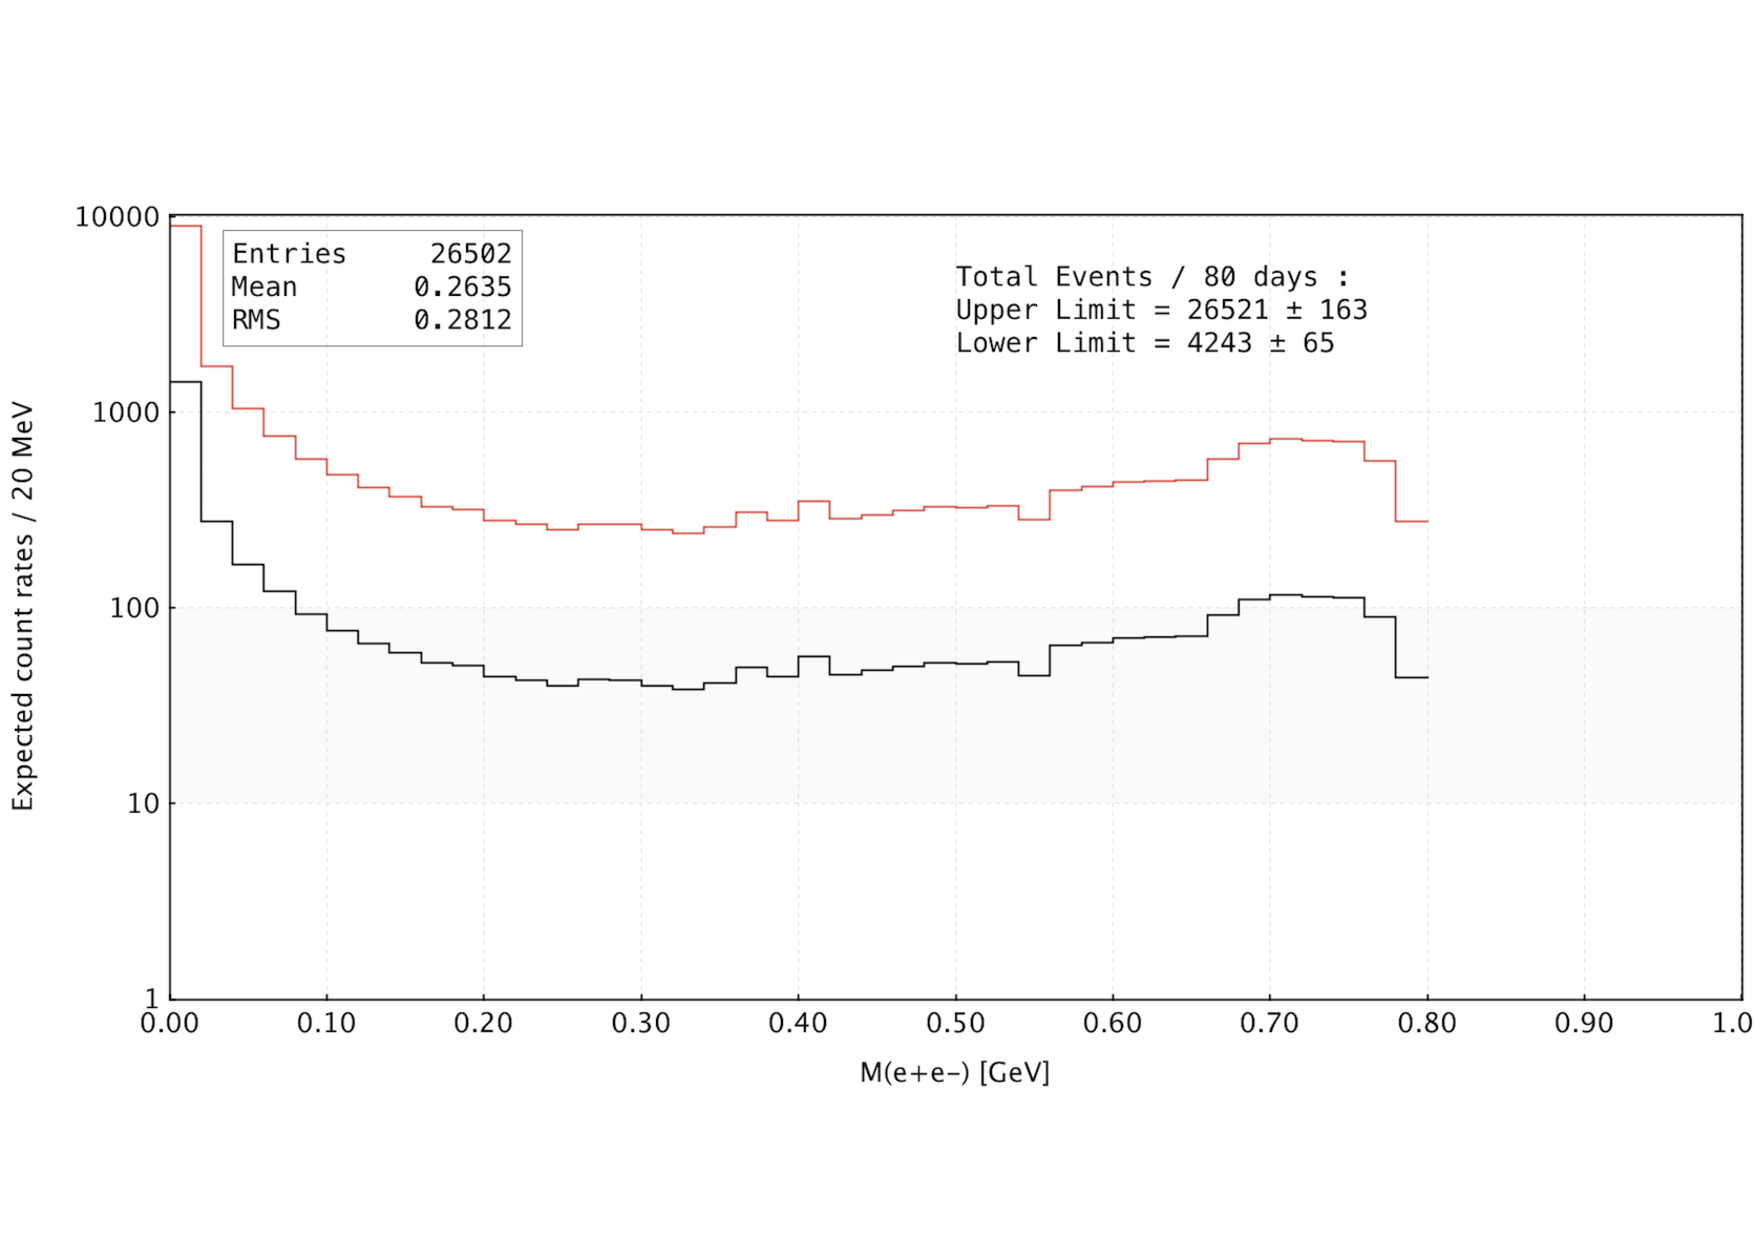
\includegraphics[width=0.8\columnwidth,height=1.0\qfigheight]{\grpath/counts/75_TORUS/VMD/VMD_Incluvise_count_rate.pdf}\label{fig:etap_count_inclu}
%	}
%\caption[Counts rates for \etaTP]{\label{fig:etayield}Count rates for the exclusive~\subref{fig:etap_count_exclu} and inclusive~\subref{fig:etap_count_inclu}. For both plots the photon detection efficiency was assumed to be between 10\%(Red) and  2\%(Black). }
%\end{center}\end{figure}
%\FloatBarrier
%Integrating over $M(\epem)$, the expected yield calculates to be $17,398$ events for exclusive scheme and $26,521$ events for the inclusive scheme. This would increase the world statistics by a factor of $\sim 20$ and $\sim 30$ respectively. 
%Table~\ref{tab:counts} and Tab.~\ref{tab:countsfull} in App.~\ref{sec:app.rates} depicts the upper and lower amount of \epemT expected from 80 days of beam time for two torus fields of 75\% and 100\% respectively.
%\FloatBarrier
%%\subsection{Realistic Yield}
%%As a reality check, lets compute the number of $\etaP \to \epem \gamma$ that g12 would have seen, had the experiment ran for 80 days with a real photon flux as calculated for CLAS12 (Sec.~\ref{sec:calflux}). %with the \epemT trigger configuration
%%The 89 $\etaP \to \epem \gamma$ events produced in g12 were recorded when the \epemT trigger was established. This time was 66\% of the total 44 days, which is $\sim29$ days. The total integrated flux measured during this time was $\sim 8.8\cdot 10^{13}$ photons. Therefore, in 80 days the total integrated flux would have been $\sim 2.4\cdot 10^{14}$ and the total number of \etaPDal \ events recorded would have been 242. The ratio of g12 total flux at 80 days per CLAS12 real photon flux is $2.73\cdot 10^{16} / 2.4\cdot 10^{14} \sim 114 $. Therefore g12 would have recorded $114\cdot 242 = 27590$ \etaPDal \ events, which is consistent with what is proposed to be measured with 80days, in the inclusive reconstruction scheme for either torus field setting. See Sec.~\ref{sec:app.rates} for total count rates.
\subsection{Acceptance at 100\% Torus field}
An addition simulation was performed using the same generated data shown above, the difference being the setting of the torus magnetic field. Below, in Fig.~\ref{fig:ratio}, the ratio of the lepton acceptance for the two different torus settings is depicted.
\begin{figure}[h!]\begin{center}
 		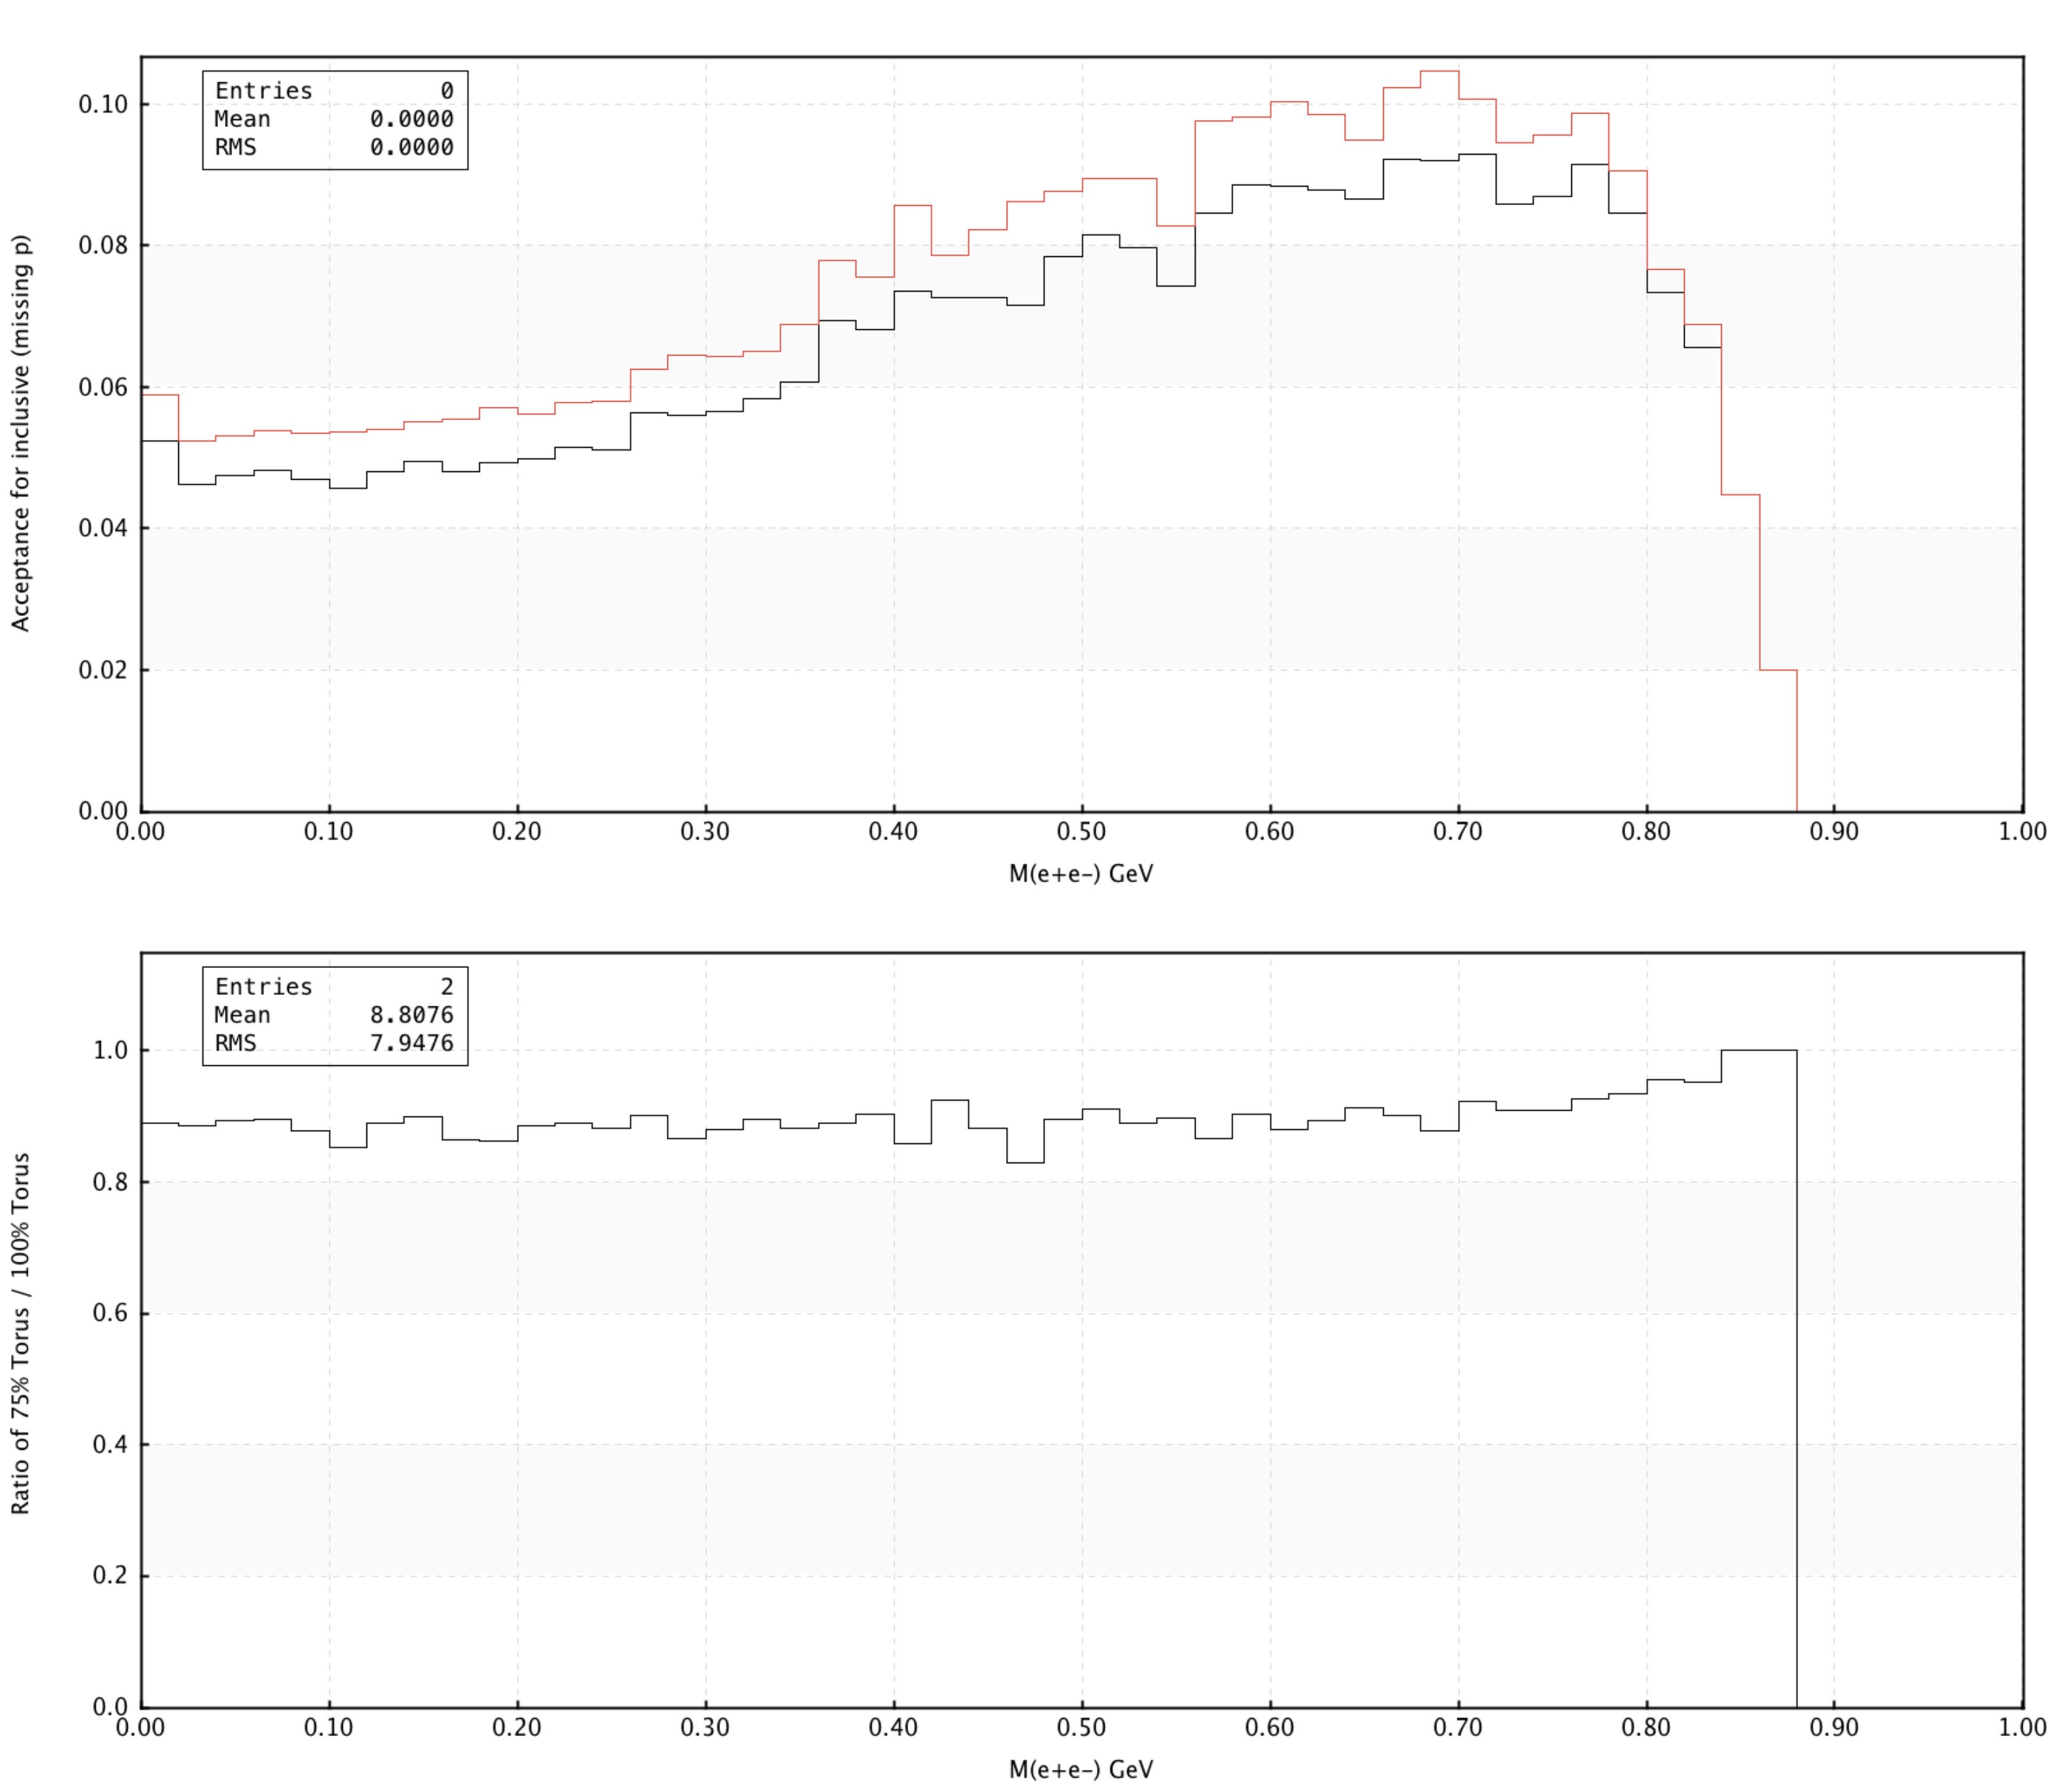
\includegraphics[width=\figwidth,height=1.6\qfigheight]{\grpath/counts/Ratio.pdf}
 		\caption[Acceptance, as a function of $M(\epem)$]{\label{fig:ratio}{Acceptance using a VMD decay model, as a function of $M(\epem)$ for the inclusive scheme(Top). The torus field was set to 75\%(red) as well as 100\%(black). Ratio of the acceptances plotted above (75\%/100\%)(Bottom). }}
\end{center}\end{figure}
\FloatBarrier
\subsection{Expected Systematic Uncertainties}
The major sources of systematic uncertainties are the acceptance and particle identification. The lepton acceptance uncertainty is estimated to be $\lesssim$ 5\% which was observed in former CLAS experiments. The lepton identification uncertainty will arise from the performance of the HTCC, PCAL and EC. From simulation studies performed for this proposal, all leptons and final state photons are detected within the geometric space of the PCAL+EC with hit coincidences in both. Furthermore, all leptons, within a few percent, that were detected in the PCAL+EC were also detected in the HTCC. Further systematics from pion contamination are mitigated by the pion rejection factor described above. Systematics related to external photon conversion are minimal due to the  1~mm resolution of the primary vertex given by the Silicon Vertex Tracker (SVT) as shown in Sec~\ref{sec:intro.conversion}. Any Bethe-Heitler contributions are negligible when utilizing and exclusive meson reconstruction scheme.




%\section{Manpower}\label{sec:manpower}
To analyze the \etaPDal \ and \phiDal \ decays, a minimum of one postdoctoral associate and one graduate student will be needed~\todo{or allotted?} to perform the following tasks:
\begin{itemize}
	\item Aide in the calibration of RunGroupA
	\item Skimming and analyzing the \epemT \ data
	\item Simulating and correcting the data
	\item Writing the publications of the results
\end{itemize}

\section{Beam Time Request}
With this proposal and beam time request, we ask for 100 days of beam time. Of the 100 days, 80 days will be dedicated to the production beam time with the standard CLAS setup, at full luminosity ($\sim 10^{35} \mathrm{cm^{-2}s^{-1}}$) with 75\% torus field. The remaining 20 days will be dedicated to optimizing and testing the trigger set-up (HTCC +PCAL + EC). This request should provide a competitive data sample of $\etaP \to \epem \gamma$ and $\phi \to \epem \eta$. The CLAS12 configuration we propose for the measurement of the transition form factors is compatible with the experimental setup already established by Run Group A.
%\section{Summary}

\newpage
\clearpage
\phantomsection 
\addcontentsline{toc}{section}{BIBLIOGRAPHY}
\bibliographystyle{unsrt}
\bibliography{Meson}	

\newpage
\addcontentsline{toc}{section}{APPENDICES}
\let\oldaddtocontents\addtocontents \renewcommand{\addtocontents}[2]{}
\begin{appendices} 
	\section{Appendix}\label{sec:app}

\subsection{$\etaP$ Decays}\label{sec:decays}
 Figure~\ref{fig:piz.alldecay} illustrates the Feynman diagrams for the ``Two photon decay'' and the ``Dalitz decay''.
%Table~\ref{tab:pi0}. Figure~\ref{fig:piz.alldecay} illustrates the Feynman diagrams for the ``Two photon decay'' and the ``Dalitz decay''.
\begin{figure}[h!]\begin{center}
\subfloat[Feynman Diagram of $\etaP$ Two Photon Decay][]{ %Feynman diagram of $\etaP$ two photon decay
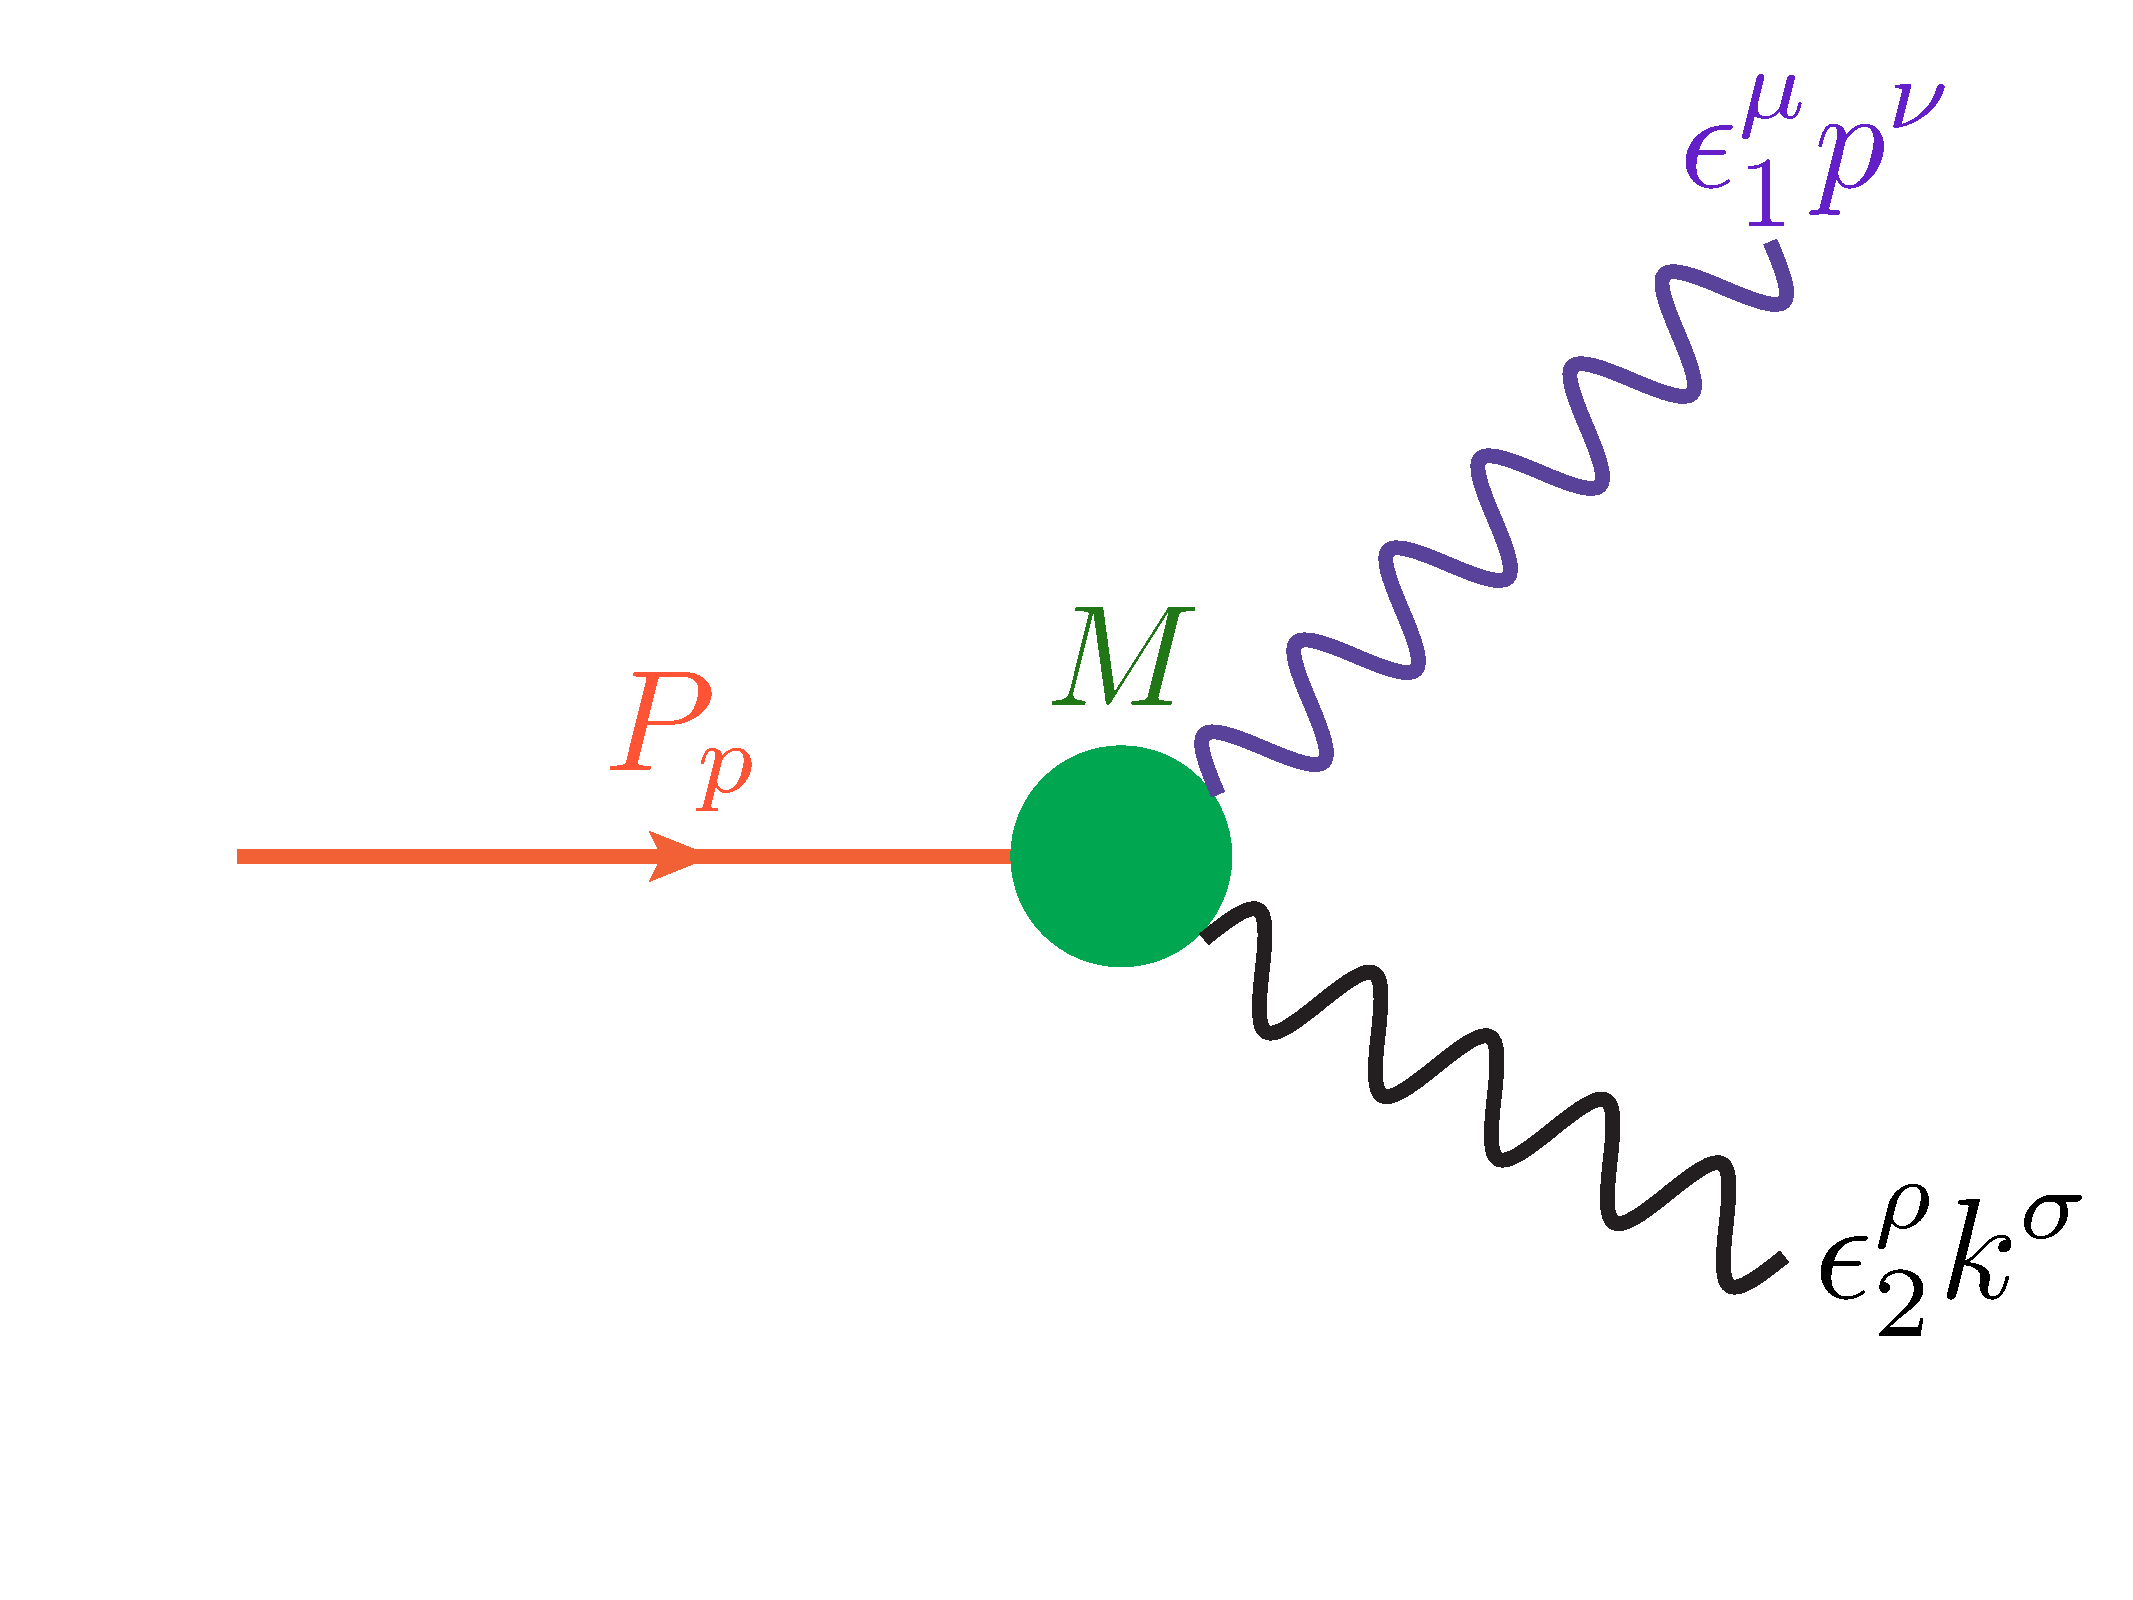
\includegraphics[width=0.65\columnwidth,height=0.65\qfigheight]{\grpath/decays/P_to_gamgam_wnotation.pdf}\label{fig:piz.gamgam}
}

\subfloat[Feynman Diagram of $\etaP$ Dalitz Decay][]{ %Feynman diagram of $\etaP$ Dalitz decay
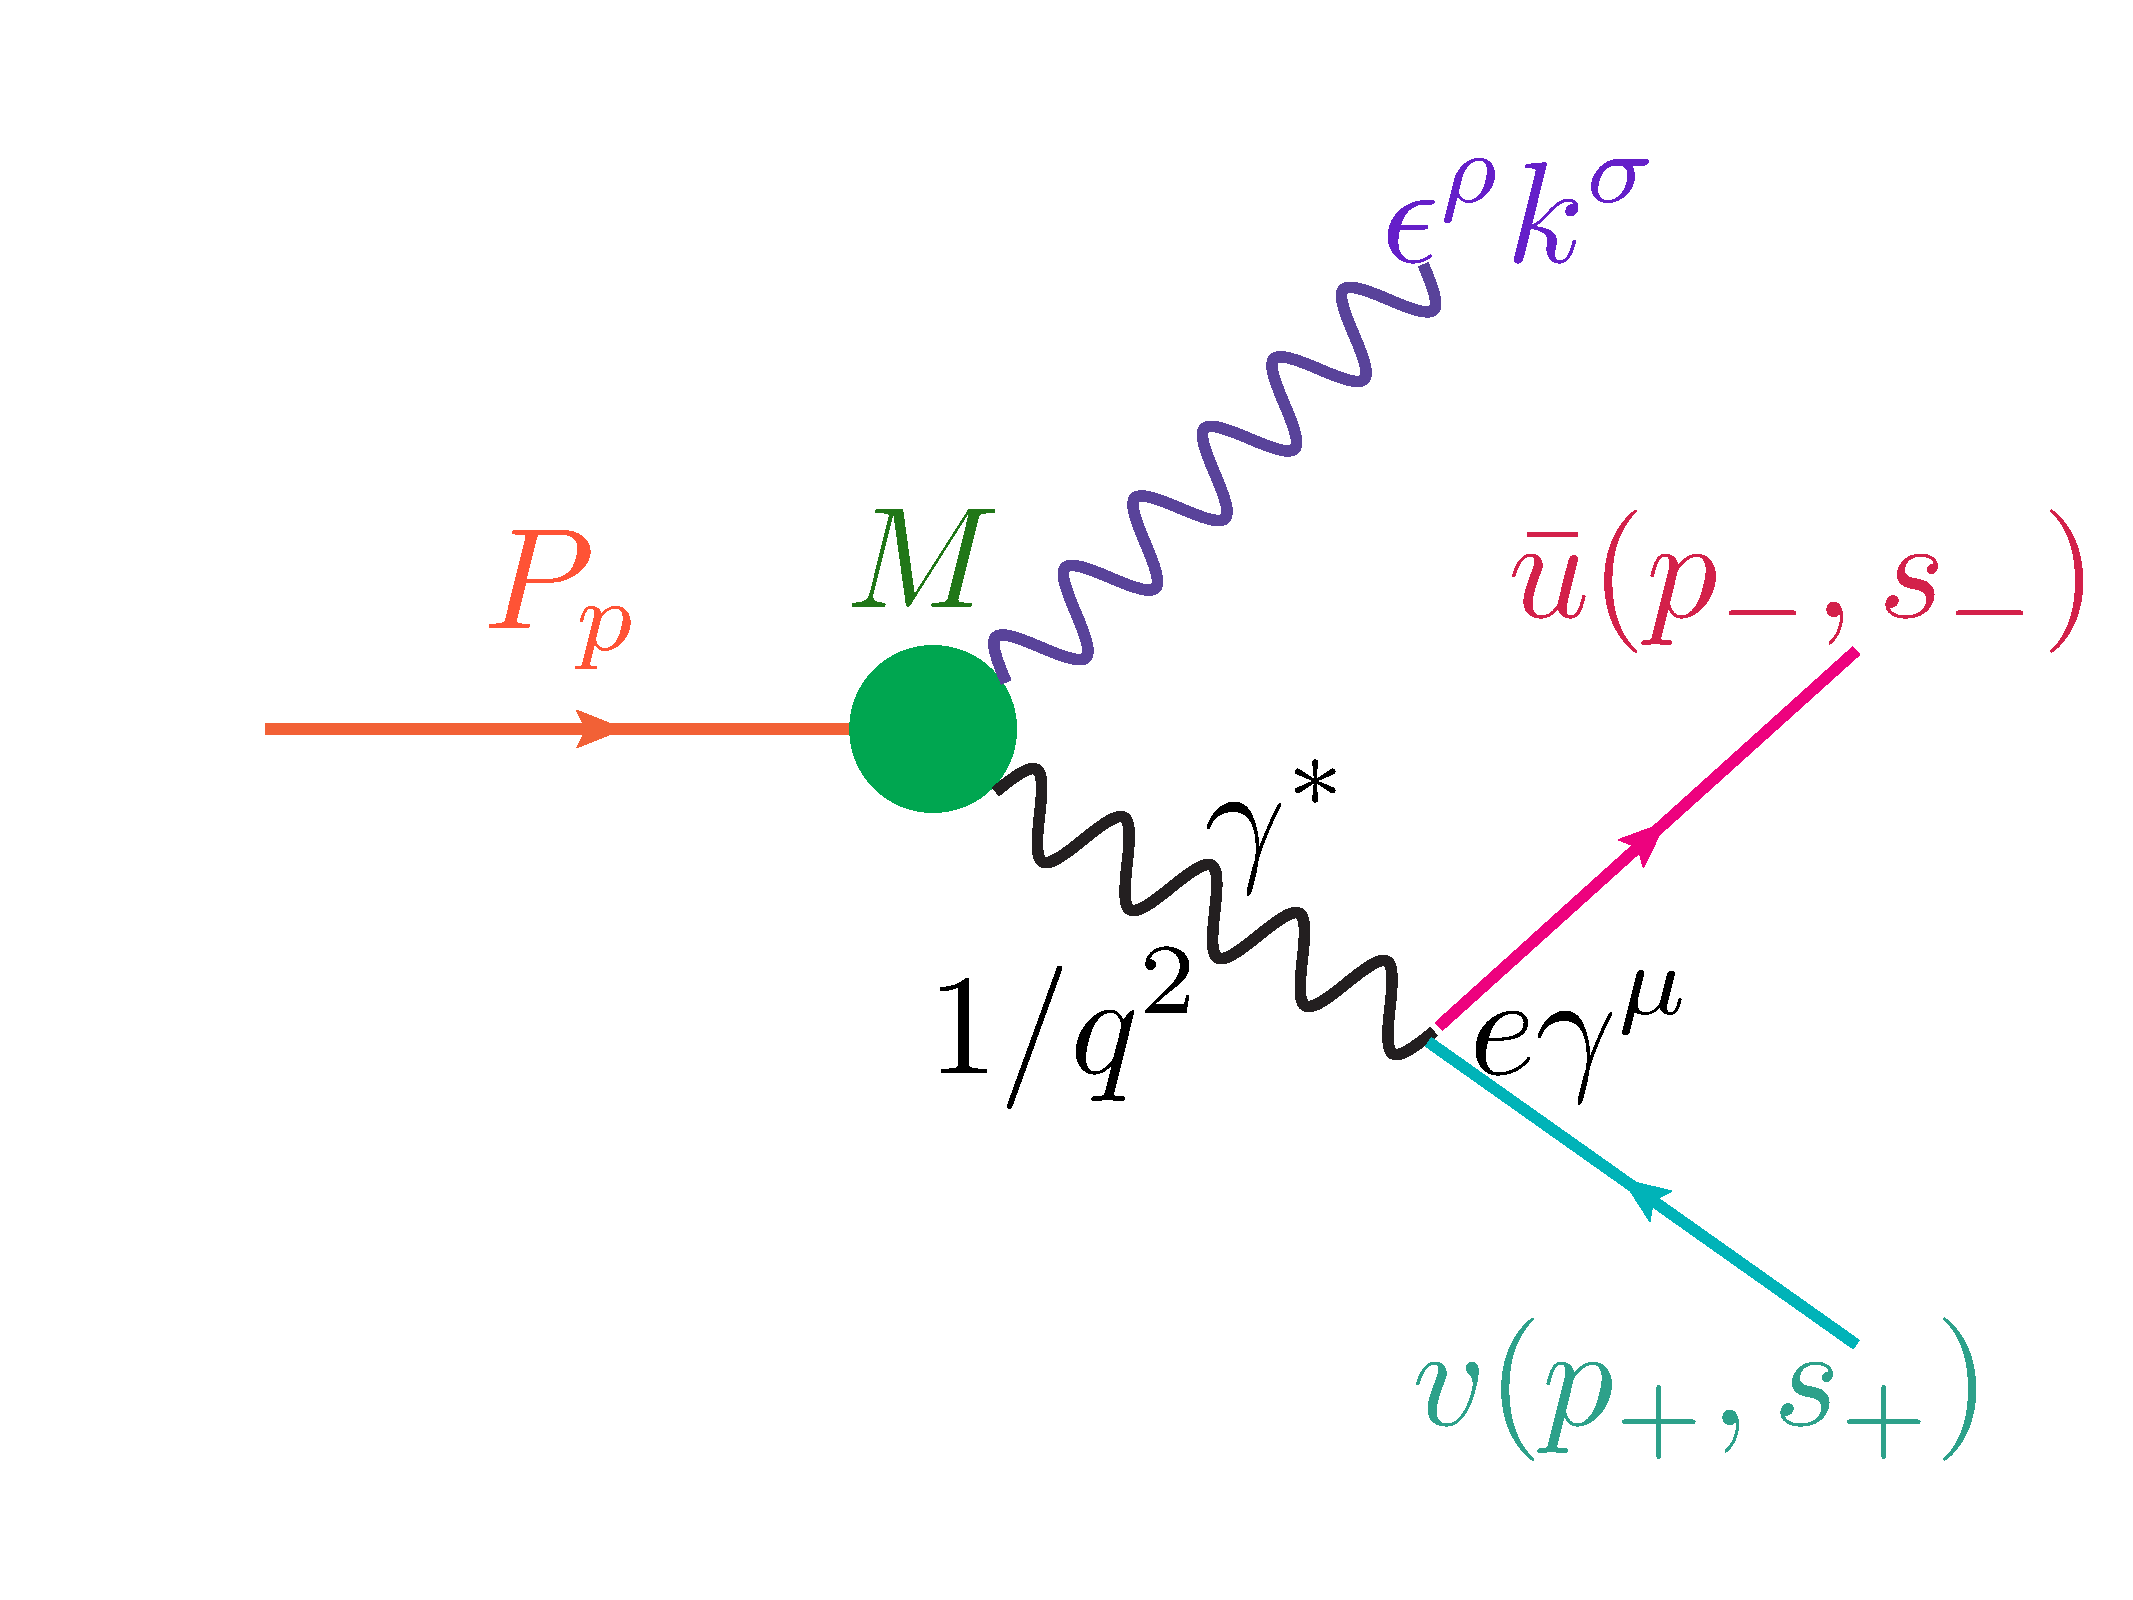
\includegraphics[width=0.65\columnwidth,height=0.65\qfigheight]{\grpath/decays/P_to_lepsgam_wnotation.pdf}\label{fig:piz.dalitz}
}
\caption[Feynman diagram of $P_p$($\etaP$) two photon decay and Dalitz decay]{\label{fig:piz.alldecay}Feynman diagram of $P_p$($\etaP$) two photon decay~\subref{fig:piz.gamgam}, $\epsilon_1$ and $\epsilon_2$ are the polarizations, $p$ and $k$ are 4-momenta of the photons.  Feynman diagram of $P_p$($\pi^0$) Dalitz decay~\subref{fig:piz.dalitz}, the variable $s_\pm$ are the spin helicities of the outgoing leptons $l^\pm$ with 4-momenta $p_{\pm}$ and $\epsilon$ is the polarization of the outgoing photon with 4-momenta $k$. In both diagrams $\mathcal{M}$ is the form factor.}

\end{center}\end{figure}
%\FloatBarrier
\subsection{Two Photon Decay}\label{sec:piz.gg}
As shown in Fig.~\ref{fig:piz.gamgam}, the two photon decay can be expressed in terms of the respective momentum, $P_p$($\eta^{\prime}$)$\to \gamma(\epsilon_1,p) \gamma(\epsilon_2,k)$, where $\epsilon_1$ and $\epsilon_2$ are the polarizations of the photons with 4-momenta $p$ and $k$. Dropping the nomenclature ($\eta^{\prime}$) in $P_p$($\eta^{\prime}$), the four momentum of the decaying meson is $P_p= p+k$. Using the Feynman rules as given in~\cite{peskin}and~\cite{halzen}, which are Lorentz and gauge invariant and also parity conserving, the amplitude can be solved to be:

\begin{align}\label{eq:piz.gg.amp}
 {\cal M}(P_P \to \gamma(\epsilon_1,p) \gamma(\epsilon_2,k))= {M}_P(p^2=0,k^2=0) \varepsilon_{\mu\nu\rho\sigma}\epsilon_1^\mu p^\nu \epsilon_2^\rho k^\sigma
\end{align}
where $\varepsilon_{\mu\nu\rho\sigma}$ is the antisymmetric metric tensor. The form factor, ${M}_P(p^2=0,k^2=0)$, contains information of the decaying meson and since the decay products are on-shell photons, which are massless, ${M}_P$ is a constant given as;
\begin{align}\label{eq:decay.constants}
 {M}_P=\begin{cases}
         {\displaystyle\frac{\alpha}{\pi f_{\pi}}} & \mbox{if $P=\etaP$};\\
        {\displaystyle\frac{\alpha}{\pi f_\pi} \frac{1}{\sqrt{3}} }\left( \frac{f_\pi}{f_8} \cos\theta_{mix} -2\sqrt{2} \frac{f_\pi}{f_0} \sin\theta_{mix} \right)& \mbox{if $P=\eta$};\\
        {\displaystyle\frac{\alpha}{\pi f_\pi} \frac{1}{\sqrt{3}}} \left( \frac{f_\pi}{f_8} \sin\theta_{mix} +2\sqrt{2} \frac{f_\pi}{f_0} \cos\theta_{mix} \right)& \mbox{if $P=\eta'$} \,
\end{cases}
\end{align}
where $\alpha=e^2/4\pi \approx 1/137$ is the fine structure constant, $f_\pi \approx 92.4 \,{\rm MeV}$ is the physical value of the pion-decay constant and $f_0 \approx 1.04 f_\pi$ and $f_8 \approx 1.3 f_\pi$ are the singlet and octet Pseudo-Goldstone meson decay constants.

\subsubsection{\emph{Squared Matrix Element}}
The squared matrix element of the decay $P_P \to \gamma(\epsilon_1,p) \gamma(\epsilon_2,k)$ is given by
\begin{align}\label{eq:piz.gg}
\left|{\cal  M}(P_{P}\rightarrow\gamma(\epsilon_{1},p)\gamma(\epsilon_{2},k))\right|^{2}=\left|M_{P}\right|^{2}\varepsilon_{\mu\nu\rho\sigma}\varepsilon_{\mu^{\prime}\nu^{\prime}\rho^{\prime}\sigma^{\prime}}\epsilon_{1}^{\mu}p^{\nu}\epsilon_{2}^{\rho}k^{\sigma}\epsilon_{1}^{\mu^{\prime}}p^{\nu^{\prime}}\epsilon_{2}^{\rho^{\prime}}k^{\sigma^{\prime}}
%
\end{align}
which can be simplified to;
\begin{align}\label{eq:piz.gg.simplify}
\left|{\cal M}(P_{P}\to\gamma(p)\gamma(k))\right|^{2}=\left|M_{P}\right|^{2}\varepsilon_{\mu\nu\rho\sigma}\varepsilon^{\mu\nu}_{\quad \rho^{\prime}\sigma^{\prime}}p^{\rho}p^{\rho^{\prime}}k^{\sigma}k^{\sigma^{\prime}}
%
\end{align}
by assuming that the polarizations of the photons remain unobserved, as they are in \abbr{CLAS}. Therefore the photon polarization vectors can be summed using Eq.~5.75 from~\cite{peskin} which reads as;
\begin{align}
\sum\limits_{polarizations} \epsilon_{\mu} \epsilon_{\mu^{\prime}} \to -g_{\mu\mu^{\prime}} 
\end{align}
As indicated in ~\cite{peskin}, the right arrow indicates that this is not an actual equality, but the solution is valid as long as both sides are dotted into Eq.~\ref{eq:piz.gg}. The antisymmetric tensor, $\varepsilon_{\mu\nu\rho\sigma}\varepsilon^{\mu\nu}_{\quad \rho^{\prime}\sigma^{\prime}}$ is simplified using  Eq.~A.30 of \cite{peskin}; 
\begin{align}\label{eg:antiT_ID}
\varepsilon_{\mu\nu\rho\sigma}\varepsilon^{\mu\nu}_{\quad \rho^{\prime}\sigma^{\prime}} = -2(g_{\rho\rho^{\prime}}g_{\sigma\sigma^{\prime}} - g_{\rho\sigma^{\prime}}g_{\rho^{\prime}\sigma})\\
\end{align}
Applying Eq.~\ref{eg:antiT_ID} to Eq.~\ref{eq:piz.gg.simplify} results in;
\begin{align}\label{eq:piz.gg.reduced}
\left|{\cal M}(P_{P}\to\gamma(p)\gamma(k))\right|^{2}=\left|M_{P}\right|^{2}(-2)(p^2k^2 - (p\cdot k)^2) \ .
%
\end{align}
Substituting
\begin{align}
(p + k)^2 = p^2 + k^2 +2 (p\cdot k) \ ,
\end{align}
and applying $p^2= k^2=0$, since both photons are massless because they are on-shell, we can derive the final expression of the squared amplitude of the decay $P_P \to \gamma(\epsilon_1,p) \gamma(\epsilon_2,k)$ as;
\begin{align}\label{eq:piz_gg_amp_final}
\left|{\cal M}(P_{P}\to\gamma(p)\gamma(k))\right|^{2}= \left|M_{P}\right|^{2}\frac{1}{2}(p+k)^{4} = \frac{1}{2}\left|M_{P}\right|^{2}m_{P}^{4}
\end{align}
where $m_P^4$ is the mass of the \etaTP derived from the 4-momenta conservation equation $(p+k)^4 = m_P^4$
\subsubsection{\emph{Decay rate}}
The decay rate of a two-body decay is explained in Equation 46.17 of~\cite{pdg2014} as
\begin{align}\label{eq:pdg.2body}
d\Gamma = \frac{1}{32 \pi^2} A \left|{\cal M}\right|^2\frac{\left|\bf{p_1}\right|}{m_p^2}d\Omega \ ,
\end{align}
where $d\Omega$ is the solid angle of particle 1 and $A$ is the symmetry factor which appears because of the Bose symmetry of the two
outgoing photons. Substituting the square matrix element from Eq.~\ref{eq:piz_gg_amp_final} into Eq.~\ref{eq:pdg.2body} and integrating over the solid angle yields;
\begin{align}
\Gamma_{P\rightarrow\gamma\gamma} = \frac{1}{32\pi^{2}} \frac{1}{2} \left|{\cal M}(P_{P}\to\gamma(p)\gamma(k))\right|^{2} \frac{\left|\bf{p}\right|}{m_{P}^2} 4 \pi = \frac{1}{32 \pi}\left|M_{P}\right|^{2}m_{P}^{2}\left|\bf{p}\right|
\end{align} 
Finally, in the center-of-mass (C.M.) frame of the decaying meson, $\bf{p} = E_{\gamma}^{C.M.} = \frac{m_p}{2}$, we find the final expression of the decay rate of $P_P \to \gamma(\epsilon_1,p) \gamma(\epsilon_2,k)$ as;
\begin{align}\label{eq:piz.gg.decay.final}
\Gamma_{P\rightarrow\gamma\gamma} = \frac{1}{64\pi} \left|M_{P}\right|^{2}m_{P}^{3} \ .
\end{align}


%
\subsubsection{\emph{Photon Conversion to \epem Pairs}}\label{sec:intro.conversion}
When a photon travels through matter at energies greater than 100~MeV, it can convert into an electron-positron pair. The process of pair production, $\gamma Z \rightarrow Ze^{+}e^{-}$, occurs when a photon with $E_0 > 2 m_e c^2$ converts into an electron and a positron. The cross section for this process can be written as;
\begin{equation}\label{pair_crosssection}
\sigma_{\gamma\rightarrow e^+e^-} =  \frac{A}{N_{A} \rho \lambda_\gamma}  \ ,\ \lambda_\gamma = \frac{9}{7}X_0
\end{equation}
where $\lambda$ is the interaction length, or mean free path, $\rho$ is the density of the material, $N_A$ is Avogadro's number and $A$ is the atomic mass of the material. The probability of pair production to occur is solely based on $X_{0}$, the radiation length of the medium and this probability can be expressed as;
\begin{equation}
\frac{dP}{dx} = \frac{1}{\lambda_\gamma}\exp(\frac{-x}{\lambda_\gamma}) \ .
\end{equation}
%
%
The probability of pair production when a photon, from the $\etaP \to \gamma \gamma$ decay, traveling though 5~cm of liquid hydrogen, $\ell$H$_2$, is shown in Fig.~\ref{fig:conversion}. 
\begin{figure}[h!]\begin{center}
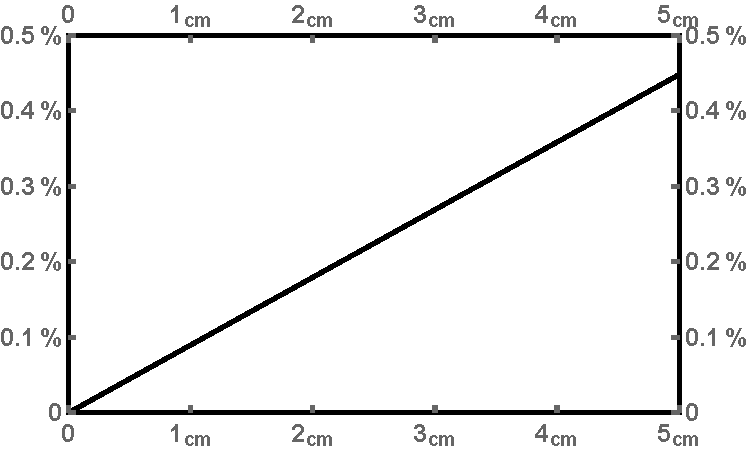
\includegraphics[width=\figwidth,height=\qfigheight]{\grpath/decays/Hydrogen_conversion_Prob_CLAS12.pdf}
\caption[Probability of pair production, $\gamma \to$\epem, as a function of distance in liquid hydrogen]{\label{fig:conversion}{Probability of pair production, $\gamma \to$\epem, as a function of distance in liquid hydrogen.}}
\end{center}\end{figure}
Since CLAS12 has a vertex resolution of $\approx$1~mm the probability of pair production traveling through 10~mm is shown in Fig.~\ref{fig:conversionmm}. 
\begin{figure}[h!]\begin{center}
		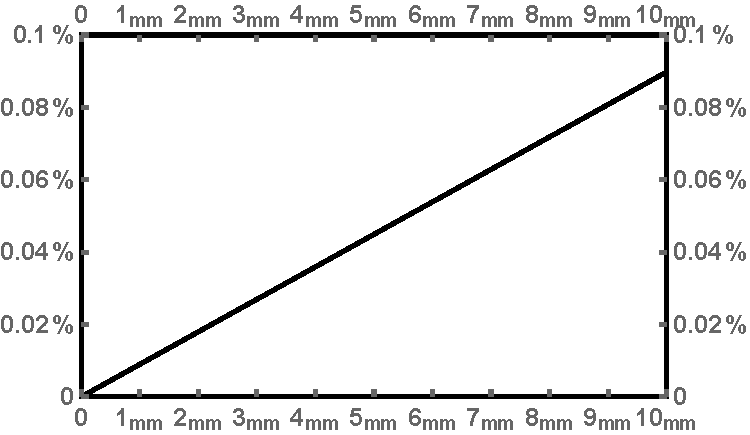
\includegraphics[width=\figwidth,height=\qfigheight]{\grpath/decays/Hydrogen_conversion_Prob_CLAS12mm.pdf}
		\caption[Probability of pair production, $\gamma \to$\epem, as a function of distance in liquid hydrogen]{\label{fig:conversionmm}{Probability of pair production, $\gamma \to$\epem, as a function of distance in liquid hydrogen.}}
	\end{center}\end{figure}
This type of subprocess mimics the Dalitz decay  $\etaP \to e^+e^- \gamma$, described in Sec.~\ref{sec:dalitzdecay}. Since there are 2 photons with equal probability of conversion, the total probability is double that shown in Fig.~\ref{fig:conversion}.



%\subsection{$\etaP$ Dalitz Decay}\label{sec:dalitzdecay} 
When a pseudoscalar meson decays via a photon $\gamma$ and a dilepton ($l^{+}l^{-}$) pair, it is known as a Dalitz decay or a so-called single off-shell decay. The Dalitz decay is related to the two photon decay. However, in the Dalitz decay, one of the photons is off-shell ($\gamma^*$) and decays into a dilepton pair. Since the Dalitz decay is related to the two photon decay, the form factor of the Dalitz decay, for P($\eta'$), will be similar to the form factor of the two photon decay of P( $\eta'$), except there will be an effective mass dependence for the Dalitz decay. Figure~\ref{fig:piz.dalitz} depicts the Feymann diagram of the Dalitz decay.

The amplitude for the decay $P_P \to \gamma^\star(p) \gamma(k) \to l^+(p_+)l^-(p_-) \gamma(k)$ is given by the following expression:
\begin{align}\label{eq:piz.eeg.amp}
{\cal M}(P\to l^+(p_+,s_+)l^-(p_-,s_-) \gamma) = &{M}_P(p^2,k^2=0) \varepsilon_{\mu\nu\rho\sigma} \frac{1}{q^2} \nonumber \times \left[\right. \\ 
&\left. e \bar u(p_-,s_-) \gamma^\mu v(p_+,s_-) q^\nu \epsilon^\rho k^\sigma \right] .
\end{align}
Comparing the amplitudes of Eq.~\ref{eq:piz.eeg.amp} and Eq.~\ref{eq:piz.gg.amp} it is seen that the polarization of the off-shell photon turned into the current $e \bar u(p_-,s_-) \gamma^\mu v(p_+,s_-)$ of the lepton pair. The parameters $s_\pm$ are the spin helicities of the outgoing leptons $l^\pm$ and as in  Eq.~\ref{eq:piz.gg}, $\epsilon$ is the polarization of the outgoing photon. 
%
\subsubsection{\emph{Squared Matrix Element}}


\begin{align}\label{eq:piz.eeg}
&\left|{\cal M}(P\to l^+(p_+,s_+)l^-(p_-,s_-) \gamma)\right|^2 =  \frac{e^2}{q^4} \left|M\right|^2  \varepsilon_{\mu\nu\rho\sigma}\varepsilon_{\mu^{\prime}\nu^{\prime}\rho^{\prime}\sigma^{\prime}}   \nonumber \times \left[\right.
\\ & \left.\bar u(p_-,s_-) \gamma^\mu v(p_+,s_+) \bar v(p_+,s_+) \gamma^{\mu^{\prime}}  u(p_-,s_-) q^\nu \epsilon^\rho k^\sigma q^{\nu^{\prime}} \epsilon^{\rho^{\prime}} k^{\sigma^{\prime}}\right] .
%
\end{align}
using an equation found between equation 5.3 and 5.4 found in~\cite{peskin}
\begin{align}\label{eq:spin.sum}
& \sum\limits_{s_{-},s_{+}}^{} \bar{u}(p_{-},s_{-})\gamma^{\mu}\nu(p_{+},s_{+})\bar{\nu}(p_{+},s_{+})\gamma^{\mu^{\prime}}u(p_{-},s_{-}) = Tr\left[ (\slashed{p}_- +m)\gamma^{\mu} (\slashed{p}_+-m)\gamma^{\mu^{\prime}} \right]\nonumber \\ & =2q^{2}\left[-(g_{\mu\mu^{\prime}}-\frac{p_{\mu}p_{\mu^{\prime}}}{q^{2}} ) - \frac{(p_{+} - p_{-})_{\mu}(p_{+} - p_{-})_{\mu^{\prime}}}{q^{2}}\right]
\end{align}
where the identity $q = p_+ + p_-$ was used.
Substituting Eq.~\ref{eq:spin.sum} into Eq.~\ref{eq:piz.eeg}
\begin{align} \label{eq:piz.eeg.midway1}
\left|{\cal M}\right|^{2} = &  \frac{2e^{2}\left|M_{P}\right|^{2}}{q^{2}}\varepsilon_{\mu\nu\rho\sigma}\varepsilon_{\mu^{\prime}\nu^{\prime}\rho^{\prime}\sigma^{\prime}}\left[-g^{\mu\mu^{\prime}} - \frac{(p_{+} - p_{-})^{\mu}(p_{+} - p_{-})^{\mu^{\prime}}}{q^{2}}\right]
\times \nonumber \\ &\left[ (-g^{\nu\nu^{\prime}})q^{\rho}k^{\sigma}q^{\rho^{\prime}}k^{\sigma^{\prime}} \right]
\end{align}
Substituting $k = P - q$ and $p_- = q - p_+$ into Eq.~\ref{eq:piz.eeg.midway1}
\begin{align} \label{eq:piz.eeg.midway2}
\left|{\cal M}\right|^{2} = & \frac{2e^{2}\left|M_{P}\right|^{2}}{q^{2}}\varepsilon_{\mu\nu\rho\sigma}\varepsilon_{\mu^{\prime}\nu^{\prime}\rho^{\prime}\sigma^{\prime}}\left[-g^{\mu\mu^{\prime}} - \frac{(2p_{+} - q)^{\mu}(2p_{+} - q)^{\mu^{\prime}}}{q^{2}}\right] \times \nonumber \\ &  (-g^{\nu\nu^{\prime}})      
(q^{\rho}P^{\sigma} - q^{\rho}q^{\sigma}) (q^{\rho}P^{\sigma^{\prime}} - q^{\rho^{\prime}}q^{\sigma^{\prime}})
\end{align}
Applying properties of $-g^{\mu\mu^{\prime}}$ and $-g^{\nu\nu^{\prime}}$ onto Eq.~\ref{eq:piz.eeg.midway2}
\begin{align} \label{eq:piz.eeg.midway3}
\left|{\cal M}\right|^{2} = \frac{2e^{2}\left|M_{P}\right|^{2}}{q^{2}}
& \left[\varepsilon_{\mu\nu\rho\sigma}\varepsilon^{\mu\nu}_{\quad \rho^{\prime}\sigma^{\prime}}q^{\rho}P^{\sigma}q^{\rho^{\prime}}P^{\sigma^{\prime}} +
\right. \nonumber \\ & \left. \frac{4}{q^2} \varepsilon_{\mu\nu\rho\sigma}\varepsilon^{\mu}_{\ \ \nu^{\prime} \rho^{\prime}\sigma^{\prime}} p_{+}^{\nu}p_{+}^{\nu^{\prime}}q^{\rho}q^{\rho^{\prime}}P^{\sigma}P^{\sigma^{\prime}}\right]
\end{align}
Switching to the rest frame of the pseudoscalar meson, $P_p$, the 4-momenta is transformed to $P^\sigma = m_p\delta^{\sigma 0}$. The squared amplitude of Eq.~\ref{eq:piz.eeg.midway3} reads;
\begin{align} \label{eq:piz.eeg.midway4}
\left|{\cal M}\right|^{2} = & \frac{2e^{2}\left|M_{P}\right|^{2}}{q^{2}}m_p^2
\left[\varepsilon_{\mu\nu\rho}\varepsilon^{\mu\nu}_{\ \ \rho^{\prime}}q^{\rho}q^{\rho^{\prime}} - \frac{4}{q^2} \varepsilon_{\mu\nu\rho}\varepsilon^{\mu}_{\ \nu^{\prime}\rho^{\prime}} p_{+}^{\nu}p_{+}^{\nu^{\prime}}q^{\rho}q^{\rho^{\prime}}\right]
\end{align}
The sign change is due to $g^{\sigma \sigma^{\prime}} = -\delta^{\sigma \sigma^{\prime}}$. 
Using the antisymmetric tensor properties $\varepsilon_{\mu\nu\rho}\varepsilon^{\mu\nu}_{\ \ \rho^{\prime}} = 2\delta_{\rho\rho^{\prime}}$ and $\varepsilon_{\mu\nu\rho}\varepsilon^{\mu}_{\ \nu^{\prime}\rho^{\prime}} = \delta_{\nu\nu^{\prime}}\delta_{\rho\rho^{\prime}} - \delta_{\nu\rho^{\prime}}\delta_{\rho\nu^{\prime}} = (\hat{e}_{\nu} \times \hat{e}_{\rho}) \cdot (\hat{e}_{\nu^{\prime}} \times \hat{e}_{\rho^{\prime}})$, Eq.~\ref{eq:piz.eeg.midway4} is reduced to 
\begin{align} \label{eq:piz.eeg.final}
\left|{\cal M}\right|^{2} =  \frac{2e^{2}\left|M_{P}\right|^{2}}{q^{2}}m_p^2
\left[2\left|\bf{q}\right|^2 - \frac{4}{q^2} \left|\bf{q}\right|^2 \left|\bf{p_{+}}\right|^2 \sin^2(\theta_{p_{_+}q}) \right]
\end{align}

\subsubsection{\emph{Decay rate}}
The decay rate of a three-body decay is given in Equation 46.19 of~\cite{pdg2014} as
\begin{align}\label{eq:pdg.3body}
d\Gamma = \frac{1}{(2 \pi)^5} \frac{1}{16 m_p^2} \left|{\cal M}\right|^2 \left|\bf{p_1^*}\right| \left|\bf{p_3}\right|d\Omega_1^*d\Omega_3 dm_{12} \ ,
\end{align}
%
where ($\left|\bf{p_1^*}\right|,\Omega_1^*$) is the momentum of particle 1 in the rest frame of 1 and 2, and $\Omega_3$ is the angle of particle 3 in the rest frame of the decaying particle $m_p$~\cite{pdg2014}. Relating Eq.~\ref{eq:pdg.3body} to the variables in Eq.~\ref{eq:piz.eeg.final}, where $(\left|\bf{p_1^*}\right|,\Omega_1^*) = (\left|\bf{p_+}\right|,\Omega_{p_{_+}q})$, $m_{12} = q$ and $(\left|\bf{p_3}\right|,\Omega_3) = (\left|\bf{p_k}\right|,\Omega_k)$, reads;
\begin{align}\label{eq:pdg.3body.sub}
d\Gamma = \frac{1}{(2 \pi)^5} \frac{1}{16 m_p^2} \left|{\cal M}\right|^2 \left|\bf{p_+}\right| \left|\bf{p_k}\right|d\Omega_+d\Omega_k dq \ ,
\end{align}
%
In the rest from of the decaying particle $m_p$, the 3-momenta $\left|\bf{p_k}\right| = \left|\bf{q}\right|$ and the solid angle $\Omega_k = \Omega_q$. Substituting the square matrix element from Eq.~\ref{eq:piz.eeg.final} into Eq.~\ref{eq:pdg.3body.sub} yields;
%
\begin{align}\label{eq:pdg.3body.sub2}
d\Gamma = & \frac{1}{(2 \pi)^5} \frac{1}{16 m_p^2} \frac{2e^{2}\left|M_{P}\right|^{2}}{q^{2}}m_p^2
\left[2\left|\bf{q}\right|^2 - \frac{4}{q^2} \left|\bf{q}\right|^2 \left|\bf{p_{+}}\right|^2 \sin^2(\theta_{p_{_+}q}) \right]
 \times \left[ \nonumber \right. \\ &\left. \left|\bf{p_+}\right| \left|\bf{q}\right|d\Omega_{p_{_+}q}d\Omega_q dq\ \right].
\end{align}
The variables $\left|\bf{q}\right|$ and $\left|\bf{p_+}\right|$ can be redefined, by means of Eq.~46.20b and Eq.~46.20a of~\cite{pdg2014}, as 
\begin{align}
\left|\bf{q}\right| = \frac{m_p^2 - q^2}{2m_p} \label{eq:eeg.qeq} \\
\left|\bf{p_+}\right| = \frac{\sqrt{q^2 - 4m_l^2}}{2} = \frac{q\sqrt{1 - \frac{4m_l^2}{q^2} } } {2} =\frac{q {\cal K}  } {2}  \label{eq:eeg.p+eq} \ ,
\end{align} 
where ${\cal K} = \sqrt{1 - \frac{4m_l^2}{q^2}}$. Replacing the variables calculated in Eq.~\ref{eq:eeg.qeq} and Eq.~\ref{eq:eeg.p+eq} into Eq.~\ref{eq:pdg.3body.sub2} and collecting terms yields;
\begin{align}\label{eq:pdg.3body.sub3}
d\Gamma = \frac{1}{(2 \pi)^5} \frac{1}{16 m_p^2} \left|M_{P}\right|^{2} & \left[ \frac{2e^2 m_p^2}{8} \left( \frac{m_p^2 - q^2}{2 m_p}\right)^3\right] \times \nonumber \left[ \right. \\ &  \left.
\left( 2 -{\cal K}^2\sin^2(\theta_{p_{_+}q})\right)\frac{{\cal K}}{4 q^2}dq^2d\Omega_{p_{_+}q}d\Omega_q \right] \ ,
\end{align}
where the identity $qdq = \frac{dq^2}{2}$. Performing the integration of $\Omega_{p_{_+}q}d\Omega_q$ and replacing $e^2 = 4\pi\alpha$ transforms Eq.~\ref{eq:pdg.3body.sub3} into;
\begin{align}\label{eq:pdg.3body.sub4}
d\Gamma = \frac{1}{(2 \pi)^3} \frac{1}{32} \frac{4 \pi \alpha}{3} \left|M_{P}\right|^{2} \left[ \frac{m_p^6 \left( 1- \frac{q^2}{m_p^2}\right)^3}{m_p^3} \right]\left( 3 -{\cal K}^2\right)\frac{{\cal K}}{q^2}dq^2\ ,
\end{align}
which can be simplified further to;
\begin{align}\label{eq:eeg.final}
d\Gamma = \left(\frac{1}{64\pi} \left|M_{P}\right|^{2}m_{P}^{3} \right) \frac{2 \alpha}{3 \pi} \frac{1}{q^2} \left( 1- \frac{q^2}{m_p^2}\right)^3 \left( 1+ \frac{2m_l^2}{q^2}\right) \left( 1- \frac{4m_l^2}{q^2}\right)^{\frac{1}{2}} dq^2\ .
\end{align}
It can be seen that the first set of variables in parenthesis in Eq.~\ref{eq:eeg.final} is Eq.~\ref{eq:piz.gg.decay.final}, therefore;
\begin{align}\label{eq:eegff.finalkroll}
\frac{d\Gamma}{\Gamma_{\gamma\gamma} dq^2} = \frac{2 \alpha}{3 \pi} \frac{1}{q^2} \left( 1- \frac{q^2}{m_p^2}\right)^3 \left( 1+ \frac{2m_l^2}{q^2}\right) \left( 1- \frac{4m_l^2}{q^2}\right)^{\frac{1}{2}} 
\end{align}
which is the Kroll-Wada equation founded in~\cite{KrollWada}.
%\subsection{$\phi$ Dalitz Decay}\label{sec:phidalitzdecay} 
%%When the $\phi$ meson decays via a $\eta$ and a dilepton ($l^{+}l^{-}$) pair, it is also known as a Dalitz decay or a so-called single off-shell decay. This Dalitz decay is related to the $\eta \gamma$ decay. However, in the Dalitz decay, one of the photons is off-shell ($\gamma^*$) and decays into a dilepton pair. Since the Dalitz decay is related to the two photon decay, the form factor of the Dalitz decay, for V($\phi$), will be similar to the form factor of the $\eta \gamma$ decay of P($\phi$), except there will be an effective mass dependence for the Dalitz decay. 
%The amplitude for the decay $V_P \to \gamma^\star(p_1) \eta(p_2) \to l^+(p_+)l^-(p_-) \eta(p_2)$ is similar Eq.~\ref{eq:piz.eeg.amp}, but replacing the on-shell photon with an $\eta$:
%\begin{equation}\label{eq:phi.eeg.amp}
%{\cal M}(P\to l^+(p_+,s_+)l^-(p_-,s_-) \eta(p_2)) = {M}_P(p_{1}^2,p_{2}^2) \varepsilon_{\mu\nu\rho\sigma} \frac{1}{q^2} e \bar u(p_-,s_-) \gamma^\mu v(p_+,s_-) q^\nu \epsilon^\rho p_{2}^\sigma.
%\end{equation}
%\subsubsection{\emph{Decay rate}}
%The decay rate for the $\phi$ transition to $\eta \gamma^\star$ is derived as~\cite{landsberg}:
%\begin{align}
%\frac{d\Gamma}{\Gamma_{\eta\gamma} dq^2} = \frac{\alpha}{3 \pi} \frac{1}{q^2} \left( \left(1+ \frac{q^2}{m_{\phi}^2 - m_{\eta}^2} \right)^2 - \frac{4 m_{\phi}^2 q^2}{m_{\phi}^2 - m_{\eta}^2}\right)^\frac{3}{2} \left( 1+ \frac{2m_l^2}{q^2}\right) \left( 1- \frac{4m_l^2}{q^2}\right)^{\frac{1}{2}} \ ,
%\end{align}
% 
\end{appendices}



\end{document}